%%%%%%%%%%%%%%%%%%%%%%%%%%%%%%%%%%%%%%%%%
% Masters/Doctoral Thesis 
% LaTeX Template
% Version 2.5 (27/8/17)
%
% This template was downloaded from:
% http://www.LaTeXTemplates.com
%
% Version 2.x major modifications by:
% Vel (vel@latextemplates.com)
%
% This template is based on a template by:
% Steve Gunn (http://users.ecs.soton.ac.uk/srg/softwaretools/document/templates/)
% Sunil Patel (http://www.sunilpatel.co.uk/thesis-template/)
%
% Template license:
% CC BY-NC-SA 3.0 (http://creativecommons.org/licenses/by-nc-sa/3.0/)
%
%%%%%%%%%%%%%%%%%%%%%%%%%%%%%%%%%%%%%%%%%

%----------------------------------------------------------------------------------------
%	PACKAGES AND OTHER DOCUMENT CONFIGURATIONS
%----------------------------------------------------------------------------------------

\documentclass[
12pt, % The default document font size, options: 10pt, 11pt, 12pt
%oneside, % Two side (alternating margins) for binding by default, uncomment to switch to one side
english,%english, % ngerman for German
singlespacing, % Single line spacing, alternatives: onehalfspacing or doublespacing
%draft, % Uncomment to enable draft mode (no pictures, no links, overfull hboxes indicated)
%nolistspacing, % If the document is onehalfspacing or doublespacing, uncomment this to set spacing in lists to single
%liststotoc, % Uncomment to add the list of figures/tables/etc to the table of contents
%toctotoc, % Uncomment to add the main table of contents to the table of contents
%parskip, % Uncomment to add space between paragraphs
%nohyperref, % Uncomment to not load the hyperref package
headsepline, % Uncomment to get a line under the header
%chapterinoneline, % Uncomment to place the chapter title next to the number on one line
%consistentlayout, % Uncomment to change the layout of the declaration, abstract and acknowledgements pages to match the default layout
]{MastersDoctoralThesis} % The class file specifying the document structure

\usepackage[utf8]{inputenc} % Required for inputting international characters
\usepackage[T1]{fontenc} % Output font encoding for international characters
\usepackage{mathpazo} % Use the Palatino font by default
\usepackage{float}
\usepackage{listings}
\lstset{
  basicstyle=\ttfamily\small,
  keywordstyle=\bfseries,
  breaklines=true,            
  frame=none,               
  numbers=none,
  commentstyle=\color{green}
}

\usepackage[backend=bibtex,style=numeric,natbib=true]{biblatex} % Use the bibtex backend with the authoryear citation style (which resembles APA)

\addbibresource{main.bib} % The filename of the bibliography

\usepackage[autostyle=true]{csquotes} % Required to generate language-dependent quotes in the bibliography
\setcounter{tocdepth}{3}
\setcounter{secnumdepth}{1}

%----------------------------------------------------------------------------------------
%	MARGIN SETTINGS
%----------------------------------------------------------------------------------------

\geometry{
	paper=a4paper, % Change to letterpaper for US letter
	inner=2.5cm, % Inner margin
	outer=3.8cm, % Outer margin
	bindingoffset=.5cm, % Binding offset
	top=1.5cm, % Top margin
	bottom=1.5cm, % Bottom margin
	%showframe, % Uncomment to show how the type block is set on the page
}

%----------------------------------------------------------------------------------------
%	THESIS INFORMATION
%----------------------------------------------------------------------------------------

\thesistitle{Analysis and development of a prompt engineering ontology} % Your thesis title, this is used in the title and abstract, print it elsewhere with \ttitle
\supervisor{Prof. Claudia d'Amato} % Your supervisor's name, this is used in the title page, print it elsewhere with \supname
\examiner{} % Your examiner's name, this is not currently used anywhere in the template, print it elsewhere with \examname
\degree{Doctor of Philosophy} % Your degree name, this is used in the title page and abstract, print it elsewhere with \degreename
\author{Simone Gramegna} % Your name, this is used in the title page and abstract, print it elsewhere with \authorname
\addresses{} % Your address, this is not currently used anywhere in the template, print it elsewhere with \addressname

\subject{Biological Sciences} % Your subject area, this is not currently used anywhere in the template, print it elsewhere with \subjectname
\keywords{} % Keywords for your thesis, this is not currently used anywhere in the template, print it elsewhere with \keywordnames
\university{{UNIVERSITÀ DEGLI STUDI DI BARI \\“ALDO MORO”}} % Your university's name and URL, this is used in the title page and abstract, print it elsewhere with \univname\\

\department{{Academic Year 2023/2024}} % Your department's name and URL, this is used in the title page and abstract, print it elsewhere with \deptname
\group{{MACHINE LEARNING}} % Your research group's name and URL, this is used in the title page, print it elsewhere with \groupname
\faculty{\href{http://faculty.university.com}{Faculty Name}} % Your faculty's name and URL, this is used in the title page and abstract, print it elsewhere with \facname

\AtBeginDocument{
\hypersetup{pdftitle=\ttitle} % Set the PDF's title to your title
\hypersetup{pdfauthor=\authorname} % Set the PDF's author to your name
\hypersetup{pdfkeywords=\keywordnames} % Set the PDF's keywords to your keywords
}

\begin{document}

\frontmatter % Use roman page numbering style (i, ii, iii, iv...) for the pre-content pages

\pagestyle{plain} % Default to the plain heading style until the thesis style is called for the body content

%----------------------------------------------------------------------------------------
%	TITLE PAGE
%----------------------------------------------------------------------------------------

\begin{titlepage}
\begin{center}
{\scshape\LARGE \univname\par}\vspace{0.5cm} % University name
\textsc{\Large     \begin{figure}[H]
    \centering
    
\includegraphics[width=.6\textwidth]{Figures/logo_UNIBA_CMYK.jpg}
    \label{logo}
    \end{figure}}%\\[0.5cm] % Thesis type

\HRule \\[0.4cm] % Horizontal line
{\huge \bfseries \ttitle\par}\vspace{0.4cm} % Thesis title
\HRule \\[1.5cm] % Horizontal line
 

 
%\vfill
\large DEPARTMENT OF COMPUTER SCIENCE\\[0.3cm]
\large Master degree in Computer Science\\[0.3cm] % University requirement text
\vfill
Thesis in\\[0.4cm]

\groupname\\[2cm] 
\begin{minipage}[t]{0.4\textwidth}
\begin{flushleft} \large
\emph{Advisor:\\[0.1cm] Prof. Claudia d'Amato} \\[0.5cm]
\emph{Co-advisor:\\[0.1cm] Dott. Roberto Barile} \\[0.1cm]
\emph{Dott. Andrea Nuzzolese} \\[0.3cm]
\end{flushleft}
\end{minipage}
\begin{minipage}[t]{0.4\textwidth}
\begin{flushright} \large
\emph{Graduating:
\\[0.1cm]
Simone Gramegna}\\
\end{flushright}
\end{minipage}\\[1cm]
\HRule \\[0.4cm]\deptname\\[2cm] % Research group name and department name
%\vfill

%{\large \today}\\[4cm] % Date
%\includegraphics{Logo} % University/department logo - uncomment to place it
 
%\vfill
\end{center}
\end{titlepage}

%----------------------------------------------------------------------------------------
%	DECLARATION PAGE
%----------------------------------------------------------------------------------------

%\begin{declaration}
%\addchaptertocentry{\authorshipname} % Add the declaration to the table of contents
%\noindent I, \authorname, declare that this thesis titled, \enquote{\ttitle} and the work presented in it are my own. I confirm that:

%\begin{itemize} 
%\item This work was done wholly or mainly while in candidature for a research degree at this University.
%\item Where any part of this thesis has previously been submitted for a degree or any other qualification at this University or any other institution, this has been clearly stated.
%\item Where I have consulted the published work of others, this is always clearly attributed.
%\item Where I have quoted from the work of others, the source is always given. With the exception of such quotations, this thesis is entirely my own work.
%\item I have acknowledged all main sources of help.
%\item Where the thesis is based on work done by myself jointly with others, I have made clear exactly what was done by others and what I have contributed myself.\\
%\end{itemize}
 
%\noindent Signed:\\
%\rule[0.5em]{25em}{0.5pt} % This prints a line for the signature
 
%\noindent Date:\\
%\rule[0.5em]{25em}{0.5pt} % This prints a line to write the date
%\end{declaration}

%\cleardoublepage


%----------------------------------------------------------------------------------------
%	ABSTRACT PAGE
%----------------------------------------------------------------------------------------

\begin{abstract}
\addchaptertocentry{\abstractname} % Add the abstract to the table of contents
This thesis explores the development of a prompt engineering ontology to improve the understanding, organization, and application of large language models (LLMs) across various domains. By providing a structured representation of prompting techniques and their relationships with LLMs, the ontology serves as a valuable resource for guiding users in effectively interacting with these advanced systems.
Large Language Models (LLMs) are AI models based on large neural networks, trained on vast amounts of text to understand and generate natural language. Those models are interesting because they are revolutionizing human-machine communication by automate complex tasks like writing, translation and coding.
However, the currently available resources reviewing LLMs and prompt engineering lack and they are fragmented because both technologies are very recent, they are evolving quickly and there is no resource that  put them together.
We propose PEO, an ontology that models the domain of LLMs and prompt engineering in order to facilitate users in choosing the most appropriate techniques for solving a problem. PEO is designed to support a wide range of users, including researchers, developers, educators, and content creators. The research adopts a systematic approach to ontology development, following the LOT (Linked Open Terms) methodology.
We adopted a systematic approach to ontology development, following the Linked Open Terms (LOT) methodology and special attention is given to ontology evaluation and publication. We evaluate the ontology according to established experimental protocols.
The outcomes suggest that it is possible to formalize knowledge about large language models and prompt engineering, inferring new useful knowledge to the users.
PEO can provide support to a wide range of users, including researchers, developers, educators, and content creators.
\end{abstract}
%----------------------------------------------------------------------------------------
%	QUOTATION PAGE
%----------------------------------------------------------------------------------------

\dedicatory{
This thesis would not have been possible without the support and encouragement of many extraordinary people. I would like to express my deepest gratitude to my supervisor, Professor Claudia d'Amato, for her invaluable guidance and to my co-supervisors: Dr. Roberto Barile and Dr. Andrea Nuzzolese for their insightful contributions and technical support. I am profoundly grateful to my family for their unwavering belief in me, to my friends for their support, and to my partner for her endless love and encouragement.\\ A special thanks goes to ChatGPT, which has been a great useful tool during these two years.

To all of you, I am eternally grateful.
}
\newpage


\vspace*{0.1\textheight}
\noindent\enquote{\itshape Per aspera ad astra}\bigbreak



%----------------------------------------------------------------------------------------
%	LIST OF CONTENTS/FIGURES/TABLES PAGES
%----------------------------------------------------------------------------------------
\hypersetup{hidelinks}

\hypersetup{linkcolor=violet}
\tableofcontents % Prints the main table of contents

\listoffigures % Prints the list of figures

\listoftables % Prints the list of tables

%----------------------------------------------------------------------------------------
%	ABBREVIATIONS
%----------------------------------------------------------------------------------------

%\begin{abbreviations}{ll} % Include a list of abbreviations (a table of two columns)

%\textbf{LAH} & \textbf{L}ist \textbf{A}bbreviations \textbf{H}ere\\
%\textbf{WSF} & \textbf{W}hat (it) \textbf{S}tands \textbf{F}or\\

%\end{abbreviations}

%-------------------------------------------------------------------------------

%----------------------------------------------------------------------------------------
%	SYMBOLS
%----------------------------------------------------------------------------------------



%----------------------------------------------------------------------------------------
%	DEDICATION
%----------------------------------------------------------------------------------------


%----------------------------------------------------------------------------------------
%	THESIS CONTENT - CHAPTERS
%----------------------------------------------------------------------------------------

\mainmatter % Begin numeric (1,2,3...) page numbering

\pagestyle{thesis} % Return the page headers back to the "thesis" style

% Include the chapters of the thesis as separate files from the Chapters folder
% Uncomment the lines as you write the chapters


%-------------------------------------------------------------------------------
\chapter*{}

\textit{Il sentiero per il Paradiso inizia all'Inferno.}

\chapter{Introduction}
% in tutta la tesi: 
% dividere il testo in paragrafi
% curare la punteggiatura e la grammatica
% usare i riferimenti alle sezioni e ai capitoli quando si descrive l'organizzazione di un capitolo
% i riferimenti vanno prima del punto e serve uno spazio (o ancora meglio ~) prima di \cite
% non serve scrivere il titolo di un articolo nel testo, basta il riferimento (tranne per casi particolari di titoli molto influenti come "Attention is all you need")
% referenziare e commentare le figure
% usare correttamente gli acronimi
% anche per gli acronimi vanno differenziati correttamente plurale e singolare
% evitare \\ e \newpage
% evitare 'I', 'ecc...', 'if we want' ed altre espressioni tipiche dell'inglese parlato
\section{Context}
Artificial intelligence (AI) has become an increasingly integral part of our lives, having an undeniable impact on today’s society. AI was defined, for the first time, in 1955 at Darthmounth Research project as problem of "making a machine behave in ways that would be called intelligent if a human were so behaving"\cite{kaplan2019siri}. 
It was defined, for the first time, in 1955 at Darthmounth Research project as problem of "making a machine behave in ways that would be called intelligent if a human were so behaving" \cite{kaplan2019siri}. The development of AI supported by the increasing availability of computational resources lead to a wide range of applications in multiple domains ranging from industry, healthcare, and business to education \cite{busnatu2022clinical}.  Artificial intelligence is not only applied to these sectors but can also be found in common applications such as social media, digital assistants, recommendations, online searches, and facial recognition \cite{ref1}. These are just some of the applications we interact with in our daily lives. Voice assistants are an example of an interactive application of artificial intelligence. The first voice assistants began to appear starting in 2011, when Apple introduced Siri on its new iPhone mode and later, other assistants were introduced to the market, including Amazon Alexa (2014) and Google Assistant (2016) \cite{ref2}.
Among the countless applications, also voice assistants appeared, starting with Apple Siri (2011) and followed by Amazon Alexa (2014) and Google Assistant (2016) \cite{ref2}. Voice assistants rely on natural language processing technologies that have become increasingly complex over the years. They have evolved from rule-based models to more advanced architectures and representations, enabling them to process and generate text with greater accuracy. In fact, such voice assistants have been surpassed by ChatGPT, a chatbot released by OpenAI (November 2022). ChatGPT, in which GPT stands for Generative Pre-trained Transformer a family of large language models created by OpenAI that uses deep learning to generate human-like, conversational text.
ChatGPT relies on the Generative Pre-trained Transformer GPT family of Large Language Models (LLMs).
LLMs are LMs based on deep learning architectures and trained at a very large scale and they represent a significant leap forward compared to the previous state-of-the-art: a variety of complex tasks can be framed as simple prompting, i.e., creating a simple input text for solving a specific task. This feature is crucial because instead of adapting the training set of the model, it is possible to adapt the input given to the model.
In contrast, LM typically require fine-tuning on domain-specific data or additional training to adapt to new tasks, whereas adapting the input through prompt engineering allows for flexible task customization without modifying the model's parameters.
LLMs solve with remarkable performance tasks including coding, mathematical reasoning, and even image generation (when integrated with other architectures e.g., DALL-E 3) \cite{ref3}.

The advent of advanced LLMs creates not only new opportunities for AI, but also introduces significant challenges.
One of the main challenges in using these models is creating and optimize prompts (questions posed to the model by the humans) \cite{ref5} that provide the model with the right instructions to generate accurate and relevant responses. Prompt engineering specifically addresses this challenge and focuses on defining the interactions and outputs of large language models, whose core purpose is to create optimal prompts for a generative model\cite{amatriain2024prompt}.
Prompt engineering is a novel discipline that aims at solving this challenge by providing approaches for designing, optimizing and verifying prompts for LLMs \cite{amatriain2024prompt}.
It is gaining increasing attention, indeed, a new professional role is emerging within industries: the prompt engineers. The prompt engineer must essentially select the most appropriate prompt engineering technique for a given task, a specific large language model, and the intended goal.

\section{Thesis Objective}
With the rise of LLMs and prompt engineering, a plethora of resources emerged on the web.
However, as of now, no resource exists that consolidates this knowledge in a clear, simple, and structured manner.
Therefore, the objective of this thesis is to create 
an ontology that logically and systematically describes prompt engineering and LLMs, two concepts that, although apparently different, are inherently interconnected.
The use of an ontology allows for effectively expressing the connections between entities in these two domains by employing classes, instances, and relationships.
We aim for a well-structured and comprehensive ontology.
Moreover, we aim to make it available openly and freely in order to a) be reachable by a wide range of users including students, researchers, and developers; b) foster interoperability and reuse. The reuse concept has been used during the development process by reusing ontology design patterns. 

For the purpose, we propose the Prompt Engineering Ontology (PEO): a modern ontology developed using state-of-art methodologies and implemented in OWL: a standardized language based on Description Logics.

Concerning the validity of PEO, we intend to answer the following research questions (RQs):
\begin{itemize}
    \item RQ~1: Does PEO provide comprehensive and consistent knowledge on LLMs and prompt engineering?

    \item RQ~2: Can we use PEO to infer additional knowledge?
\end{itemize}
For answering the RQs, we perform an experimental study grounded on established experimental protocols.


\section{Thesis Structure}
The subsequent chapters of this thesis are structured as follows. 
Chapter~\ref{chapter:2_background} illustrates the foundations of the thesis.
Specifically, it reports the main concepts related to ontologies and ontology engineering methodologies and the state-of-the-art in LLMs and prompt engineering that is our target domain.In Chapter 3, "Ontology design", the ontology design phase is described in detail, including an in-depth explanation of the various stages of the design process. 
Chapter~\ref{chapter:3_design} details the design of our proposal, PEO. 
Chapter~\ref{chapter:4_implementation} details the conceptualization and the implementation of PEO. 
Chapter \ref{chapter:5_evaluation} details the evaluation process of PEO.
Finally, Chapter~\ref{chapter:6_conclusions_future_developments}, concludes the thesis by summarizing the work accomplished and discussing potential future developments.


\chapter{Background}
\label{chapter:2_background}
This chapter provides the basics essential for the thesis.
Sect.~\ref{section:2_1_ontologies} explains ontologies and ontology languages.
Sect.~\ref{section:2_2_ontology_engineering} reviews the state-of-the-art on ontology engineering.
The last two sections explain the domain of interest of PEO.
Specifically, Sect.~\ref{section:2_3_llms} describes LLMs, while Sect.~\ref{section:2_4_prompt_engineering} surveys the state-of-the-art in prompt engineering.

\section{Ontologies}
\label{section:2_1_ontologies}
\subsection{Definition}
In AI, an ontology is a formal explicit description of a domain of interest for a certain purpose.
The main components of ontologies are classes that represent concepts, and relationships among them, e.g., class hierarchies, class disjointness and class unions.
Additionally, each class can be associated with attributes (roles) and restriction rules on the attributes (role restrictions).
Just as in object-oriented programming, classes are instantiated to create instances (individuals) \cite{protege_ontology}.

\begin{figure}[H]
    \centering
    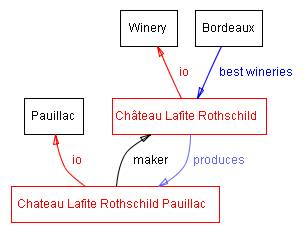
\includegraphics[width=0.5\linewidth]{Figures/fig_0.jpg}
    \caption{Example of a simple ontology in wine domain}
    \label{fig:wine_ontology}
\end{figure}
Fig.~\ref{fig:wine_ontology} depicts an example of an ontology in the wine domain; it represents wines, regions, producers.

\subsection{Classification}
In this section, we classify ontologies along multiple dimensions \cite{canfora2004ontologie}.
Firstly, ontologies can be classified according to the level of generality of the domain of discourse; specifically, from the most general to the most specific domains, as follows:
\begin{itemize}
    \item High-level ontologies describe very general concepts or common-sense knowledge such as space, time, objects, and actions. E.g., DOLCE ontology \cite{borgo2022dolce}.
    \item Domain ontologies describe the vocabulary, theories, and fundamental principles that govern a specific domain. E.g., tourism ontology \cite{tourismOntology2013}.
    \item Task ontologies: describe the vocabulary related to a specific task or activity, providing a specialization of the terms introduced in the high-level ontology. E.g., planning ontology \cite{taskOntologyPlanning}.
    \item Application ontologies describe concepts related to a specific domain or task and are often derived through a specialization of domain ontologies and task ontologies. E.g., OntoWeb \cite{ontoweb2002}.
\end{itemize}

Ontologies can differ in the level of formalism adopted. Therefore, they can be classified also as follows:
\begin{itemize}
    \item Highly informal ontologies are expressed in natural language, thus potentially leading to ambiguous definitions given the inherent ambiguity of natural language.
    \item Semi-informal ontologies are expressed in a rigid and structured form of natural language, improving clarity and reducing ambiguities.
    \item Semi-formal ontologies are expressed through formally defined artificial languages.
    \item Strictly formal ontologies are expressed with languages based on formal semantics.
\end{itemize}

A further classification can be made based on the expressiveness that the ontology aims to convey:
\begin{itemize}
    \item Controlled vocabularies are finite lists of terms representing the simplest possible notion of an ontology. A typical example is a catalogue that provides only terms with an unambiguous interpretation.
    \item Glossaries are lists of terms along their meanings expressed through natural language statements. Being primarily created for human use, they often consist of ambiguous statements that cannot be used by automated agents.
    \item Thesauri add semantics to glossaries by defining the relationships between terms (such as synonymy relations). Typically, they do not provide an explicit hierarchical structure, although this can be inferred from the specification of the terms.
    \item Informal Is-A hierarchies are ontologies in which generalization and specialization are achieved even though there is no strict "sub-class" hierarchy. They include various ontologies available on the Web.
    \item Formal Is-A hierarchies are ontologies in which concepts are organized according to a strict subclass hierarchy.
    \item Frames are ontologies in which concepts are described in terms of their characteristic properties. Inheritance relationships allow properties specified for general concepts to be inherited by more specific ones.
   \item Logic based ontologies represent knowledge in a formal structured manner, enabling reasoning and inference, e.g., classification and consistency check.
\end{itemize}

\subsection{Ontology Languages}
Ontology languages are formal languages designed to define and represent ontologies, which describe the structure of knowledge in a specific domain of interest \cite{ontolang_wiki}.
Knowledge in an ontology is divided into two components:
\begin{itemize}
    \item TBox (Terminological Box): defines the conceptual structure, including classes and properties, along with axioms that describe their relationships and constraints.

    \item ABox (Assertional Box): contains assertions about specific instances, describing which individuals belong to particular classes and how they relate to each other.
\end{itemize}
RDF (Resource Description Framework) is a framework used to describe graph data by using triples. Triples are used to define the ABox of an ontology, each triple has three components: 
$$
\langle subject, predicate, object\rangle
$$
The triple states that there is a relationship of type $predicate$ from the entity $subject$ to the entity $object$. Each triple component can be identified using a URI (Uniform Resource Identifier). The $object$ can be a literal or an URI while $subject$ and $predicate$ must be a URI.
For example, the triple:
\begin{lstlisting}
    <http://example.org/person/Alice> <http://example.org/knows> <http://example.org/person/Bob>.
\end{lstlisting}
it states that the resource identified by <http://example.org/person/Alice> knows (<http://example.org/knows>) a resource identified by <http://example.org/person/Bob>.
\begin{figure}[H]
    \centering
    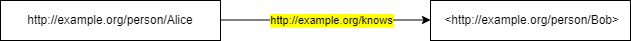
\includegraphics[width=0.9\linewidth]{Figures/fig_86.png}
    \caption{Relation between two individuals}
    \label{fig:86}
\end{figure}
Fig. \ref{fig:86} represents the RDF triple described before.

A more complex example is the following:
\begin{lstlisting}
    <http://example.org/person/Alice> <http://example.org/name> "Alice".

    <http://example.org/person/Bob> <http://example.org/name> "Bob".

    <http://example.org/person/Matt> <http://example.org/name> "Matt".

    <http://example.org/person/Alice> <http://example.org/knows> <http://example.org/person/Bob>.

    <http://example.org/person/Matt> <http://example.org/knows> <http://example.org/person/Alice>.
\end{lstlisting}
This examples involves three individuals: Alice (<http://example.org/person/Alice>), Bob (<http://example.org/person/Bob>) and Matt (<http://example.org/person/Matt>).
Each one has a name, associated with the relation <http://example.org/name> connecting the corresponding literal. Alice knows Bob, this is expressed by the triple: <http://example.org/person/Alice> <http://example.org/knows> <http://example.org/person/Bob>. Matt knows Alice, this is expressed by the triple <http://example.org/person/Matt> <http://example.org/knows> <http://example.org/person/Alice>.


\begin{figure}[H]
    \centering
    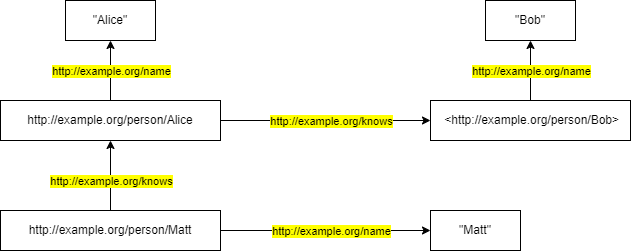
\includegraphics[width=0.9\linewidth]{Figures/fig_85.png}
    \caption{Relation between individual and name}
    \label{fig:85}
\end{figure}
Fig. \ref{fig:85} represents concepts described as an oriented labelled graph edge.
OWL is a family of knowledge representation languages for ontologies, the latest version OWL2, born in 2009, is used to build ontologies representing classes, properties, individuals, and data values that are stored as Semantic Web documents \cite{owl2}. 
OWL languages are based on DLs: a family of logic formalism derived from first order logics. Main OWL members (profiles) are:
\begin{itemize}
    \item OWL DL: based on Description Logics ($SHOIN$), it is designed to provide the maximum expressiveness possible.

    \item OWL Lite: simplified subset of OWL DL, based on $SHIF(D)$, with fewer constructs for simpler applications.

    \item OWL Full: based on a different semantics from OWL Lite or OWL DL, it is designed to be compatible with RDF.

    \item OWL 2: based on $SROIQ$: a more expressive extension of previous DLs ($SHOIN$).
\end{itemize}

In general, all OWL profiles define TBox: terminological component describing the interest domain. Interest domain is modelled through classes and properties.
\begin{table}[H]
    \centering
    \begin{tabular}{|>{\raggedright\arraybackslash}p{4cm}|>{\raggedright\arraybackslash}p{4cm}|>{\raggedright\arraybackslash}p{4cm}|}
        \hline
        Name & Syntax & Description \\ \hline
        Class & owl:Class & Represents a set of individuals \\ \hline
        Object Property & owl:ObjectProperty & Relates individuals to other individuals \\ \hline
        Data Property & owl:DatatypeProperty & Relates individuals to data values \\ \hline
        Individual & owl:NamedIndividual & Represents an instance of a class \\ \hline
    \end{tabular}
    \caption{Main OWL2 constructs}
    \label{table:t_2_1}
\end{table}
Table \ref{table:t_2_1} contains the main constructs in OWL2.
The main reason for choosing OWL2 is its capacity to support automatic reasoning, inferring new knowledge starting from what is represented in the ontology.
Reasoning is important to verify the consistency of the ontology, determine subsumption relations between concepts, check whether an individual belongs to a certain class and retrieve informations.
For instance, suppose we have an ontology that defines the concept of "Animal" and its subclasses, such as "Mammal" and "Bird". If we also define that "Cat" is a subclass of "Mammal", and we have an individual "Whiskers" that belongs to the "Cat" class, a reasoner can automatically infer that "Whiskers" is also a "Mammal" and an "Animal", even if these relationships were not explicitly declared.

One important aspect is the adoption of the Open World Assumption (OWA), which implies that the absence of information does not imply its falsehood so if data are not declared we do not have informations to establish its truth.
This is useful in the semantic web where the knowledge is distributed across different sources and it is impossible to have access to all possible informations.

SPARQL is a semantic query language that allows to retrieve and manipulate data stored in RDF format.
It is based on triple patterns, i.e., statements consisting of a subject, predicate, and object, which resemble RDF triples. These triples are used to define queries that match specific data in RDF.
An example of SPARQL query is the following:
\begin{lstlisting}
PREFIX foaf:   <http://xmlns.com/foaf/0.1/>
SELECT ?name ?mbox
WHERE
  { ?x foaf:name ?name .
    ?x foaf:mbox ?mbox 
}    
\end{lstlisting}
This SPARQL query selects and returns the names (\texttt{?name}) and email addresses (\texttt{?mbox}) of entities (\texttt{?x}) that have a \texttt{foaf:name} and \texttt{foaf:mbox} property defined in the FOAF vocabulary. 

SWRL (Semantic Web Rule Language) is a language for semantic web that can be used to express logic rules, combining OWL DL with a subset of Datalog. Rules are of the form of an implication between an antecedent (body) and a consequent (head). The intended meaning can be read as: whenever the conditions specified in the antecedent hold, then the conditions specified in the consequent must also hold \cite{swrl_wiki}. An example of SWRL rule is the following:
\begin{lstlisting}
hasParent(?x1,?x2) ∧ hasBrother(?x2,?x3) -> hasUncle(?x1,?x3)
\end{lstlisting}
This SWRL rule states that if $?x1$ has a parent $?x2$, and $?x2$ has a brother $?x3$, then $?x3$ is the uncle of $?x1$. It infers family relationships in an ontology, allowing automatic reasoning about uncles based on parents and siblings.
SWRL extends OWL enabling advanced inferences but a drawback is that it can be computationally expensive and rules are not executable in all reasoners.

\subsection{Ontology Repositories}
Ontology repositories facilitate the discovery of ontologies and thus their reuse, main repositories are:
\begin{itemize}
    \item W3.org \footnote{https://www.w3.org/wiki/Lists\_of\_ontologies}: a curated list of ontologies covering various domains, maintained by W3C.

    \item DBpedia \footnote{https://archivo.dbpedia.org/list}: a repository of linked data ontologies extracted from Wikipedia, enabling semantic web applications.

    \item AgroPortal \footnote{https://agroportal.lirmm.fr/ontologies?search=o}: a platform hosting agricultural and food-related ontologies for data interoperability.

    \item BioPortal \footnote{https://bioportal.bioontology.org/ontologies}: a repository of biomedical ontologies providing standardized vocabularies for health and life sciences.

    \item LOV (Linked Open Vocabularies) \footnote{https://lov.linkeddata.es/dataset/lov/}: a repository of linked data vocabularies, facilitating ontology reuse and interoperability.


    \item OntoHub \footnote{https://github.com/ontohub/ontohub}: a web-based repository for distributed ontologies, models and specifications.
\end{itemize}
Any user can contribute to these repository by submitting a new ontology or commenting and suggesting improvements to existing ontologies.



\section{Ontology Engineering}
\label{section:2_2_ontology_engineering}
Ontology Engineering is the discipline that focuses on the design, development, and management of ontologies. It involves various activities such as ontology specification, knowledge acquisition, conceptualization, formalization, implementation, evaluation, maintenance, and documentation. The goal is to create structured, machine-readable knowledge representations that facilitate interoperability, reasoning, and knowledge sharing. This process relies on formal languages like OWL and RDF and employs tools such as Protégé.\cite{falquet2011introduction}
In this section, we describe the main state-of-art techniques and methodologies in ontology engineering. Finally we discuss some ontology design patterns that can be reused in the ontology design.
\subsection{Requirements Definition and Conceptualization}
The definition of requirements and the subsequent conceptualization are two fundamental tasks in ontology engineering.
They aim at establishing the objectives and scope of the ontology, and the constructs within it, respectively.
To define the scope and the requirements that the ontology should be able to address, Competency Questions (CQs) stand for the state-of-the-art approach.
They are questions written in natural language that the ontology should be able to answer \cite{malheiros2013method}.

For instance, in the development of an ontology for noise pollution monitoring \cite{espinoza2020using}, the following CQs have been defined:
\begin{table}[H]
    \centering
    \begin{tabular}{|>{\raggedright\arraybackslash}p{1cm}|>{\raggedright\arraybackslash}p{6cm}|>{\raggedright\arraybackslash}p{6cm}|}
        \hline
        Id & Competency question & Answer \\ \hline
        CQ1 & Which is the measured noise level in a specific moment and location? & The detected noise level during April in location with coordinates 40.42, – 3.69, 648 is 67.4 dB. \\ \hline
        CQ2 & Which is the location of a specific measurement station? & The location of the measurement station “Paseo de Recoletos” is 40.42, – 3.69, 648 (Longitude, Latitude, Altitude) \\ \hline
        CQ3 & In which day interval the noise level has been detected? & The noise level Ld has been detected in the time interval between 07:00 to 19:00. \\ \hline
        CQ4 & Which was the last calibration sensor date? & The datetime, for example, 2017-04-21T14:00:00+01:00 \\ \hline
    \end{tabular}
    \caption{Competency Questions noise pollution ontology}
\end{table}
Each CQ must correspond to a natural language answer that "simulates" the response provided by the ontology.
CQs are translated into SPARQL queries in order to be executed on the ontology.
Once defined, CQs can be used for evaluating an ontology.

The conceptualization (or design) of the ontology aims at defining the classes, the relationships among them, and the individuals.
There are three approaches to conceptualization:
\begin{enumerate}
    \item Top-down development process starts with the definition of the most general concepts in the domain and subsequent specialization of the concepts.
    \item Bottom-up development process starts with the definition of the most specific classes, the leaves of the hierarchy, with subsequent grouping of these classes into more general concepts.
    \item Hybrid development process is a combination of the top-down and bottom-up approaches: we define the most salient concepts first and then generalize and specialize them appropriately.
\end{enumerate}

\subsection{Methodologies}

\paragraph{METHONTOLOGY}
METHONTOLOGY \cite{fernandez1997ontological} proposes a structured method consisting of six steps:  
Firstly, the specification phase aims at producing the ontology specification document, outlining the main requirements and the scope of the ontology.
It can be informal, semi-formal, or formal, and is written either in natural language or using CQs.
Next, the \textsf{knowledge acquisition} phase involves gathering all relevant knowledge related to the domain. 
It can be performed based on various techniques, such as text analysis, brainstorming, interviews, and reviewing existing similar ontologies.

The \textsf{conceptualization} phase follows, where the acquired knowledge is organized into a conceptual model.
During the \textsf{integration} phase, the methodology encourages reusing and integrating existing ontologies rather than developing new ones from scratch. 
This step is crucial for ensuring consistency and coherence, as it involves checking libraries of ontologies to find definitions of terms that match the semantics identified in the conceptualization phase.
The \textsf{implementation} phase is where the actual construction of the ontology takes place.
Finally, the \textsf{evaluation} phase ensures the quality and correctness of the ontology.
This step involves both verification, to confirm that the ontology is semantically sound, by using a reasoner, and validation.

The methodology has the following advantages: 
\begin{itemize}
    \item It proposes the use of an evolutionary prototype life cycle, which allows definitions to be modified, added or removed at any time.

    \item It encourages the reuse of already existing ontologies, which can speed up development and ensure consistency with other projects. 
\end{itemize}

However, it also has disadvantages:
\begin{itemize}
    \item The methodology is very detailed and rigorous, which can be time and resource consuming, especially for smaller projects, it may be excessive compared to the needs of the project.

    \item The methodology can be complex to master for those without experience in ontology development, as it requires familiarity with several specific techniques and tools.

    \item The methodology has been developed in 1997, making it outdated by today standards. Since its creation, there have been significant advancements in both ontology engineering and related technologies, such as the Semantic Web, Linked Data, and agile methodologies.

    \item The methodology was created before the widespread adoption of agile development practices, which are now a common approach in software and ontology engineering. This makes it less flexible for fast-paced, iterative development environments.
\end{itemize}

\paragraph{NeOn}
Another proposed methodology is the NeOn methodology \cite{neon1,neon2}, which provides guidance for all key aspects of the ontology engineering process.
The concepts underlying this methodology are: scenarios, collaborative ontology development, reuse of ontological and non-ontological resources and evolution of networked ontologies. 

The ontology engineering is based on nine scenarios:
\begin{itemize}
    \item Scenario 1: from specification to implementation The ontology network is developed from scratch, engineers should specify ontology requirements and search for potential resources to be reused. 

    \item Scenario 2: reusing ontological resources Engineers reuse ontological resources, ontology modules and ontology statements to build ontology networks. 

    \item Scenario 3: reusing and re-engineering ontological resources Ontology engineers reuse and re-engineer ontological resources

    \item Scenario 4: reusing and merging ontological resources This scenario arises when several ontological resources in the same domain are selected for reuse, and engineers wish to create a new ontological resource with the selected resources

    \item Scenario 5: reusing, merging and re-engineering ontological resources Ontology engineers reuse, merge, and re-engineer ontological resources. 
    This scenario is similar to Scenario 4, but here engineers decide to re-engineer the set of merged resources

    \item  Scenario 6: reusing ontology design patterns Ontology engineers access repositories to reuse design patterns

    \item Scenario 7: ontology engineers access repositories to reuse design patterns Ontology engineers restructure (e.g., modularize, prune, extend, and/or specialize) ontological resources to be  integrated in the ontology network. 

    \item Scenario 8: localizing ontological resources Ontology engineers adapt an ontology to other languages and culture communities, thus obtaining a multilingual ontology.

\end{itemize}
The scenarios presented are not a rigid workflow, they are more like a variety of pathways for developing ontologies and they cover commonly occurring situations, for example, when available ontologies need to be re-engineered, aligned, modularized, localized to support different languages and cultures, and integrated with ontology design patterns and non-ontological resources, such as folksonomies or thesauri\cite{suarez2011neon}.

The \href{http://neon-project.org/nw/Welcome_to_the_NeOn_Project.html}{Neon project} offers to engineers a tool called \href{http://neon-toolkit.org/wiki/Main_Page.html}{NeOn toolkit}: an open-source multi-platform ontology editor which supports OWL2 and features basic editing and visualization functionalities \cite{erdmann2011overview}.

\begin{figure}[H]
    \centering
    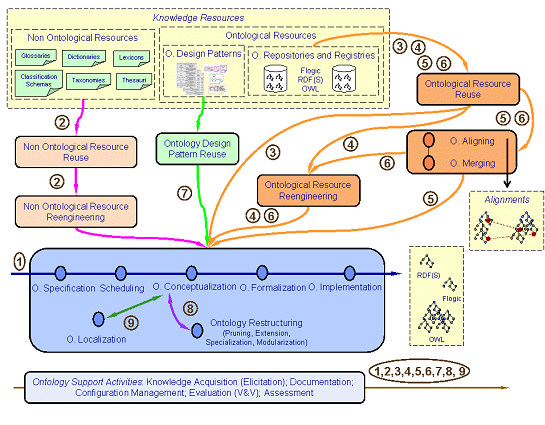
\includegraphics[width=0.5\linewidth]{Figures/fig_2.png}
    \caption{NeOn methodology scenarios}
    \label{fig:2}
\end{figure}
Fig.~\ref{fig:2} represents the different scenarios in the NeOn methodology.
The NeOn methodology has the following advantages:
\begin{itemize}
    \item It identifies nine different scenarios for building ontology networks, which can be combined depending on the project’s needs, this contrasts with more rigid methodologies like METHONTOLOGY.

    \item It supports the reuse and re-engineering of both ontological and non-ontological resources, which can save time and effort by leveraging existing knowledge bases, reducing the need to build everything from scratch.

    \item By basing its structure on real use cases and generalizing from them, the NeOn methodology covers practical needs encountered in ontology development projects.
\end{itemize}
However, NeOn has the following disadvantages:
\begin{itemize}
    \item The flexibility and comprehensive nature of the methodology can make it more complex to apply, especially for teams without significant prior experience in ontology development. 

    \item Although NeOn is designed for building large-scale networks, the actual process of merging and aligning different ontologies can be challenging, especially when ontologies come from diverse sources with differing structures and standards.

    \item The methodology is meant to be technology-independent, in practice, it may require specific tools to implement the processes effectively, and these tools might not always be accessible or easy to use for all teams.
\end{itemize}

\paragraph{XD methodology}
While the NeOn methodology is scenario-based, the eXtreme Design (XD) methodology \cite{presutti2009extreme} is based on a sequence of tasks inspired by the principles of agile development in software engineering.
XD involves the stakeholders in order to gather complete requirements without making incorrect assumptions.
This interaction is useful for defining CQs and user stories that detail the use of the ontology, supported by contextual statements that make implicit knowledge explicit.
The principles of XD not only focus on the customer, but also provide clear guidelines to engineers regarding the design and organization of work.
In particular, the design must be modular and task-oriented, focusing on the specifications defined in the CQs.
The CQs are used in the development of unit tests during the testing phase, verifying the compliance of the ontology with the customer stories.
Tests are generally conducted using SPARQL queries that encode the CQs.
Throughout the development phase, the engineers are organized according to the pair design, where the design team is divided into pairs that must collaborate, by sharing knowledge.
Based on the illustrated principles, XD defines the following tasks: 
\begin{itemize}
    \item Task 1. Get into the project context: the development process begins by aligning the engineers and domain experts, who may have different backgrounds and terminologies. The goal is twofold: to familiarize the customer with the project's methods and tools, and to provide the engineers with an understanding of the problem, scope, and initial terminology as well as establishing a collaborative environment for sharing documentation and discussing modelling issues.

    \item Task 2. Collect requirement stories: the customer writes stories starting from real scenarios in order to provide examples of the typical facts that should be stored in the ontology.

    \item Task 3. Select a story that has not been treated yet: each pair of engineers selects a story to focus on for the next iteration for releasing an ontology module. They create a new wiki page with the story's title and content based on the information from the card.

    \item Task 4. Transform the story into CQs: create a sequence of CQs, this task involves customer for having feedback/clarifications.

    \item Task 5. Match the CQ to use cases: identify candidate Content Patterns (CPs) (a specific type of ontology design patterns, see Sect.~\ref{subsection:2_2_ontology_design_patterns}) based on the CQs that express part of the ontology to be modelled. Matching can be done with tool support, such as keyword-based searching, or manually by engineers familiar with available CPs.

    \item Task 6. Select the CPs to reuse: select which of those patterns should be used for solving the modelling problem.

    \item Task 7. Reuse and integrate selected CPs: apply typical operations for CPs i.e. import, specialization, and composition. 

    \item Task 8. Test and fix: validate the module by ensuring it aligns with the CQs just modelled. This process involves several steps: first, the CQ is transformed into a unit test, such as a SPARQL query, then, the module is populated with sample data based on the story, and the test is run. If the result isn't as expected, the module is revised and the test is rerun until it passes and once all tests linked to the story have been successfully completed, the engineers can move on to the next task. If any CQ remains unaddressed, they return to an earlier task to make adjustments.

    \item Task 9. Release module: release an ontology module having an URI shared with the whole team and on web repositories.

    \item Task 10. Integrate, test and fix: integrate the module with the other modules that constitute the ontology.
\end{itemize}

Once the eleven tasks have been completed, the release of the new version of the ontology takes place.
The XD methodology has the following advantages:
\begin{itemize}
    \item The methodology supports collaboration and modular ontology development, allowing teams to work on different parts of the ontology in parallel, which is especially useful for large and distributed projects.

    \item It employs a test-driven approach, where CQs and contextual statements serve as the basis for unit testing the ontology, ensuring that each component meets its intended purpose before moving forward.

    \item The methodology emphasizes constant interaction with domain experts and stakeholders to ensure that the ontology meets the intended use and requirements. This minimizes assumptions and ensures that implicit knowledge is captured.
\end{itemize}
However, there are also disadvantages:
\begin{itemize}
    \item The methodology's iterative, test-driven nature may be overkill for smaller ontology projects, where a simpler, more direct approach could be more efficient.

    \item Effective use of XD relies on the availability of supporting tools, such as the NeOn Toolkit and its XD plugin. While these tools are valuable, they may limit accessibility if they are not well-maintained or widely available.
\end{itemize}

\paragraph{LOT methodology}
The Linked Open Terms (LOT) methodology \cite{poveda2022lot} is a lightweight industrial-oriented methodology for ontology engineering.
The methodology is compatible with software engineering methodologies; indeed, it is inspired by the agile methodology.
\begin{figure}[H]
    \centering
    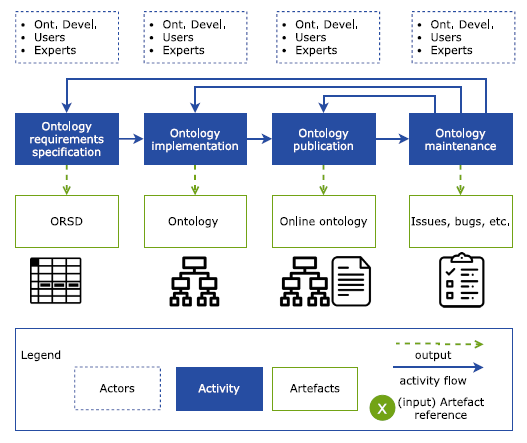
\includegraphics[width=0.7\linewidth]{Figures/fig_3.png}
    \caption{LOT methodology base workflow}
    \label{fig:lot-workflow}
\end{figure}

Fig.~\ref{fig:lot-workflow} describes the ontology development lifecycle with four stages: requirements specification, implementation, publication, and maintenance, involving collaboration between ontologists, developers, users, and experts.
Each stage outputs artefacts (e.g., ORSD, ontology, online ontology) that flow into subsequent phases for iterative refinement and usage.

This phase aims at defining the domain of interest, the goal of the ontology and the implementation language.
In detail, there are seven steps as described below.
Initially, use case specifications are created in collaboration with domain experts, users, and ontology engineers.
These use cases describe scenarios in which the ontology will be utilized and are expressed in natural language.
Next, data exchange identification is carried out, where the necessary documentation and resources related to the domain are gathered and compiled into a set of documents.
The purpose and the scope of the ontology are then identified with input from users and domain experts.
The purpose clarifies the reason for creating the ontology, while the scope defines the aspects of the domain that will be represented.

Subsequently, a set of functional ontological requirements is proposed, often in the form of CQs or natural language statements.
These requirements outline what the ontology should be able to answer and represent. 
Ontology experts then review these functional requirements to ensure their correctness and completeness, addressing any ambiguities and verifying consistency with the defined purpose and scope.
Following this, the Ontology Requirements Specification Document (ORSD) is formalized.
This document consolidates all the information, CQs, and functional requirements defined in the earlier phases, serving as a comprehensive reference for the ontology engineering. 
In some cases, an optional activity is conducted where the functional ontology requirements are further formalized into test cases, expressed in SPARQL queries.
This step helps in validating that the ontology meets the specified requirements through structured testing.

In this phase, the ontology is implemented using a formal language.
Firstly, it involves the conceptualization, which aims at defining the constructs in the ontology.
Next, the encoding phase aims at actually implementing the ontology using an implementation language; in this phase, is useful to take into account other similar ontologies that could be reused.
Once the whole ontology is completed, it can be evaluated according to different evaluation criteria.

In this phase, the ontology is published online, making it accessible and searchable by users. 
Before publishing the ontology online, it is necessary to identify the version to be released, document the ontology using human-readable HTML pages, and finally publish the ontology online according to the W3C guidelines \cite{ontology_online}.

The last step is the ontology maintenance.
In this phase, once the ontology is published online, bug detection is performed.
Moreover, the ontology can be updated according to new requirements.

Despite being introduced recently, the LOT methodology has been widely applied successfully, both in research and in the industrial field.
In the industrial and manufacturing sector, the ontology SAREF4INMA \cite{de2020saref4inma} has been developed to describe equipment, materials, products, factories and manufacturing processes in a structured way. 
The industry is not the only sector where an ontology developed with the LOT method can be applied.
In Spain, specifically in Madrid, an ontology has been developed to represent the Bus Public Transport system \cite{ruckhaus2023applying}. 
The ontology represents information on lines, routes, journey patterns and their timetables, stops on each route, information on expected bus arrival times for each stop, and information on incidents that may affect the bus routes and their journeys.
Still in Spain, the LOT methodology has been successfully used in the development of a noise pollution ontology \cite{espinoza2020using}.
The ontology integrates data from Internet of Things (IoT) sensors in the city and establishes semantic relationships between them.

The LOT methodology has been used also in AI research field, the HALO ontology \cite{nananukul2024halo} has been creating for representing hallucinations in LLMs.
The ontology represents LLMs, hallucinations, prompts and responses.
The ontology consists of two modules and was created from a dataset of 40 known prompts designed to generate hallucinations.
Each prompt was given as input to three LLMs: ChatGPT, BARD, and Claude.
\begin{figure}[H]
    \centering
    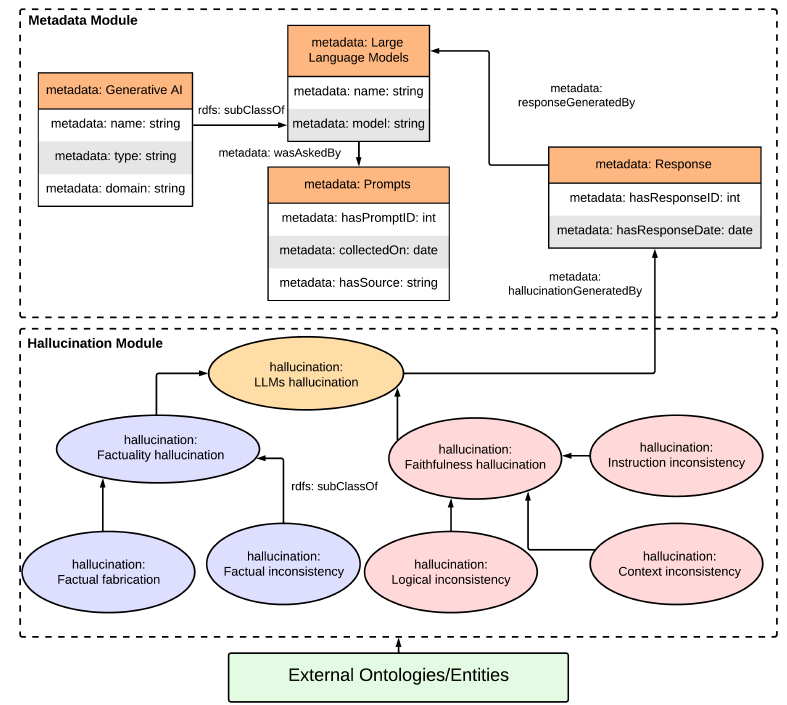
\includegraphics[width=0.7\linewidth, height=8cm]{Figures/fig_4.png}
    \caption{HALO ontology}
    \label{fig:halo}
\end{figure}
Fig. \ref{fig:halo}

The LOT methodology has the following advantages:
\begin{itemize}
    \item The LOT methodology is designed to be lightweight and agile, which allows for faster iterations and easier integration with software development practices and it is particularly well-suited for projects that need rapid, iterative development.

    \item It offers flexibility by combining various techniques (CQs, natural language statements ...) to define requirements and allows for different levels of formality depending on the project.

    \item Many open source ontologies have been developed successfully using the LOT methodology, e.g., the public transport ontology.
\end{itemize}
But, the LOT methodology has two disadvantages:
\begin{itemize}
    \item LOT encourages the reuse of existing ontologies, but this can be challenging due to the potential inconsistencies and heterogeneity of reused ontologies. However, the methodology does not fully address how to resolve these issues.

    \item The emphasis of LOT on formal validation processes (such as the use of SPARQL queries) may not be sufficient for certain complex domains or non-technical stakeholders.
\end{itemize}

% vediamo se tenerla
\subsection{Ontology Engineering using Large Language Models}
The methodologies analysed for ontology design involve users, domain experts, and ontology engineers, but do not include the use of advanced tools based on artificial intelligence, such as LLMs. The study "From human experts to machines: An LLM supported approach to ontology and knowledge graph construction" \cite{kommineni2024human} introduces a semi-automatic pipeline for the construction of knowledge graphs. There are six phases in the proposed pipeline.
The process begins with the data collection phase, which does not involve the use of large language models (LLMs). Instead, domain experts generate a dataset and a set of publications relevant to the topic under study.
In the next phase, known as competency question (CQ) generation, ChatGPT-3.5 is utilized to create competency questions. These questions are designed to describe the data collected in the previous phase at an abstract level. Domain experts provide inputs to the LLM to generate these questions, which are then evaluated by two domain experts to ensure their relevance and accuracy. Following this, the ontology creation phase is initiated. It builds on the competency questions generated earlier. This phase involves two steps: in the first step, a prompt is created that includes a competency question, the expected output, and a set of instructions. In the second step, the LLM is provided with a basic ontology structure containing the concepts and relationships derived from the competency questions.
The CQ answering phase involves applying text processing techniques to extract answers to the competency questions. These answers are used to enrich the ontology and provide a deeper understanding of the dataset.
During the knowledge graph (KG) construction phase, the competency questions, their answers, and the ontology generated by the LLM are combined and provided as input to the LLM. The prompt for this phase focuses on extracting entities, relationships, and concepts and mapping them onto the ontology, thereby creating a comprehensive knowledge graph.
Finally, in the evaluation phase, the LLM evaluates the competency questions and the constructed knowledge graph by comparing them to a ground truth generated by human evaluators. The LLM assigns a score based on the alignment of the generated knowledge graph with the human-generated ground truth.
The presented method enabled the creation of a fairly complex ontology consisting of 45 classes, 41 relations, and 365 axioms. However, it required significant computational resources, as an 80GB NVIDIA A100 GPU machine was used. 
Another approach for ontology learning using large language models is NeOn-GPT \cite{fathallah2024neon}. Starting from the NeOn methodology, the methodology is converted to a series of prompts to ChatGPT-3.5, these prompt are created using prompt engineering techniques and they are used first to generate ontology specification and competency questions. ChatGPT-3.5 is used also to generate a conceptual model of the ontology in the form of subject-relation-object triples and to generate implementation code. Once the code is generated, there is the syntax validation using the RDFLib python library \cite{rdflib} and the consistency check in order to check logical inconsistencies. The final step is the pitfall resolution for checking circular axioms and missing disjointedness using OODPs API. The presented methodology is an evolution of the NeOn methodology, in which all tasks traditionally performed by the engineer are delegated to ChatGPT. This includes identifying requirements, writing competency questions, conceptualizing, and implementing the ontology.%\\
ChatGPT can be used not only for the creation of ontologies but also for the creation of more complex knowledge graphs, specifically Hyper-Relational Knowledge Graphs, as discussed in the study "Construction of hyper-relational knowledge graph using pre-trained large language models" \cite{datta2024construction}. Hyper-relational knowledge graphs unlike the normal knowledge graphs incorporate additional qualifiers or attribute-value pairs \cite{hyper}, in the study starting from HyperRED dataset, a dataset about different topics , the hyper relational knowledge graph is built including in prompts the data from the dataset. Prompts are generated using Chain-of-Thoughts prompt engineering technique (CoT) and in order to evaluate the result generated, BERTScore is choose as a metric. The results obtained were not satisfactory, as the other algorithm(CubeRE)for extracting hyper-relational information was not surpassed.
In general, large language models have shown promising potential  in automating and enhancing the processes of ontology and knowledge graph construction replacing the ontology engineer in different tasks.

\newpage
\subsection{Ontology Design Patterns}
\label{subsection:2_2_ontology_design_patterns}
In ontology engineering, Ontology Design Patterns (ODPs) \cite{odps} are a powerful approach for addressing recurring problems in the design of ontologies \cite{hitzler2016ontology}.

An OP is a modelling solution for solving a recurrent ontology design problem \cite{gangemi2009ontology}.
These patterns encapsulate best practices, enabling ontology engineers to draw from proven solutions when confronted with similar challenges and enabling them to optimize time and costs during the design. 

In \cite{falbo2013ontology} there are five types of ODPs:
\begin{enumerate}
    \item Structural ODPs

    \item Reasoning ODPs

    \item Correspondence ODPs

    \item Presentation ODPs

    \item Lexico-Syntactic ODPs

    \item Content ODPs
\end{enumerate}
We describe each type in detail below.

Structural ODPs are high-level modelling solutions that address architectural and logical challenges in ontology design.
They include two main subtypes:
\begin{itemize}
    \item Logical ODPs: these are combinations of logical constructs that resolve expressivity issues in ontology languages. They operate independently of specific content domains and are designed to bridge gaps where a representation language lacks built-in constructs. For example, Logical ODPs help model n-ary relations in OWL, which only supports binary relations.

    \item Architectural ODPs: these patterns influence the overall shape and structure of an ontology. They can be internal, focusing on consistent use of Logical ODPs within an ontology or external, involving meta-level constructs like modular networks connecting multiple ontologies.
\end{itemize}

Reasoning ODPs are applications of Logical ODPs specifically designed to achieve certain reasoning outcomes.
Examples of Reasoning ODPs include classification, subsumption, inheritance, materialization, de-anonymization, and others.
When applied to an ontology, Reasoning ODPs provide insights into the state of the ontology and enable a system to determine the type of reasoning required to perform tasks such as queries, evaluations, and more.

Correspondence ODPs are a type of ODP that focuses on addressing relationships and transformations between ontologies or between ontologies and non-ontological resources.
They are divided into two main types:
\begin{itemize}
    \item Re-engineering ODPs: provide guidelines for transforming ontological and non-ontological models, such as database schemas or thesauri, into ontologies. 

    \item Mapping ODPs: These focus on creating semantic associations between elements of different ontologies without altering their structure. They help define equivalence, containment, and overlap relations as well as their negative counterparts.
\end{itemize}

Presentation ODPs focus on improving the usability and readability of ontologies from a user perspective.
They serve as best practices to enhance reusability by making ontologies easier to evaluate and select.
Key types include:
\begin{itemize}
    \item Naming ODPs: provide conventions for naming ontology elements (classes, properties, files, namespaces). These ensure consistency and improve human readability and understanding.

    \item Annotation ODPs: define annotation properties or annotation property schemas that add metadata to ontology elements, enhancing their understandability and context.
\end{itemize}
For example, a Naming OP might recommend using the base URI of the publishing organization (e.g., http://www.example.org/ontologies/) to ensure clarity and consistency.
Annotation ODPs could include descriptive metadata, such as the purpose or scope of a class.
These patterns are essential for supporting effective reuse, adaptation, and user accessibility in diverse domains.

Content Patterns (CPs) are conceptual ODPs that address domain-specific modelling issues in ontologies.
Unlike Logical ODPs, which are general and conceptualization-independent, CPs focus on solving content problems by proposing patterns for modelling domain-specific classes and properties.
CPs are reusable through specialization, extension, or composition and impact only the ontology regions addressing particular modelling problems.
Although language-independent in theory, CPs require implementation for practical reuse, often using OWL.

Lexico-Syntactic ODPs are linguistic structures or patterns composed of specific word types arranged in a particular order.
These patterns allow for generalization and enable the extraction of conclusions about the meaning they convey.
They are particularly useful for linking basic Logical and Content ODPs with natural language sentences, such as in educational or instructional contexts.

A more practical approach to ODPs is given by the Modular Ontology Design Library (MODL) \cite{shimizu2019modl}.
MODL is a curated, well-documented, and structured collection of ODPs implemented in OWL designed to support modular ontology design.
This library promotes the FAIR (Findable, Accessible, Interoperable, and Reusable) guiding principles for scientific data management and stewardship by addressing challenges like ontology reusability and interoperability.
The library includes five categories of patterns: meta-patterns, organization of data, space-time movement, agents and roles, description, and details.
MODL offers patterns for dynamic processes, complex roles, and detailed relationships like part-whole hierarchies.
Its diversity ensures modularity and expressiveness for both general and domain-specific needs.

\section{Large Language Models}
\label{section:2_3_llms}
\subsection{Introduction and Classification}
LLMs, as seen before, are capable of supporting ontology engineering.
More broadly, this revolutionary AI technology is applied to various tasks across diverse domains, mainly because of their remarkable performance and versatility.
A LLM is a large-scale, pre-trained statistical LM based on neural networks; it is capable of natural language generation, which can be used to frame a large variety of Natural Language Processing (NLP) tasks \cite{zhao2023survey}.
LLMs are trained on a vast amount of training data in order to predict the next word in a given sequence of words of any length, language and even including mathematical formulas and code \cite{zhao2023survey}.
LLMs are able to execute different heterogeneous tasks thanks to an underlying complex neural-network, with transformer architecture being the most advanced.
Introduced in the 2017 by the seminal paper ``Attention Is All You Need'' \cite{vaswani2017attention}, the transformer architecture is composed by two parts:
\begin{enumerate}
    \item Encoder: a multilayer component where each layer consists of a multi-head self-attention mechanism and a position-wise fully connected feed-forward network.
    
    \item Decoder: a multi-layer component that processes the encoder's output. Each layer is based on a modified self-attention mechanism that prevents future positions from influencing past positions, ensuring autoregressive property.
\end{enumerate}
\begin{figure}[H]
    \centering
    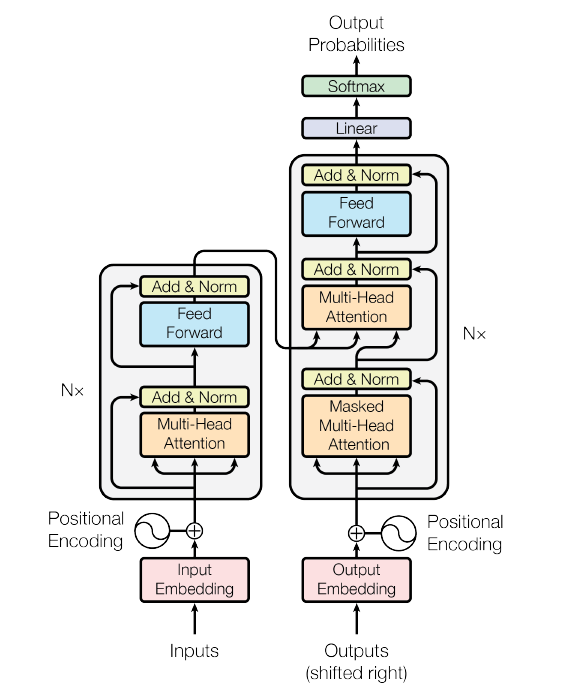
\includegraphics[width=0.5\linewidth]{Figures/fig_17.png}
    \caption{Transformer architecture}
    \label{fig:17}
\end{figure}
Fig.~\ref{fig:17} depicts the transformer architecture with with the encoder (on the left) and the decoder (on the right).
Two different variants of the transformer architecture have been adopted:
\begin{itemize}
    \item Encoder-Decoder: processes inputs through the encoder and passes the intermediate representation to the decoder to generate the output \cite{encoder_medium}.

    \item Decoder-only: does not have an encoder and it uses a decoder in order to generate tokens, each token depends on the previous sequence \cite{uniteai_decoder}.

    \item Encoder-only: does not have a decoder and it processes the entire sequence simultaneously generating contextualized representations for each token\cite{ewer2024entp}.
\end{itemize}

The simplicity and versatility of the decoder-only architecture allows for reaching extremely large scale (billions of parameters and hundreds of gigabytes of training data).
Such an unprecedented scale endowed LLMs with the so-called emerging abilities.
They made LLMs able to solve a large variety of tasks with remarkable performance with no need for additional re-training or fine-tuning, but simply needing to be prompted.
Indeed they are also called general purpose LLMs or Foundation Models.
Such emerging abilities include:
\begin{itemize}
    \item Instruction following: the ability of an LLM to execute commands and respond coherently to user instructions.

    \item In-context learning: the capability to learn and generalize from examples provided within the same interaction session, without updating the model’s weights.

    \item step-by-step problem solving: the ability to break down complex problems into simpler steps, following a structured process to reach a solution.
\end{itemize}
Such abilities constitute the basis for the definition of effective prompts.
Despite being less general than GPT, also BERT and T5 are often considered Foundation Models as they have represented crucial milestones in the development of LLMs.
Moreover, for classification (summarization) tasks, BERT (T5) can still outperform GPT and other very large decoder-only LLMs.

\subsection{State-of-the-art Large Language Models}
General purpose LLMs are capable of performing a wide variety of tasks.
In this section, we will analyse and discuss the following state-of-the-art general purpose LLMs:
\begin{itemize}
    \item GPT
    \item BERT
    \item PaLM
    \item LLaMA
    \item T5
    \item BLOOM
    \item Mistral
\end{itemize}

The Generative Pre-trained Transformer (GPT), released by Open AI, is actually the most advanced and powerful LLM available to users.
In two months, it gained over than 100 million of users, making it the fastest-growing consumer software application in history \cite{achiam2023gpt}.
GPT is a decoder-only LLM.

Since its first version, GPT-1 released in 2018, the model has represented a step forward in AI.
GPT-1 has 117 million parameters and is trained on the BookCorpus dataset.
The model has been improved in 2019 with the next version GPT-2, which has 1.5 billions of parameters and is trained on WebText dataset with 8 millions of documents \cite{radford2019language}.
In 2020, OpenAI has released GPT-3, which has 175 billions of parameters and is trained over one trillion of documents.
The latest version of GPT is GPT-4; it is a multimodal model, i.e., it can take as input both images and text and generate a response consisting of both images and text.
Despite the continuous evolution and the billions of parameters of the model, it is still subject to issues, including hallucinations \cite{achiam2023gpt}.
In general, an hallucination is a response generated by an AI model that contains false or misleading information presented as a fact. An example of hallucination is the following:
\begin{lstlisting}
Prompt: Who won the 2024 Formula 1 constructors world championship?
Response: The Redbull team won the Formula 1 constructors world championship in 2024
\end{lstlisting}
The response is wrong because McLaren team won in 2024 the Formula 1 constructors world championship in 2024.
Another example is:
\begin{lstlisting}
Solve the equation: 3x - 11 = 5
Response: x = 4
\end{lstlisting}
The response is wrong because the correct result is $5.33$ given by $x = \frac{11+5}{3}$.

GPT is a proprietary LLM, so its parameters and training set are not publicly available.
GPT has been made available to the public as a web application called ChatGPT and represented in Fig.~\ref{fig:18}.

\begin{figure}[H]
    \centering
    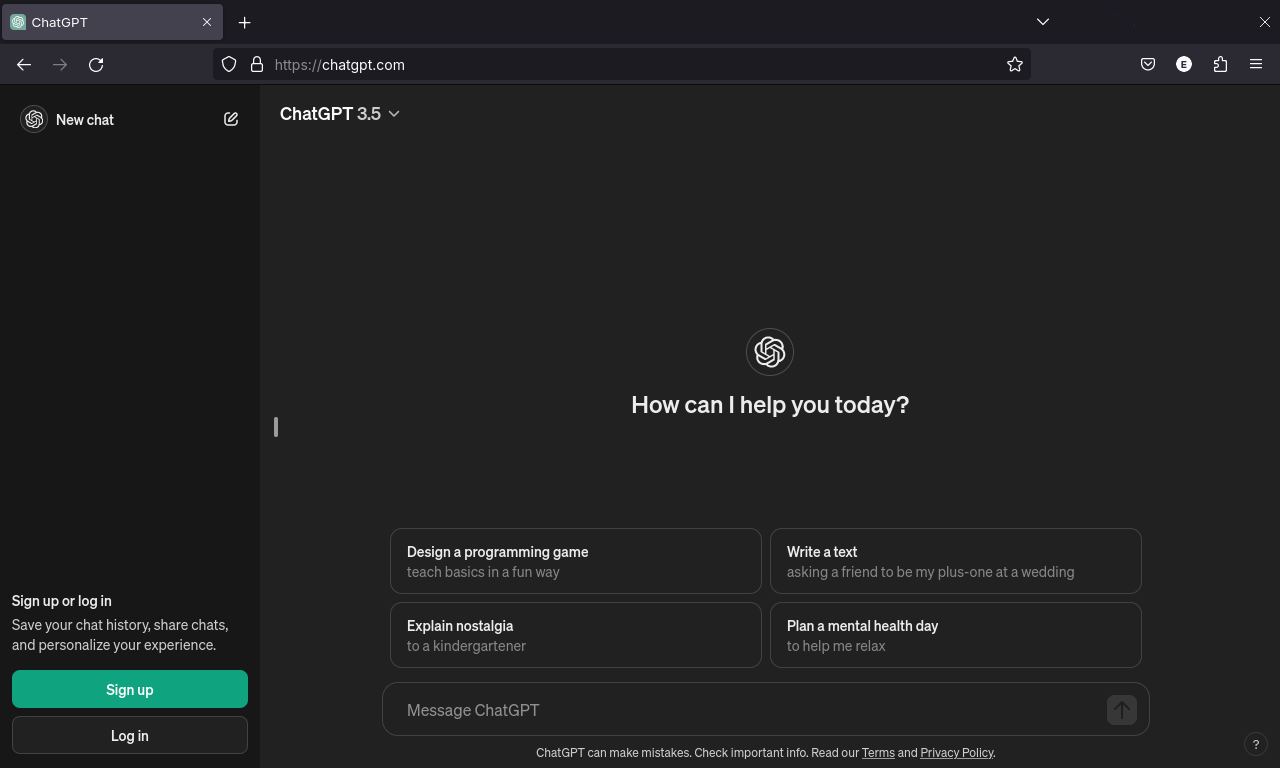
\includegraphics[width=0.9\linewidth]{Figures/fig_18.png}
    \caption{ChatGPT interface}
    \label{fig:18}
\end{figure}

Bidirectional Encoder Representations from Transformers (BERT) was introduced by Google AI in 2018 \cite{kenton2019bert}.
BERT is a encoder-only LLM.
Compared to other models like GPT, BERT is a bidirectional model: it takes into account the context on the left and on the right of each input word.
It has 340 milions of parameters.
It is trained on the BookCorpus dataset \cite{bandy2021addressing} and on english Wikipedia. BERT is an open-source LLM.

Unlike GPT, it does not have a web interface, but the different versions of BERT are available for download on Huggingface \footnote{https://huggingface.co/docs/transformers/model\_doc/bert}.

In September 2023, Google AI released Pathways Language Model (PaLM).
It is a decoder-only LLM.
It has 540 billions of parameters and is trained with the Pathways system that allows parallel training \cite{anil2023palm,barham2022pathways}.
PaLM is trained using a combination of English and multilingual datasets (100 languages) that include high-quality web documents, books, Wikipedia, conversations, and GitHub code in order to learn to perform complex reasoning and code generation tasks\cite{palm2_intro}.
PaLM is a proprietary model and it is available on the official website \footnote{https://cloud.google.com/vertex-ai/generative-ai/docs/language-model-overview?hl=it\#palm-api}.
PaLM serves as the starting point for an even more powerful multimodal model: Google Gemini, which will be discussed later.

Large Language Model Meta AI (LLaMA) is a family of LLMs introduced in 2023 by another web giant: META.
LLaMA models are decoder-only LLMs.
The latest version LLaMA 3 includes over 400 billions of parameters \cite{llama3_intro}.
LLaMA models, like PaLM, are trained using different sources, specifically: EnglishCommonCrawl dataset, C4 dataset, Github, Wikipedia, ArXiv and Stack Exchange.
Thanks to the extensive datasets, LLaMA models are able to perform common sense reasoning, question-answering, mathematical reasoning, text comprehension and code generation.
LLaMA models are open-source LLMs.
LLaMA models can be downloaded on HuggingFace \footnote{https://huggingface.co/meta-llama} or on the official META website \footnote{https://www.llama.com/}.


Text-to-Text Transfer Transformer (T5) is an encoder-decoder LLM, introduced in 2020 by Google Research, pre-trained on a multi-task mixture of unsupervised and supervised tasks \cite{raffel2020exploring}.
The biggest version has 11 bilions of parameters.
The model has been trained on the CommonCrawl dataset that includes 750 GB of english text in addition to Wikipedia and RealNews-like dataset.
T5 is an open-source LLM.
All the versions of T5 are available for download on HuggingFace \footnote{https://huggingface.co/docs/transformers/model\_doc/t5}.

BigScience Large Open-science Open-access Multilingual Language Model (BLOOM) is an open-source decoder-only LLM released in 2022.
In detail, the model has 175 billions of parameters and is trained on a dataset that includes 46 natural languages and 13 programming languages in form of 350 billions of unique tokens \cite{le2023bloom}.
BLOOM currently is the biggest and the most powerful open-source LLM: it can be used for multilingual content generation, software development and research \cite{exploring_bloom}.
BLOOM is available on HuggingFace \footnote{https://huggingface.co/bigscience/bloom}.

Mistral is a LLM released in September 2023 by the French startup Mistral-AI \cite{jiang2023mistral}.
The biggest version has 123 bilions of parameters.
Mistral has text and code generation capabilities.
It is released in a free and in a premium version.
It is available as a web interface\footnote{https://chat.mistral.ai/chat} as represented in Fig.~\ref{fig_20}.
\begin{figure}[H]
    \centering
    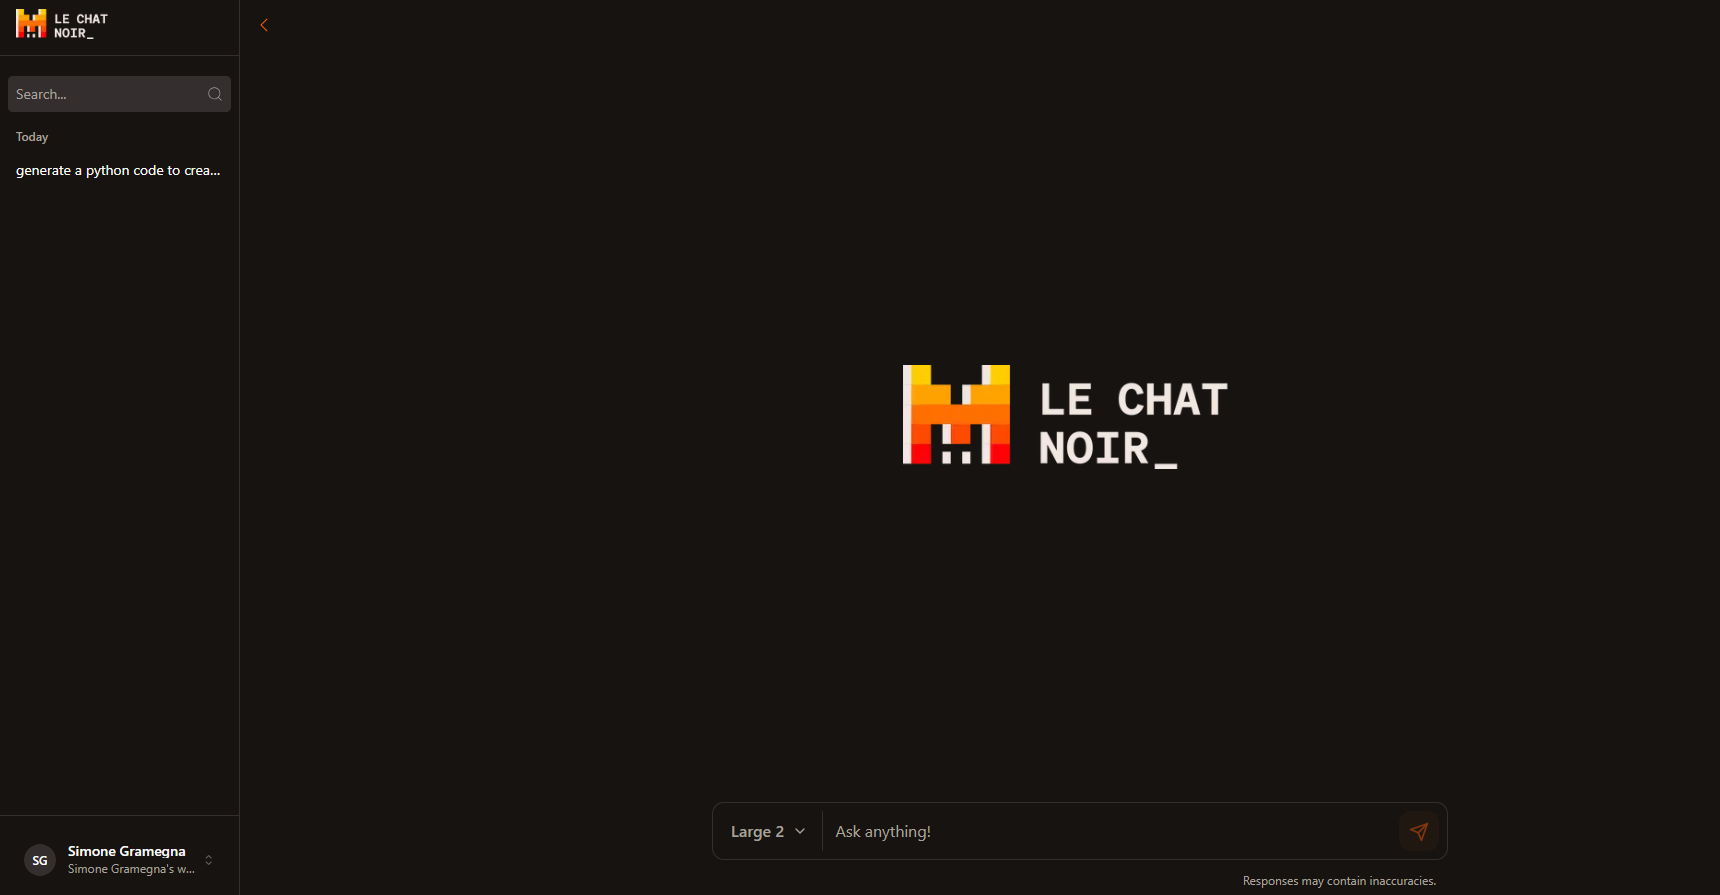
\includegraphics[width=0.9\linewidth]{Figures/fig_20.png}
    \caption{Mistral web interface}
    \label{fig_20}
\end{figure}

\subsection{State-of-the-art Multimodal Large Language Models}
An evolution of LLMs is represented by Multimodal Large Language Models MLLMs, which are capable of processing information in various forms: text, images, audio, video, and documents.
They are based on a modified version of the transformer architecture that is able to learn embeddings (vector representations) also of images, audio, and video. 
Processing these embeddings through a multi-layered network generates outputs as text and/or media \cite{wadekar2024evolution} as represented in Fig.~\ref{fig:21}.
\begin{figure}[H]
    \centering
    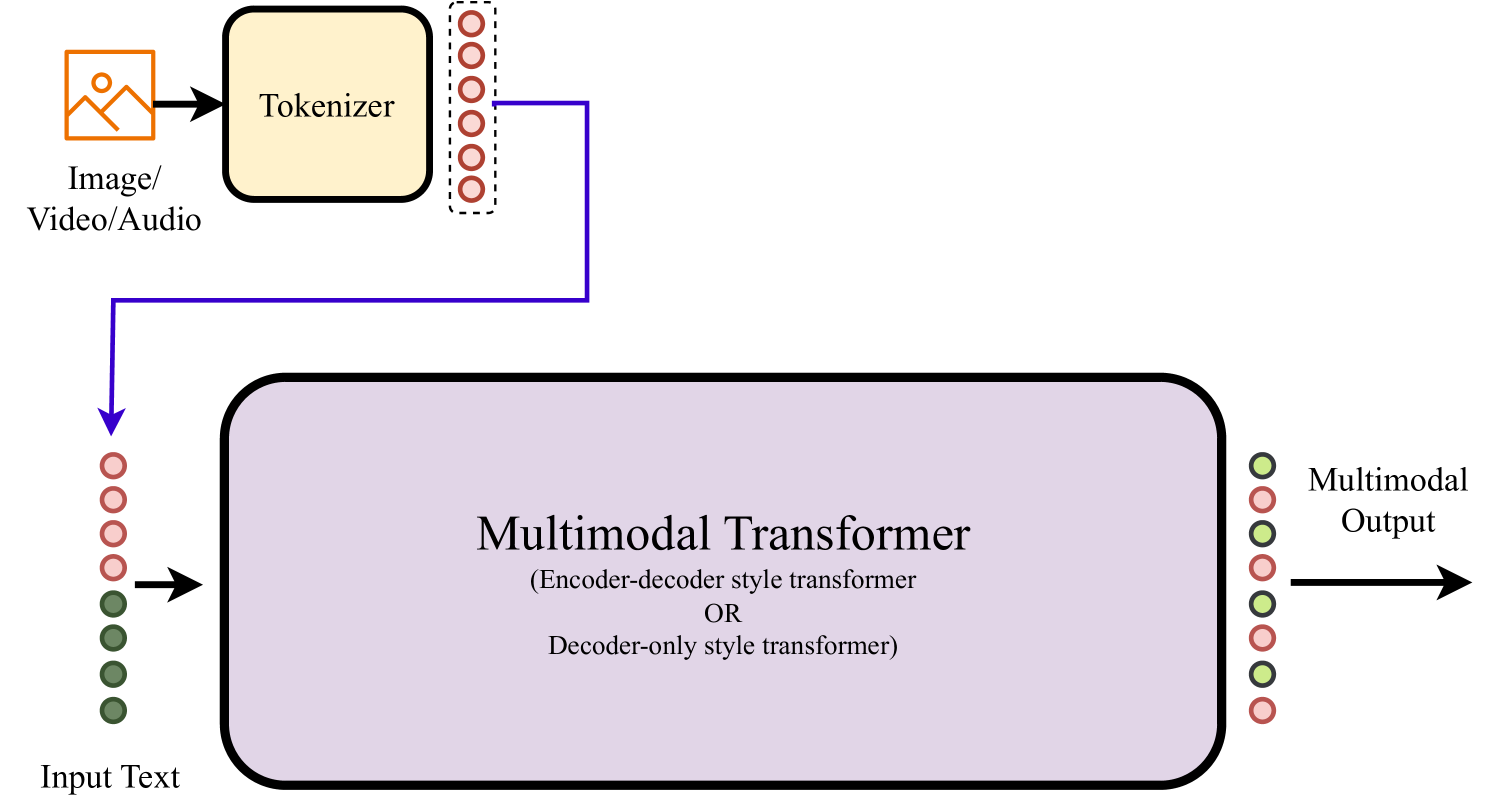
\includegraphics[width=0.9\linewidth]{Figures/fig_21.png}
    \caption{Example of multimodal transformer architecture}
    \label{fig:21}
\end{figure}

Several MLLMs have been introduced as evolutions of classic LLMs.
We will cover the following state-of-the-art MLLMs:
\begin{itemize}
    \item GPT-4
    \item Google Gemini 
    \item GLaMM
\end{itemize}

GPT-4 is the latest version of the most popular LLM: GPT.
Released in March 2023, it became available to premium users of the ChatGPT platform in three distinct versions: GPT-4, GPT-4 Turbo, and GPT-4o (omni).
These versions represent an evolution of GPT-3, enhancing performance and efficiency \cite{insights_gpt4}.
The multimodal version of GPT-4, known as GPT-4o where the "o" stands for "omni," highlighting the "omniscience" that this model is capable of:
\begin{itemize}
    \item Real-time voice communication: engage in real-time voice conversations, understanding spoken input and generating natural-sounding voice responses.
    
    \item Real-time vision: process and understand vision data like images and video and their semantics. The model can generate an image starting from text and applying styles or generating descriptions of an image.
    
    \item Data and Chart Reading: read and interpret data in forms of charts and graphs.
\end{itemize}
These features make GPT-4o a versatile and powerful tool applicable in many sectors, with particular emphasis on programming and data analysis.
Details regarding the dataset, number of parameters, and training technique are not disclosed for competitive reasons.

The latest evolution of Google's LLMs is Gemini \cite{gemini_introduction}.
It has been introduced in 2023 and is the evolution of Bard: the chatbot based on PaLM, which is discussed before.
Gemini is a proprietary model and it has proven to be superior to its rival GPT-4 on various benchmarks.

Grounding LLM (GLaMM) has been released in 2023 by Mohamed bin Zayed University of AI \cite{rasheed2024glamm}.
GLaMM is a MLLM that integrates natural language with object segmentation masks in images, combining scene-level, region-level, and pixel-level understanding.
The model uses an auto-encoder to process images and an LLM to understand natural language.
It is an open-source LLM: the source code and parameters are available on the official GitHub repository \footnote{https://github.com/mbzuai-oryx/groundingLMM}.

\section{Prompting}
\label{section:2_4_prompt_engineering}

\subsection{Definition and Structure}
At the core of interaction with LLMs are prompts, i.e., instructions written in natural language given as input to LLMs to generate responses \cite{llm_prompt}.
We can see a prompt like a mathematical function that takes in input a text and gives an output $f(x) = y$ in which $f$ is the template applied to the text of the problem.
For example, if we want to translate a phrase in English:
\begin{lstlisting}
Translate {X} in english
\end{lstlisting}
This is just a simple technique in which there is the manual creation of the template, but in literature there are more complex techniques that we are going to discuss.
In more detail, there are four main components of a prompt:
\begin{itemize}
    \item Instruction: (mandatory) a specific task or instruction you want the model to perform.
    \item Context: (optional) external information or additional context that can steer the model to better responses.
    \item Input data: (mandatory) the input or question that we are interested to find a response for.
    \item Output Indicator: (optional) the type or format of the output.
\end{itemize}

An example of output with all four components is the following:
\begin{lstlisting}
Solve the following linear equation for x and show the steps clearly. 
This is a basic algebra problem where you need to isolate x on one side of the equation.
Solve for x: 3x + 7 = 16
Provide the output in text format.
\end{lstlisting}
In this prompt the instruction is: "Solve the given linear equation for x.", the context is: "This is a basic algebra problem where you need to isolate x on one side of the equation.", the input data is: "Solve for x: 3x + 7 = 16" and the output indicator is: "Provide the output in text format."
Context and output indicator are optional components but they are useful to improve the quality of the output.

\subsection{Prompt Engineering}
Prompt Engineering is a novel discipline concerned with prompt writing and verification.
The first and simplest technique is the Zero-shot prompting in which no example is provided, and the LLM has no prior knowledge of the context, generating the output based solely on the given input prompt.
An example is the following: 
\begin{lstlisting}
Classify the text into neutral, negative or positive. 
Text: I think the vacation is okay.
Sentiment:   
\end{lstlisting}
In Few-shot prompting, on the other hand, the input prompt provided to the LLM includes a few examples. Examples are useful to achieve a better understanding of the context, this is not possible with zero-shot prompting, as we can see in the following example:
\begin{lstlisting}
Task: Translate the following sentences from italian to english.

Example "Oggi il tempo e' bello" output: "The weather is nice today"

input: "Mi piace leggere libri" // output: I love reading books
\end{lstlisting}

In Chain-of-Thought (CoT) Prompting, problem-solving is carried out step by step, breaking down a task into multiple stages to achieve more structured and accurate responses.
An example is the following:
\begin{lstlisting}
Q: Roger has 5 tennis balls. He buys 2 more cans of tennis balls. Each can has 3 tennis balls. How many tennis balls does he have now? 
A: Roger started with 5 balls. 2 cans of 3 tennis balls each is 6 tennis balls. 5 + 6 = 11. The answer is 11.  
Q: The cafeteria had 23 apples. If they used 20 to make lunch and bought 6 more, how many apples do they have?

Model output: The cafeteria had 23 apples originally. They used 20 to make lunch. So they had 23 -  20 = 3.  They bought 6 more apples, so they have 3 + 6 = 9. The answer is 9.   
\end{lstlisting}
The main issue with this technique is the manual intervention required, as the user must manually provide the reasoning that the LLM will follow.
To address this problem, a variant called Automatic Chain-of-Thought (Auto-CoT) Prompting was introduced.
Instead of manually providing the reasoning chain, the prompt includes the simple phrase, ``Let's think step-by-step`` 
for eliciting the model to engage in a CoT without adding examples of step-by-step problem solving in the prompt.
Both CoT and Auto-CoT follow a single reasoning path, but we can generate multiple reasoning paths and choose the best answer; this is the basis of the Self-consistency prompting \cite{wang2022self}.
Techniques involving multiple prompts are useful in order to decide the best reasoning strategy but we can also decide not to use any complex reasoning, but a more simple strategy that can involve the ensembling, the augmentation, the composition or the decomposition of a single prompt \cite{liu2023pre}.
In prompt ensembling, different prompts are combined on the same input in order to get a response. For instance:
\begin{lstlisting}
PR1: China's capital is [X]
PR2: [X] is capital of China
PR3: The capital of China is [X]
\end{lstlisting}

To choose the response, we can apply several strategies, including majority voting and weighted voting.
In prompt composition there is a composition of two or more subprompts in order to get the final prompt.
In contrast, in prompt decomposition one main prompt is decomposed in two or more smaller subprompts.
In LLMs, there is a significant issue that leads to incorrect responses, known as the problem of hallucinations.
We refer to hallucination, in the context of LLMs, when there is the generation of texts or responses that are grammatically and syntactically correct but deviate from the given inputs or do not align with factual accuracy \cite{ye2023cognitive}.
Prompt engineering techniques can help reduce this phenomenon, the main technique is Retrieval Augmented Generation (RAG).
In this approach, starting from an input, a knowledge base of sources (web pages, articles, etc.) is created, and the text from these sources is incorporated into the subsequent input, providing context and generating more accurate and reliable responses.
The improvement in performance and accuracy of the responses obtained from the LLM can also be achieved by incorporating the user's emotions into the prompt, known as Emotion Prompting.
Incorporating emotions can be useful in tasks such as sentiment analysis of a sentence, but this is not the case for code generation, for which various prompt engineering techniques have been introduced.
An evolution of the previously described Chain-of-Thoughts is Program of Thoughts (PoT) Prompting \cite{chen2022program}, where the large language model is given a prompt containing intermediate steps that include mathematical expressions or source code, as we can see in the following figure:
\begin{figure}[H]
    \centering
    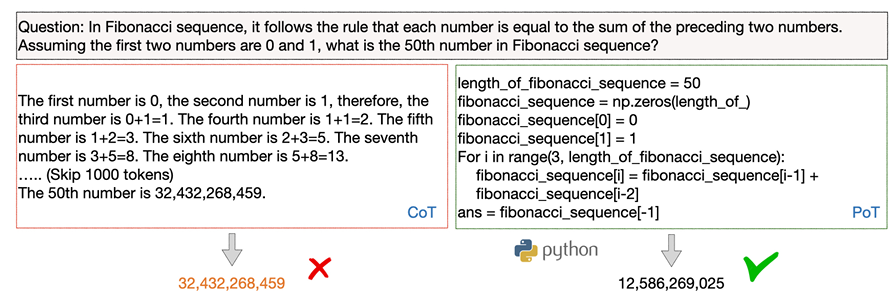
\includegraphics[width=0.7\linewidth]{Figures/fig_8.png}
    \caption{Program of Thoughts (PoT) Prompting}
    \label{fig:enter-label}
\end{figure}
Another approach is the Scratchpad Prompting in which an arbitrary sequence of intermediate tokens is generated before the final answer is provided. 
The sequence is given in a tag called "scratch" \cite{scratch,nye2021show} in which the user writes intermediate steps useful to the LLM as shown below, were it is requested to solve a simple mathematical problem:
The problem is: A store sells apples for 3 euros each. If I buy 5 apples and get a 10\% discount, how much do I pay in total?
\begin{lstlisting}
<scratch>
Perform the following calculations step by step. Write your notes in the format "Scratchpad:" for each step.

Problem: A store sells apples for 3 euros each. If I buy 5 apples and get a 10% discount, how much do I pay in total?

Scratchpad:
1. The unit price of an apple is 3 euros.
2. The number of apples purchased is 5.
3. The total cost without discount is: 3 * 5 = 15 euros.
4. The 10% discount is: 15 * 0.10 = 1.5 euros.
5. The final price after the discount is: 15 - 1.5 = 13.5 euros.
Final result: 13.5 euros.
</scratch>
\end{lstlisting}
In the example above, we begin the sequence with $<scratch>$ and we define the different steps that the model has to follow in order to solve the problem. The sequence ends with $</scratch>$.
The Rephrase and Respond (RaR) Prompting\cite{deng2023rephrase} technique automatically allows for the correction and improvement of the LLM's response through the prompt:
\begin{lstlisting}
"{question}" Rephrase and expand the question, and respond.
\end{lstlisting}
This approach has four main advantages:
\begin{enumerate}
    \item It lets the LLM self-improve the prompts while maintaining the context of the original query.

    \item It allows better aligning the human’s intended query with LLM’s preferred style of question.

    \item It expands the LLM’s thought process and adding a step that will not naturally appear when using CoT.

    \item It provides an approach for humans to interpret how LLMs understand the questions.
\end{enumerate}

Another technique to obtain more accurate and comprehensive responses is the Take a Step Back Prompting\cite{zheng2023take}, which consists of two steps. The first step involves inputting a specific question, and subsequently (step-back) inputting a more abstract, high-level question related to the task, as shown in the following figure:
\begin{figure}[H]
    \centering
    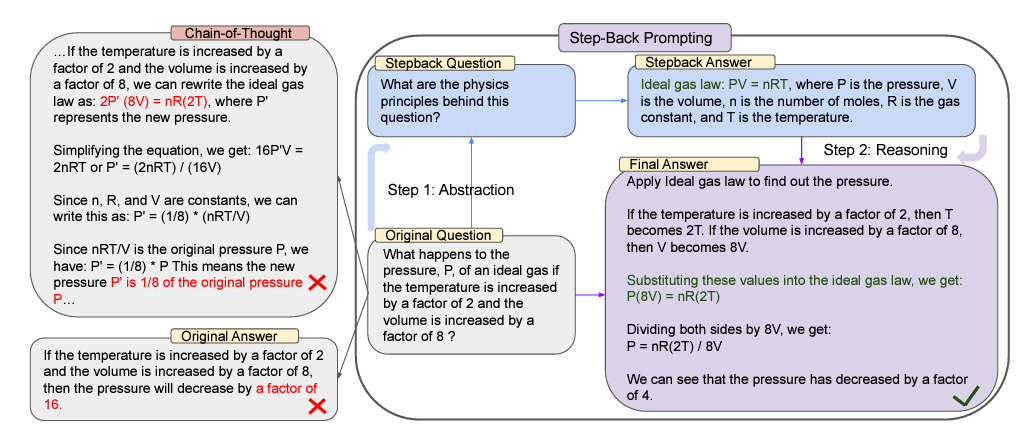
\includegraphics[width=0.9\linewidth]{Figures/fig_9.png}
    \caption{Take a Step Back Prompting}
    \label{fig:9}
\end{figure}

\subsection{Prompt engineering in Multimodal Large Language Models}
State-of-the-art prompt engineering techniques aim, when given as input to a LLM, to generate text.
MLLMs allow for incorporating media such as image into prompts.
Main tasks involving MLLMs are:
\begin{itemize}
    \item Image generation
    \item Image classification
    \item Image editing
\end{itemize}

A preliminary approach to image classification is the use of zero-shot prompting and few-shot prompting \cite{chen2023unleashing}.
In zero-shot prompting for image generation, no input examples are provided, but only the instruction to be executed, for example:
\begin{lstlisting}
Classify the follwing image: [image.png]
\end{lstlisting}
In few-shot prompting, examples are provided to the model, for instance:
\begin{lstlisting}
Given: [image1.png], [image2.png], [image3.png], classify the following image: [image.png]
\end{lstlisting}
Zero-shot prompting and few-shot prompting can be also used in image generation.
However, this task is more complex and it can benefit from user feedback.
An example is drawing a stick figure using letters of the alphabet \cite{proptingguide_image}, where the process starts from an initial prompt, such as:
\begin{lstlisting}
Produce TikZ code that draws a person composed from letters in the alphabet. The arms and torso can be the letter Y, the face can be the letter O (add some facial features) and the legs can be the legs of the letter H. Feel free to add other features.    
\end{lstlisting}
The generated image is refined by adding details: 
\begin{lstlisting}
- The torso is a bit too long, the arms are too short 
  and it looks like the right arm is carrying the face instead of the face being right above the torso. Could you correct this please? 

- Please add a shirt and pants.
\end{lstlisting}
As we can see in the following example, where the latest version of ChatGPT, GPT4, has been applied:
\begin{figure}[H]
    \centering
    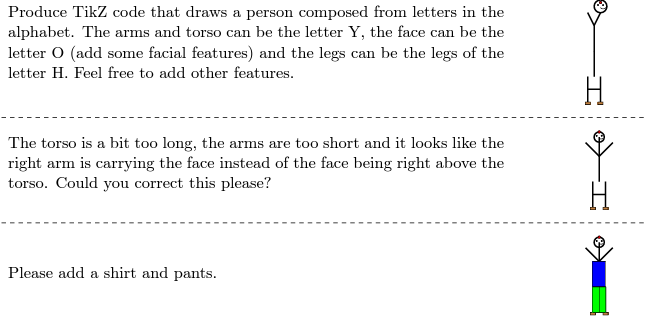
\includegraphics[width=0.8\linewidth]{Figures/fig_10.png}
    \caption{Drawing using GPT4}
    \label{fig:10}
\end{figure}
In image generation the characteristics of an image can be specified not only using user feedback but also using style modifiers.
They are descriptors that consistently produce certain styles, for example: "tinted red", "made of glass", and combining those together they produce a more specific style \cite{lp_style}.
For example, we want to generate, using DALL-E, a picture of a pyramid.
The first picture is generated without using any modifier:
\begin{figure}[H]
    \centering
    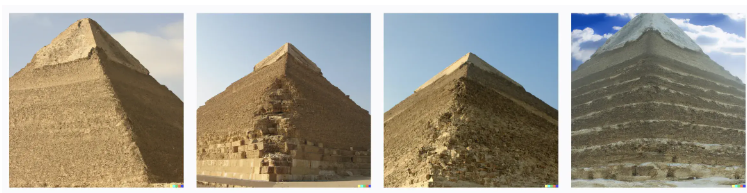
\includegraphics[width=0.9\linewidth]{Figures/fig_11.png}
    \caption{Pyramid picture with no modifiers}
    \label{fig:11}
\end{figure}
The second picture is generated using the prompt with three modifiers: A pyramid made of glass, rendered in Unity and tinted red getting the following result:
\begin{figure}[H]
    \centering
    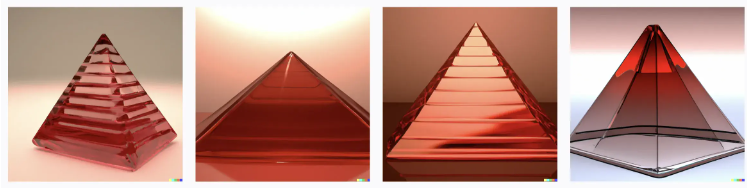
\includegraphics[width=0.9\linewidth]{Figures/fig_12.png}
    \caption{Pyramid picture with modifiers}
    \label{fig:12}
\end{figure}
In the prompt, in order to improve quality, we can add generic adjectives like: "amazing", "good", "beautiful" that are called quality boosters \cite{oppenlaender2023taxonomy}.
The Latin motto "repetita iuvant" that means that repeating words is useful can be applied in a certain sense in a prompt for image generation, the repetition technique gives more importance to some adjective instead of another it is possible to repeat more times the word, giving emphasis to it.
For example, the generation of an image of a waterfall, but we want to emphasise the beauty of the picture we can use this following prompt:
\begin{lstlisting}
A very very very very very beautiful painting of a mountain next to a waterfall
\end{lstlisting}
In this case the word "very" is repeated five times in order to give more importance to the adjective beautiful.
Since repeating terms in a prompt can be weird and inaccurate, it is possible to use weighted terms technique\cite{weighted_terms}. In this technique a term has a numerical value (positive or negative) that corresponds to the weight, i.e., the importance of that term.
For example, the generation of a picture of a mountain without trees, we use this prompt:
\begin{lstlisting}
mountain | tree:-10.
\end{lstlisting}
in which the tree has negative weight and it doesn't have importance getting this result, as we can see in the figure \ref{fig:15}:
\begin{figure}[H]
    \centering
    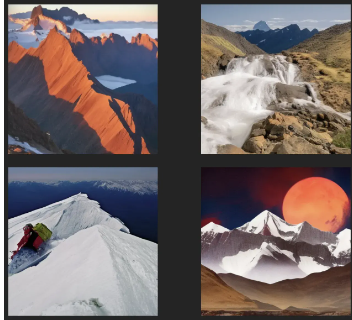
\includegraphics[width=0.5\linewidth]{Figures/fig_15.png}
    \caption{Weighted terms image}
    \label{fig:15}
\end{figure}

Another approach in image generation is negative prompting, those allow users to exclude unwanted features and enhance the quality output.
Negative prompts are complementary to  positive prompts which describe what the user wants, including the main subject and how it should look \cite{medium_negative}.
For example, we want to generate using a diffusion model a portrait of a man without moustache, so the prompt is:
\begin{lstlisting}
- Positive prompt: Portrait photo of a man.
- Negative prompt: Moustache
\end{lstlisting}
Negative prompts can be applied on any image feature like: colors, lighting problems, unwanted elements, image quality and style.
The Multimodal Chain-of-Thought prompting technique \cite{zhang2023multimodal} is a variation of the Chain-of-Thought technique (CoT).
This technique in Multi-CoT is enhanced by incorporating in the prompt text and visual inputs.
The technique consists in two stages:
\begin{enumerate}
    \item Rationale generation: the model processes the multimodal inputs in order to generate an intermediate reasoning chain (rationale). The rationale explains the logical steps required to arrive at the final answer, using both textual and visual content as context.

    \item Answer inference: the generated rationale is combined with the original input and used by the model to infer the final answer.
\end{enumerate}
as we can see in the figure \ref{fig:16} below:
\begin{figure}[H]
    \centering
    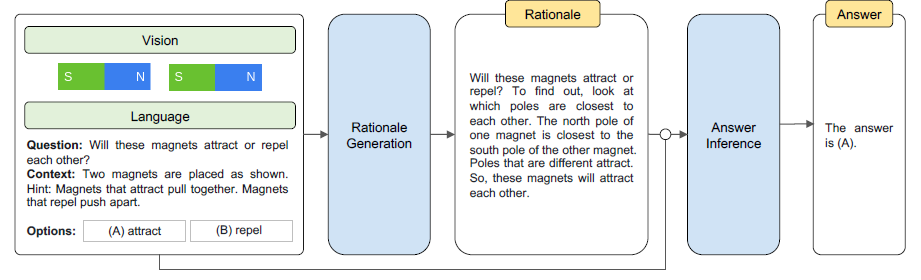
\includegraphics[width=0.9\linewidth]{Figures/fig_16.png}
    \caption{Multimodal Chain-of-Thought}
    \label{fig:16}
\end{figure}
Similar to the multimodal chain-of-thought, the Chain of Images (CoI) prompting technique \cite{meng2023chain} generates a series of images as intermediate representations in order to solve problems starting from a textual prompt.
 


\chapter{The Prompt Engineering Ontology: Requirements Specification}
\label{chapter:3_design}
This chapter details the design phase of the Prompt Engineering Ontology PEO, based on LOT, a state-of-the-art ontology engineering methodology.
Compared to other methodologies analysed, LOT is a recent methodology, introduced in 2022, and has been used in various projects such as the 'Ciudades Abiertas' project \cite{ciudad} for the construction of a set of ontologies used for sharing open data, and the BIMERR project \cite{bimerr}, in which ontologies for sustainable construction were developed \cite{bountouni2021bimerr}, among many others available on the LOT methodology website \footnote{https://lot.linkeddata.es/}.
LOT has not only been successfully applied in industrial projects, but also in the development of various research ontologies, as seen in Chapter~\ref{chapter:background}, as it provides a straightforward and iterative method for designing and developing ontologies.
Another reason for choosing LOT is its ease of learning, as it is inspired by the agile methodology in software development. The Linked Open Terms project not only provides very useful examples of ontologies to draw inspiration. LOT offers a Github repository \cite{lot_github} with all the necessary resources to be used in the specification of requirements.
This last aspect is very important because the main drawback of the other methodologies analysed is the lack of concrete guidelines and the relevant tools to use, tools that, when mentioned, are often obsolete or inaccessible.
This complicates the work of a developer who is approaching ontology engineering for the first time, as he needs to understand the fundamentals of the methodology but also figures out which development, validation, and testing software to use.
The LOT methodology, thanks not only to the numerous available resources but also to the clear and precise description of the method and the recent tools to be used, resolves these issues and simplifies the developer's work.
The LOT methodology has an inherently iterative nature and is oriented towards the publication of ontologies according to the FAIR principles \cite{fair_eu}, including specific recommendations, tips and potential
tools that can be helpful to ontology developers.
Moreover, the methodology extends the state-of-art methodologies like NeOn and Methontology with a modern approach.

The LOT methodology was preferred over recently introduced techniques that involve the use of LLMs.
Although these techniques automate the process, they are computationally expensive and require numerous checks to verify the syntactic and semantic correctness of the produced artifact.
Another downside is the lack of actual ontology projects implemented using LLMs, as these are very recent techniques that have not been tested on real projects but only on experimental cases.
In the following sections, the application of the LOT methodology, methodology that has been discussed in Chapter \ref{chapter:background}, to the design and implementation of PEO will be described, following the workflow outlined and described in the background chapter.
\section{Use Case Specification}
The LOT methodology includes six mandatory phases (plus one optional) in the ontology requirements specification.
At the end of each phase, a document is produced containing the analysed aspect of the specifications, as shown in the following figure \ref{fig:13}:
\begin{figure}[H]
    \centering
    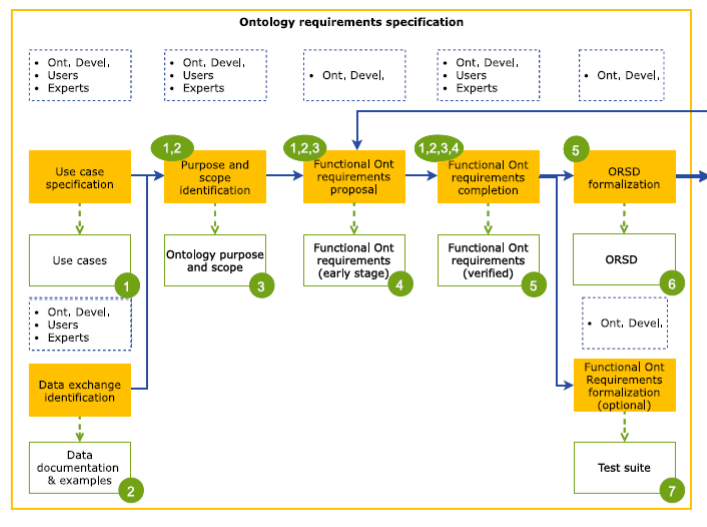
\includegraphics[width=0.9\linewidth]{Figures/fig_13.PNG}
    \caption{Ontology requirements specification workflow}
    \label{fig:13}
\end{figure}
In detail the phases are the following:
\begin{enumerate}
    \item Use case specification
    \item Data exchange identification
    \item Purpose and scope identification
    \item Functional ontology requirements proposal
    \item Functional ontology requirements completion
    \item ORSD formalization 
    \item Functional ontology requirements formalization (optional)
\end{enumerate}
The first step in the design of PEO is the use case specification, this phase involves domain experts, ontology developers and users and it has the goal to imagine and specify how the ontology can be used in real life by real users.
Taking into account the domain, the possible use and the possible users we decided to specify ten use cases.
Each use case has a name, a description, a list of actors and a flow.
\paragraph{Use case 1}
\begin{itemize}
    \item Name: Optimizing LLM Responses
    \item Description: Researchers use PEO to design optimized prompts that improve LLM response quality.
    \item Actors: Researcher, PEO, LLM.
    \item Flow: The researcher uses the ontology to identify appropriate prompts for different types of tasks creating a set of selected prompts. Selected prompts are given as input to the LLM and responses are evaluated according to specific metrics on consistency, completeness and quality decided by the researcher.
\end{itemize}
\paragraph{Use case 2}
\begin{itemize}
    \item Name: Bias analysis
    \item Description: Researchers use PEO to generate responses and detect bias in the considered LLMs.
    \item Actors: Researcher, PEO, LLMs
    \item Flow: The researcher uses the ontology to generate prompts on sensitive topics (e.g., gender, ethnicity) and prompts are tested on one or more LLMs. Responses are collected using bias and fairness metrics and results are collected in order to improve prompts and considered models. 
\end{itemize}

\paragraph{Use case 3}
\begin{itemize}
    \item Name: Code generation
    \item Description: Developers use prompt engineering techniques applied to a chosen LLM to generate source code in a specific programming language for a specific task.
    \item Actors: Developers, PEO, LLM
    \item Flow: The developer is working on an Android application written in Java and needs code to control the actions on a button. Using the ontology, he chooses the most appropriate prompt engineering technique and applies it to the creation of the prompt to a large language model of his choice,  resulting in Java code as output. The code is tested and integrated into the application. 
\end{itemize}

\paragraph{Use case 4}
\begin{itemize}
    \item Name: Prompt engineering lesson
    \item Description: The teacher uses PEO to teach prompt engineering techniques exploring different techniques and prompt described.
    \item Actors: Teacher, students, PEO. 
    \item Flow: The teacher opens the ontology and shows with proper explanation different prompt engineering techniques represented in the ontology.
\end{itemize}

\paragraph{Use case 5}
\begin{itemize}
    \item Name: LLMs lesson
    \item Description: The teacher uses PEO to teach the different LLMs available.
    \item Actors: Teacher, students, PEO.
    \item Flow: The teacher opens the ontology and shows with proper explanation different LLMs represented in the ontology. 
\end{itemize}
\paragraph{Use case 6}
\begin{itemize}
    \item Name: Social media content creation
    \item Description: The content creator uses PEO to generate prompts that optimize the creation of articles, social media posts and other textual content.
    \item Actors:  Content creator, PEO, LLM
    \item Flow: The content creator opens the ontology and chooses the appropriate technique in order to generate text for a post on social media using a specific large language model. The content creator adapts the response according to his target.
\end{itemize}

\paragraph{Use case 7}
\begin{itemize}
    \item Name: Image generation
    \item Description: The content creator uses PEO to create a prompt to be given as input to a specific large language model capable of generating an image.
    \item Actors: Content creator, PEO, LLM.
    \item Flow: The content creator wants to create an AI-generated image for a video and he uses the ontology to choose the best large language models able to generate image, he chooses the prompt engineering technique to create the prompt in order to generate image. He watches the output and he continues to use the ontology to generate prompts in order to refine the image.
\end{itemize}

\paragraph{Use case 8}
\begin{itemize}
    \item Name: Prompt engineering experiments
    \item Description: Students use PEO to explore and create effective prompts to improve language model responses.
    \item Actors: Students, PEO, LLM.
    \item Flow: Students explore the ontology in order to understand different prompting techniques applying them to a chosen large language model.
\end{itemize}

\paragraph{Use case 9}
\begin{itemize}
    \item Name: Large language models learning
    \item Description: Students use PEO to learn different types of large language models.
    \item Actors: Students, PEO
    \item Flow: Students explore different large language models represented in the ontology and the relations among them, learning all the features of each large language model.
\end{itemize}

\paragraph{Use case 10}
\begin{itemize}
    \item Name: Explanation computer science topics
    \item Description: Student wants to generate a prompt using PEO in order to explain a computer science topic.
    \item Actors: Student, PEO, LLM
    \item Flow: The student uses the ontology to choose the most appropriate prompt engineering technique in order to generate using large language models. The student reads the obtained LLM response and can create a new prompt using another technique represented in the ontology.
\end{itemize}

\section{Data Exchange Identification}
The goal of the data exchange identification activity is to provide the necessary documentation about the domain to be modelled.
Essentially, this phase involves gathering heterogeneous sources of information, such as scientific papers, websites, datasets, and similar existing ontologies.
Since LOT does not provide a clear indication on how to represent this documentation, we simply noted the URLs of the gathered resources.
The following list of papers was chosen as a source for PEO:

\begin{itemize}
\item A Systematic Survey of Prompt Engineering in Large Language Models: Techniques and Applications \cite{sahoo2024systematic}

\item Pre-train, Prompt, and Predict: A Systematic Survey of Prompting Methods in Natural Language Processing \cite{liu2023pre}

\item A Survey of Large Language Models \cite{zhao2023survey}

\item Investigating Prompt Engineering in Diffusion
Models \cite{witteveen2022investigating}

\item A Survey on Large Language Models: Applications,
Challenges, Limitations, and Practical Usage \cite{hadi2023survey}

\item Large Language Models: A Survey \cite{minaee2024large}
\end{itemize}
The list of website chosen is the following:
\begin{itemize}
    \item \href{https://www.promptingguide.ai/}{Prompting Guide}
    
    \item \href{https://github.com/Hannibal046/Awesome-LLM}{Awesome-LLM}

    \item \href{https://llmmodels.org/}{List of LLMs}

    \item \href{https://learnprompting.org/}{Learn prompting}
\end{itemize}
We decided to select these research papers and websites to build a well-structured and comprehensive ontology for prompt engineering and large language models. The academic papers provide in-depth analyses of prompting techniques, their applications, and the evolution of LLMs, offering a strong theoretical foundation. Meanwhile, the chosen websites serve as practical resources, curating up-to-date information on LLM architectures, prompting strategies and real-world use cases. 


\section{Purpose and Scope Identification}
From use cases and the domain documentation provided in the data exchange identification task, in this phase there is the specification of the purpose: what is the objective of PEO and the specification of the scope of the ontology: what it is going to be represented in the ontology.
The objective of PEO is to formalize knowledge about the creation and various types of prompts for the different LLMs available by making it accessible to both experienced and less experienced users.
PEO aims at covering the following scope:
\begin{itemize}
    \item LLMs available to users
    \item Prompt engineering techniques
    \item Task that can be solved using a LLM
    \item Examples of prompts specific to the LLM
\end{itemize}
In general, the goal of the project and the ontology is to create a resource accessible to everyone on a recently introduced topic, for which there are not many available resources.
This resource aims to support not only the learning but also the application of prompt engineering techniques and LLMs.

\section{Functional Ontology Requirements Specification}
In LOT methodology there are three possible ways to specify the requirements: CQs, natural language statements and tabular information containing concepts, relations, and attributes.
As seen in Chapter~\ref{chapter:2_background}, competency questions are widely used in ontology engineering and allow for clearly expressing the functional requirements of an ontology.
In the case of PEO, based on the use cases and the purpose and scope identification described earlier, we have identified sixteen CQs:
\begin{itemize}
    \item CQ1: What is prompt engineering?

    \item CQ2: What is a prompt?

    \item CQ3: What are prompting techniques?

    \item CQ4: What are image prompting techniques?

    \item CQ5: What are code prompting techniques?

    \item CQ6: Which task does a prompt solve?

    \item CQ7: Which prompts are generated using a prompting technique?

    \item CQ8: What are the responses that follow each prompt?

    \item CQ9: What are possible tasks?

    \item CQ10: Which tasks are related to the text?

    \item CQ11: What is a chat?

    \item CQ12: What is a large language model?

    \item CQ13: What types of large language models are available?

    \item CQ14: What are large language models architectures?

    \item CQ15: What are large language models capabilities?

    \item CQ16: What companies develop large language models?
\end{itemize}

CQs are saved into an excel file, the template is available in the official Github repository \footnote{https://github.com/oeg-upm/LOT-resources}.
The Excel file not only contains the CQs, but also specifies for each one: the identifier, the domain, the answer, the status (Proposed, Accepted, Rejected, Pending, Deprecated), comments, and priority (high, medium, and low).
All the CQs have a high priority, as they form the foundation of PEO, covering both prompt engineering and LLMs.

\section{Document Formalization}
The final step in the specification of ontology requirements is the writing of the ORSD, a document that gathers the main information defined in the previous phase, namely the purpose and scope of the ontology, the use cases, the functional requirements (expressed through CQs), and the non-functional requirements.
First introduced by the NeOn methodology, which we discussed in the previous chapter, the writing of the ORSD follows a specific sequence of tasks to ensure its correctness and completeness.
The workflow \cite{suarez2009write} involves a sequence of eight tasks, starting from ontological needs: 
\begin{enumerate}
    \item Identify purpose, scope and implementation language.
    \item Identify intended end-users
    \item Identify intended uses
    \item Identify requirements
    \item Group requirements
    \item Validate the set of requirements
    \item Prioritize requirements
    \item Extract terminology and its frequency
\end{enumerate}
LOT adopts (a customized version of) the ORSD introduced by NeOn.
Unlike NeOn, it does not consider the "user" field as mandatory, and the glossary of terms is built starting from the competency questions.
In writing the ORSD for PEO, the  template from the official LOT repository \footnote{https://github.com/oeg-upm/LOT-resources/tree/master/templates\%20for\%20ORSD} was used. 
In the document, the information obtained in the previous phases has been included, namely purpose and scope identification and ontology requirements in the form of CQs.
Additionally, further information that emerged during the requirements gathering phase has also been included:
\begin{itemize}
    \item Implementation language 
    \item Intended End-Users 
    \item Intended Uses
    \item Non-Functional Requirements
\end{itemize}
In detail, the implementation language is OWL using the Protegé software\cite{protege_sw}, an open-source popular software released by Stanford University.
As seen in the use cases, the intended end-users of PEO are:
\begin{itemize}
    \item Researchers in the field of AI using LLMs for research purpose.
    \item Software engineers and developers.
    \item Educators and trainers teaching students or professionals about AI and prompt engineering, using the ontology as a learning and instructional tool.
    \item Content Creators using LLMs for generating content.
    \item Undergraduate and high school students learning about AI, LLMs and prompt engineering, using the ontology to understand core concepts and experiment with language models.
\end{itemize}
Starting from the use cases, it is possible to easily deduce the intended uses:
\begin{itemize}
    \item Prompt generation
    \item LLMs learning
    \item Prompt engineering learning
    \item Prompt generation for a specific task
\end{itemize}
Regarding non-functional requirements, i.e., the characteristics, qualities and general aspects not related to the ontology content that the ontology should satisfy, we have identified three non-functional requirements:
\begin{itemize}
    \item NFR1: The ontology must be published on main ontology repositories
    \item NFR2: The ontology must have exhaustive documentation.
    \item NFR3: The ontology must be easy to update.
\end{itemize}
Those non-functional requirements match with the desired properties of PEO, since the ontology has to be accessible for everyone by publishing on main ontology repositories. The documentation  must be exhaustive and clear for users to understand the content of the ontology and it could be useful for possible updates.






\chapter{The Prompt Engineering Ontology: Conceptualization and Encoding}
\label{chapter:4_implementation}
This chapter describes the implementation of PEO by following the approach described by the LOT methodology. 
In the section \ref{section:4_1_conceptualization} we discuss the conceptualization of PEO, in the section \ref{section:4_2_reuse} we discuss the reuse of existing design patterns and in the section \ref{section:4_3_encoding} we describe the encoding process. 
\begin{figure}[H]
    \centering
    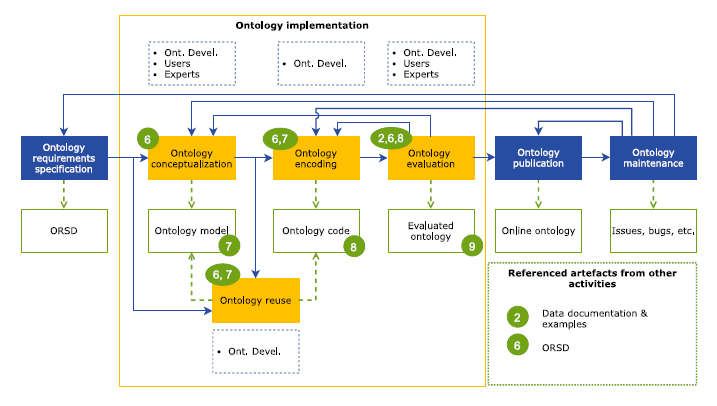
\includegraphics[width=0.9\linewidth]{Figures/fig_14.png}
    \caption{Ontology implementation workflow}
    \label{fig:14}
\end{figure}
Fig. \ref{fig:14} represents the ontology implementation workflow according to LOT.
At the end of this phase, the output is an ontology ready to be published and to be made available online.

\section{Conceptualization}
\label{section:4_1_conceptualization}
The first step in the ontology implementation is the ontology conceptualization, we define of all main concepts in the ontology with the relations among them.
We used \href{draw.io}{https://app.diagrams.net/} software: a free easy-to-use diagramming tool that allows to represent UML diagrams and many more. 
We chose this software over other diagramming tools because it is intuitive, easy to use, and frequently updated moreover with draw.io. It is possible to export diagrams in other formats like: svg, pdf and png in high resolution.
Starting from the CQs, we chose a top-down strategy in order to model the domain of prompt engineering and LLMs, modelling first major concepts and then going more into detail.
A LLM is represented using four dimensions:
\begin{enumerate}
    \item Type: type of LLM which. Each type of LLM has one or more instances representing versions of that LLM.

    \item Organization: organization that creates the LLM.

    \item Base model: the deep learning model at the base of the architecture of the LLM. This concept represents an attribute of a LLM.

    \item Capability: the capability of a LLM, it is represents an attribute of a LLM.
\end{enumerate}
These concepts provide a representation of various aspects of LLMs, from their underlying architecture to the organizations that develop them, which can range from universities and research institutions to companies with business-oriented goals.
A fundamental aspect is the representation of the capabilities of LLMs.
In fact, the ontology will not only include LLMs capable of processing text but also multimodal models capable of handling more complex data types, such as images, audio, video, and source code.\\
Regarding prompt engineering, starting from the user's perspective, we decided to model the domain using the following concepts:
\begin{itemize}
    \item Prompting technique: gathers all the prompting techniques, each prompting technique is a sub concept.

    \item Prompt: this is the base concept, a single prompt provided as input in the context of a chat with a specific LLM, followed by a response. The prompt can be generated using a prompting technique.

    \item Chat: represents the context of a prompt with a specific LLM and it can include one or more prompts and responses.

    \item Response: represents the response generated by LLM after the input of a prompt in the context of a specific chat.
\end{itemize}


In addition, there is also the modelling of the concept "Task" that represents the tasks to be solved using LLMs by applying prompting techniques.
This concept has sub concepts specific for the task that has to be solved like: image task, text task, code task, audio task and video tasks, each one of those concepts has other sub concepts, e.g., the "text task" has as sub concepts text summarization, emotion classification, text translation.

The concepts of "Chat" and "Prompt" are introduced to decouple each prompting technique from a specific LLM, ensuring their independence.
The intuition behind this conceptualization is that a prompt is created using a specific prompting technique and applied in the context of a specific chat with a version of LLM producing a response.
The connection with the concept of Task lies in solving a specific task through the use of an instance of a prompting technique.
Once defined the major concepts in the ontology, we define the relations between these concepts.
Starting from the LLM, each sub concept like GPT, Mistral, Gemini is involved in the following relations:
\begin{itemize}
    \item develops: an organization develops a LLM type, for example Google develops Gemini.

    \item has\_architecture: a LLM type has an architecture based on a specific base model. For example GPT has architecture the decoder-only model.
    
    \item has\_capability: a LLM type is connected to a specific capability.
\end{itemize}
As we have seen, the aspect of different versions of the same model must be considered and appropriately represented.
To achieve this, we have used two distinct relations:
\begin{itemize}
    \item has\_variant: this relation represents a contemporaneity between two models, where a model $x$ is a variant of a model $y$, and this does not represent an evolution of model $x$. For example Mistral-7B has variant Codestral (a version of Mistral specific for source code processing.)

    \item evolves: unlike has variant, this relation represents a temporal succession between an older model and a newer model, for example GPT-3 evolves GPT-4, where GPT-4 is a more recent and powerful version of GPT. For this relation, we have introduced also the inverse relation evolved from.
\end{itemize}
Another specific aspect considered is the presence of relations between organizations developing LLMs, where one organization is part of another organization, for example, DeepMind is a research organization and is part of Google.
We created two relations called: has organization and is organization of in order to represent this aspect in the ontology.
\begin{figure}[H]
    \centering
    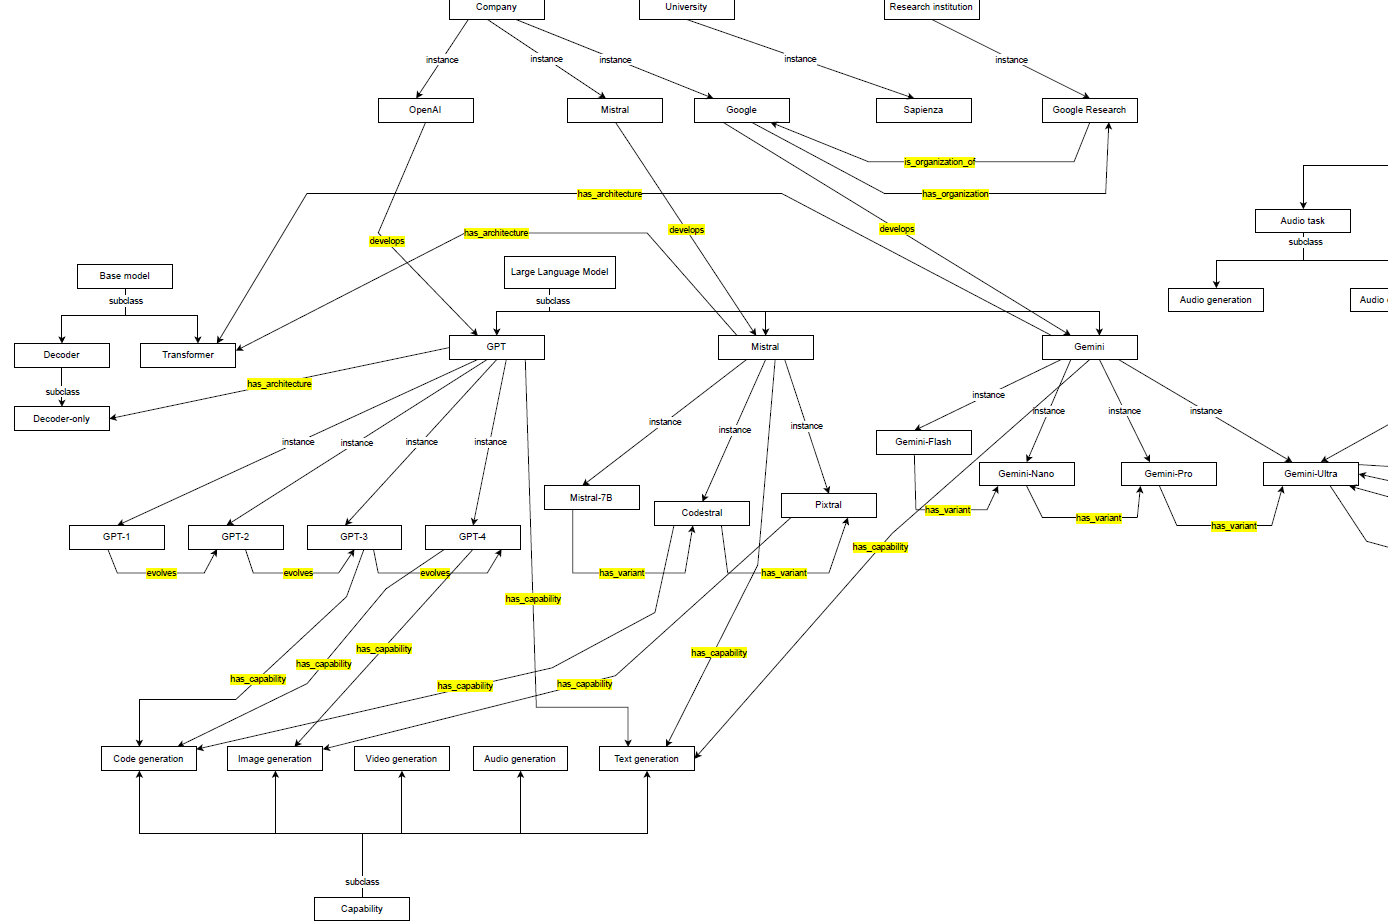
\includegraphics[width=0.9\linewidth]{Figures/fig_26.png}
    \caption{LLMs dimensions conceptualization}
    \label{fig:26}
\end{figure}
The Fig. \ref{fig:26} shows the conceptualization scheme for LLMs.

Regarding the prompt domain, the following relations have been created in order to properly connect the introduced concepts:

\begin{itemize}
    \item solves\_task: connects a prompting technique with a task. The inverse relation is: solved by.

    \item is\_used\_in\_prompt: connects a prompting technique with a prompt. The inverse relation is: prompt generated using.

    \item has\_context: connects a prompt with its context, i.e., a chat where such prompt and possibly more are connected to. The inverse relation is: has prompt.

    \item uses\_model: connects a chat with a LLM that is used to input prompts and generate responses. The inverse relation is: is used in chat.

    \item generates\_response: connects a LLM with the response generated after a prompt to such LLM. The inverse relation is: response generated using.

    \item prompt\_follows\_response: connects a prompt with its response, the inverse relation is: response followed by prompt.

    \item has\_response: connects a chat with a response, the inverse relation is: is response of.
\end{itemize}

\begin{figure}[H]
    \centering
    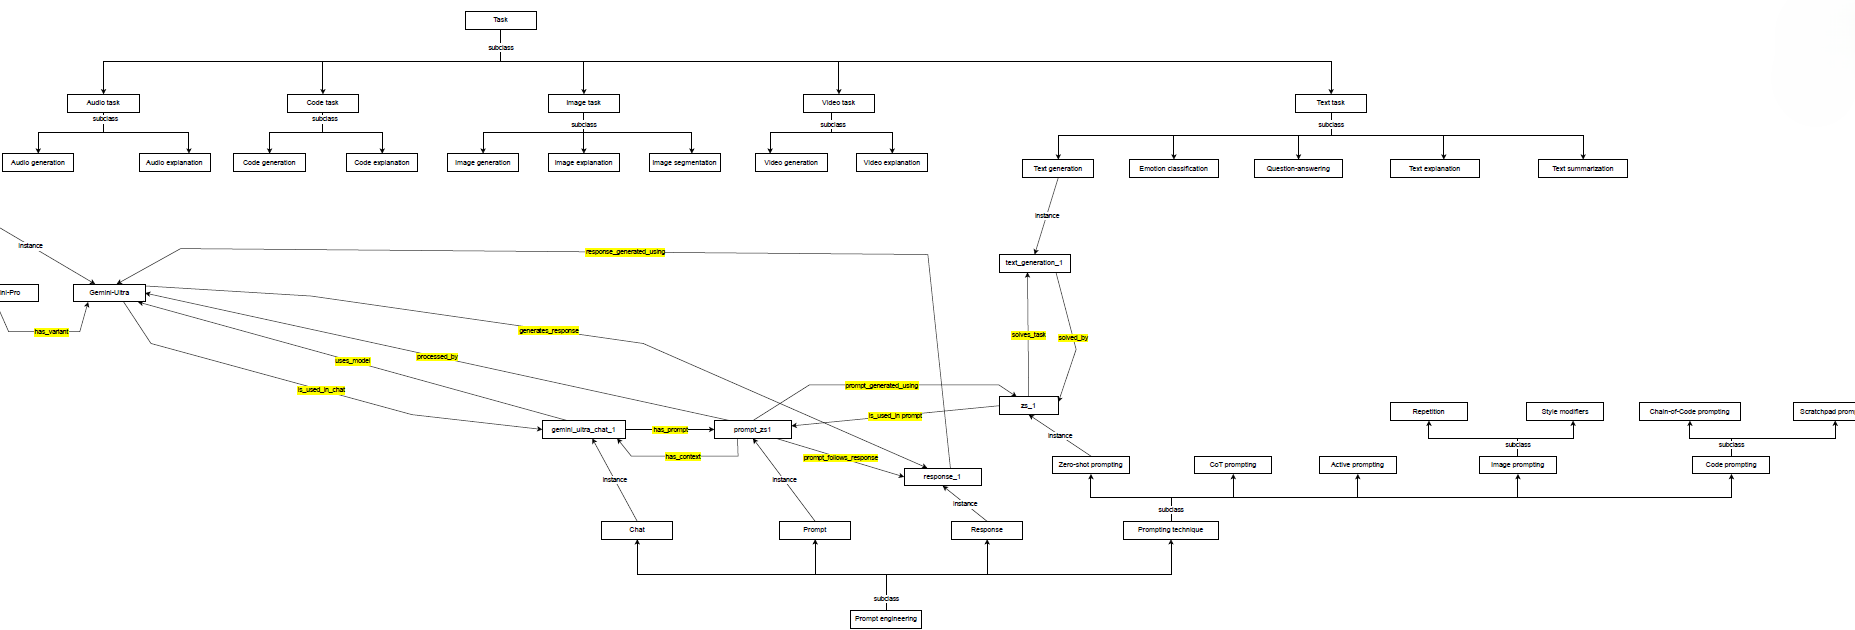
\includegraphics[width=0.9\linewidth]{Figures/fig_27.png}
    \caption{Prompt engineering\\ dimensions conceptualization}
    \label{fig:27}
\end{figure}
The Fig. \ref{fig:27} shows the conceptualization for Prompt Engineering part.

After completing the conceptualization phase, the process can proceed to ontology reuse and ontology encoding.
This involves first identifying similar ontologies within the domain of interest for potential reuse, followed by implementing and encoding the defined concepts using dedicated software tools.

\section{Reuse}
\label{section:4_2_reuse}
Before proceeding with ontology encoding, it is necessary to consider any similar ontologies that can be reused in the creation of the prompt engineering ontology. There are two types of reuse:
\begin{itemize}
    \item Hard reuse: involves directly importing an entire ontology, rigidly incorporating it. Classes and properties are used without modification, ensuring semantic consistency but creating strong dependency on the original ontology.

    \item Soft reuse: involves adapting or copying specific concepts without importing the complete ontology. This approach offers more flexibility, allowing customization, but it may introduce semantic inconsistencies or redundancies 
\end{itemize}

\subsection{Ontology Design Patterns Reuse}
\label{subsection:4_2_1_design_patterns}
During the design of PEO, we decided to use three design patterns:
\begin{itemize}
    \item Description pattern
    \item Sequence pattern
    \item Task Execution
\end{itemize}

The description pattern is used in the definition of subclasses of LLM class, where its subclasses describe the LLM class.\cite{description_pattern}
In fact, this ODP allows the designer to represent both a (descriptive) context and the elements that characterize and are involved in that context.

\begin{figure}[H]
    \centering
    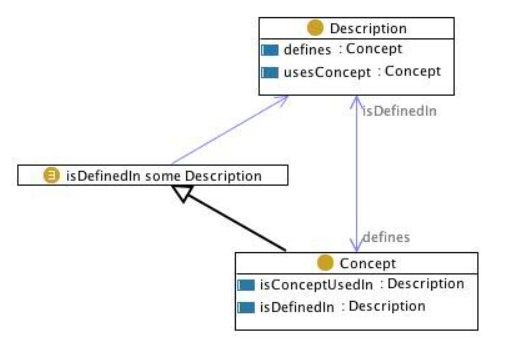
\includegraphics[width=0.6\linewidth]{Figures/fig_73.png}
    \caption{Description pattern}
    \label{fig:73}
\end{figure}
The Fig. \ref{fig:73} shows graphically the Description pattern.

The sequence pattern is used in the ontology to represent evolutionary aspects, specifically among instances of LLMs, involving the relationships evolves and evolves\_from.
This ontology design pattern allows to represent and reason over transitive or intransitive sequences of any kind \cite{sequence_pattern}.
\begin{figure}[H]
    \centering
    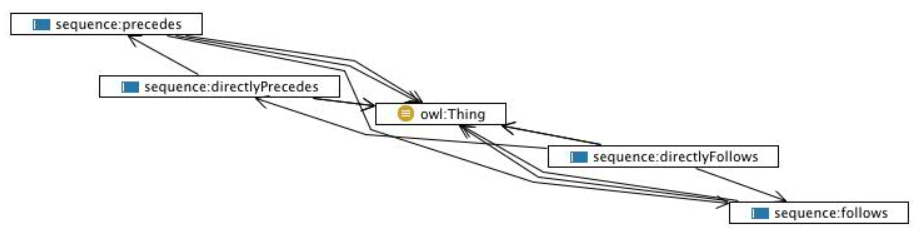
\includegraphics[width=0.8\linewidth]{Figures/fig_74.png}
    \caption{Sequence pattern}
    \label{fig:74}
\end{figure}
The Fig. \ref{fig:74} shows graphically the Sequence pattern.

The task execution pattern is partially used in the representation of task instances executed (solved) by an instance of a prompting technique. More in general, this ODP allows designers to make assertions on roles played by agents without involving the agents that play that roles, and vice versa\cite{task_execution}.

\begin{figure}[H]
    \centering
    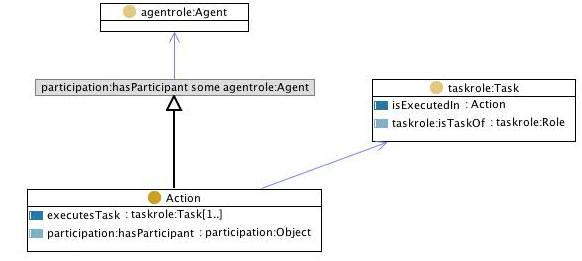
\includegraphics[width=0.8\linewidth]{Figures/fig_75.png}
    \caption{Task Execution}
    \label{fig:75}
\end{figure}
The Fig. \ref{fig:75} shows graphically the Task Execution pattern.

\subsection{State-of-the-art Ontologies Reuse}
\label{subsection:4_2_2_reuse}

I considered two ontologies that can be reused for the implementation of prompt engineering ontology:
\begin{enumerate}
    \item HALO ontology

    \item AI ontology
\end{enumerate}


The HALO ontology \cite{nananukul2024halo}, reviewed in the state-of-the-art chapter, has been considered due to its relevance to a domain closely connected to LLMs, specifically addressing the hallucinations they generate.
The ontology is accessible on GitHub \footnote{https://github.com/navapatn/halo-ontology}.
However, we decide not to reuse it.
This is because it is mostly focused on the hallucinations rather than LLMs and prompts themselves (our target).
Indeed, the class hierarchy on LLMs is shallow in favour of a deeper one on hallucinations.
As such, we deemed the reuse more effortful than the implementation from based on the outcomes of the previous phases that we executed focusing on our target rather than hallucination.
The second ontology considered for reuse is the Artificial Intelligence Ontology \cite{aio}, an ontology that covers machine learning methods, deep learning networks and their components.
This ontology is particularly intriguing, as it stands out as one of the few, if not the only, ontologies focused on the field of artificial intelligence.
It is available on its GitHub repository \footnote{https://github.com/berkeleybop/artificial-intelligence-ontology} in OWL, json and csv format. 
However, we decide not to reuse it, this is because, it mostly is a class hierarchies, while lacking roles.
Moreover, it is focused on machine learning methods.
As such, with the goal of obtaining a broader ontology, it can be seen of an upper level in the hierarchy of LLMs in PEO.
In contrast, PEO describes in more detail LLMs through lower levels in the hierarchy and relationships with the other concepts specific to domain of PEO.


\section{Encoding}
\label{section:4_3_encoding}
\subsection{Software and Tools}
\label{subsection:4_3_1_software}
The ontology encoding phase is where the ontology is actually implemented.
During this stage, the concepts and relationships defined in the conceptualization phase are formalized in OWL. We choose it because it is the standard in the semantic web and it allows to represent complex knowledge by using classes, object properties, data properties, individuals and annotations.

Several tools are available to assist developers with this task.
The main software tools for implementing ontologies include:
\begin{itemize}
    \item Protégé \footnote{https://protege.stanford.edu/}
    \item FluentEditor \footnote{https://www.cognitum.eu/semantics/fluenteditor/}
    \item Vitro \footnote{https://github.com/vivo-project/Vitro?tab=readme-ov-file}
    \item OntoStudio \footnote{https://www.semafora-systems.com/ontobroker-and-ontostudio-x}
\end{itemize}
To begin, we chose Protégé: an open-source ontology editor developed by a team at Stanford University since 1987.
Widely used and highly regarded among ontology engineers, it offers a user-friendly Eclipse-based interface and a wide range of features.

Only a limited number of ontology editors provide an extensive set of features tailored for developers.
Moreover, several editors have remained outdated for years and suffer from lots of bugs.
During the ontology development process, \href{https://git-scm.com/}{Git} was also used: a version control software to track changes made to the ontology that are synchronized with the GitHub repository \footnote{https://github.com/simonegramegna/peo}.
\subsection{First Steps: MetaData and Base Classes}
\label{subsection:4_3_2_encoding}
Starting from an empty page, the first thing to do is the definition of the ontology IRI: which has to be unique and it has to refer to a standard organization.
The ontology IRI of the PEO is: https://w3id.org/peo\#; this IRI will be in every entity created inside the ontology.
\begin{figure}[H]
    \centering
    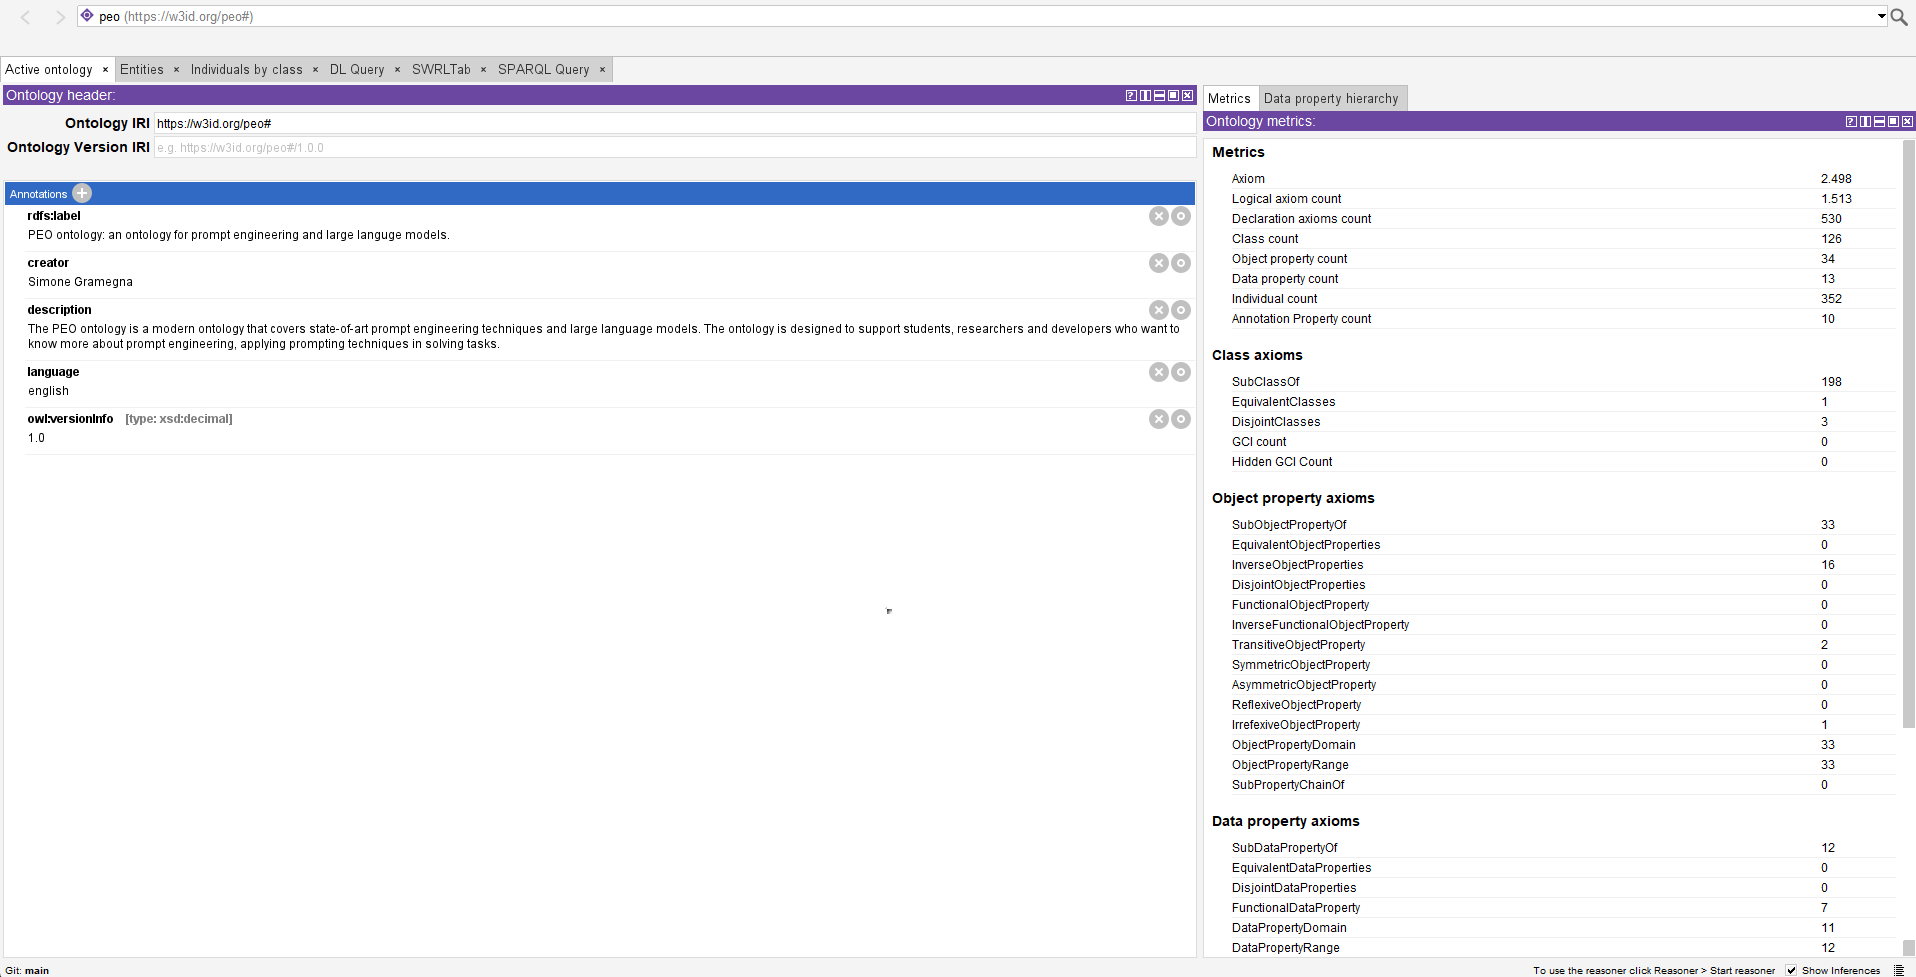
\includegraphics[width=0.8\linewidth]{Figures/fig_29.png}
    \caption{PEO main page}
    \label{fig:29}
\end{figure}
Fig. \ref{fig:29} shows the PEO main page.
Once created the IRI, we define the five annotations and we report them in Tab. \ref{table:t_4_1}. 
\begin{table}[H]
    \footnotesize 
    \centering
    \begin{tabular}{|>{\raggedright\arraybackslash}p{6cm}|>{\raggedright\arraybackslash}p{6cm}|}
        \hline
        Annotation & Annotation value \\ \hline
         rdfs:label & PEO: an ontology for prompt 
         engineering and LLMs. \\ \hline
         
         creator & Simone Gramegna\\ \hline
         
         rdfs:comment & The PEO is a modern ontology that covers state-of-art prompt engineering techniques and LLMs. The ontology is designed to support students, researchers and developers who want to know more about prompt engineering, applying prompting techniques in solving tasks. \\ \hline
         
         language & English \\ \hline
         
         owl:versionInfo & 1.0 \\ \hline
    \end{tabular}
    \caption{Ontology annotations in the main page}
    \label{table:t_4_1}
\end{table}


Starting from the concepts outlined in the conceptualization phase, we define the primary classes of the ontology, which include:
\begin{itemize}
    \item Base model

    \item Capability

    \item Large Language Model

    \item Organization

    \item Prompt engineering

    \item Task
\end{itemize}
All these classes are mutually disjoint, as they represent distinct entities with no overlapping properties.
The only exception is given by "Base model" and "Capability", which are not disjoint.
Both represent attributes of LLMs and are collectively grouped under the "LLM characteristic" class, formed by the union of the two classes. \\
The Capability has five subclasses, each subclass has a label and a comment:
\begin{table}[H]
    \footnotesize 
    \centering
    \begin{tabular}{|>{\raggedright\arraybackslash}p{6cm}|>{\raggedright\arraybackslash}p{6cm}|}
        \hline
        Label & Comment \\ \hline
         Audio processing &  Capability to process audio files. \\ \hline
         
         Code processing & Capability to process source code written in any programming language. \\ \hline
         
         Image processing & Capability to process images, understanding the content of the image. \\ \hline
         
         Text processing & Capability to process text and documents with text inside. \\ \hline
         
         Video processing & Capability to process video files. \\ \hline
    \end{tabular}
    \caption{Capability subclasses}
\end{table}
Each subclass has an individual with the same name, those individuals are created with the aim of assigning a capability to the instances of LLMs that possess it, this aspect will be discussed later.

\subsection{Definition of Large Language Models and their Characteristics}
\label{subsection:4_3_3_llms}
The class "Base model" represents the models at the base of the architecture of LLMs, it has six subclasses each one with label, description and reference.
A subclass can have another subclass representing a more specific architecture, for example the subclass "Decoder" has the subclasses "Decoder only" and "Pixel decoder". 
I have included only the foundational models of the LLMs represented in the ontology, excluding other base models as they fall outside the scope of this ontology.
The subclasses included are: 
\begin{table}[H]
    \footnotesize 
    \centering
    \begin{tabular}{|>{\raggedright\arraybackslash}p{6cm}|>{\raggedright\arraybackslash}p{6cm}|}
        \hline
        Class & Subclasses \\ \hline
         CLIP & none \\ \hline
         
         Decoder & Decoder-only, Pixel decoder \\ \hline
         
         Diffusion model & none \\ \hline
         
         Encoder & Encoder only, Global Image Encoder, Grounding Image Encoder, Region Encoder, ViT Encoder \\ \hline
         
         Recurrent Neural Network & none \\ \hline

        Transformer & Q-Former, LAMDA PT, Transformer XL \\ \hline
    \end{tabular}
    \caption{Base model subclasses}
\end{table}
The class "LLM characteristic" is a subclass of both "Base model" and "Capability".
Each LLM subclass is connected to those two classes using the relations: has\_capability (inverse relation is\_capability) and has\_model\_architecture.
In total there are 33 LLMs subclasses of LLM, each representing a type of LLM such as GPT, Gemini ecc.
The definition of LLMs is completed with a label, a description, a link to the paper, and a link to the website.
Below there are LLMs in PEO with their capabilities and architecture.
\begin{table}[H]
    \footnotesize 
    \centering
    \begin{tabular}{|>{\raggedright\arraybackslash}p{4cm}|>{\raggedright\arraybackslash}p{4cm}|>{\raggedright\arraybackslash}p{4cm}|}
        \hline
        LLM & Capabilities & Base models \\ \hline
        Alpaca & Text processing & Transformer\\ \hline
        BERT & Text processing & Encoder only \\ \hline
        BLIP-2 & Image processing & Q-Former \\ \hline
        BLOOM & Text processing & Transformer \\ \hline
        Chinchilla & Text processing & Transformer \\ \hline
        Claude & Text processing & Transformer \\ \hline
        CogVLM & Image processing & ViT Encoder \\ \hline
        Command R & Text processing & Transformer \\ \hline
        DALL-E & Image processing & CLIP, Decoder, Transformer \\ \hline
        Falcon & Text processing & Decoder only \\ \hline
        FLAN & Text processing & LAMDA PT \\ \hline
        Gemini & Audio processing, Code processing, Image Processing, Text processing, Video processing & Transformer\\ \hline
        Gemma & Text processing & Transformer \\ \hline
        GLaMM & Image processing & Global Image Encoder, Grounding Image Encoder \\ \hline
        LLaMA & Text processing & Transformer \\ \hline
        Midjourney & Image processing & Diffusion model  \\ \hline
        Minerva & Text processing & Transformer \\ \hline
        Mistral & Text processing & Transformer \\ \hline
        MPT-7B & Text processing & Decoder only \\ \hline
        OLMo & Text processing & Decoder only \\ \hline
        OpenELM & Text processing & Decoder only \\ \hline
        OPT & Text processing & Transformer \\ \hline
        PaLM & Text processing, Code processing & Transformer \\ \hline
        Phi-1 & Text processing & Transformer \\ \hline
        RWKV LLM & Text processing & Recurrent Neural Network, Transformer \\ \hline
        Sora & Video processing & Decoder only \\ \hline
        StableLM & Text processing & Decoder only \\ \hline
        StarCoder & Code processing & Decoder only \\ \hline
        T5 & Text processing & Transformer \\ \hline
        VALL-E & Audio processing & Transformer \\ \hline
        Vicuna & Text processing & Transformer \\ \hline
        XLNet & Text processing & Transformer XL \\ \hline
    \end{tabular}
    \caption{Large language models in PEO}
\end{table}
There is a relation based\_on between two subclasses of LLM (with inverse relation basis\_for) where a LLM is developed starting from the base of another LLM.
For example Alpaca is based on LLaMA (another family of LLMs).
Each type of LLM has a capability, this capability is common for all instances of the LLM.
Hence, if a specific version of a LLM has a new capability, the single LLM can be connected to that specific capability. For example, GPT has capability text processing but GPT-3.5 has also the capability of code processing so this version has two capabilities (text processing and code processing).
Same goes for GPT-4 which is an evolution of GPT-3.5 and has also the image processing capability; so it has three capabilities (text processing, code, processing and image processing).
This approach is very flexible because there is no need to divide into categorical classes each version of LLM by simply connecting the version with the specific instance of the capability.
There are three relations between versions of the same LLM: 
\begin{itemize}
    \item has\_variant: relation between two LLMs (x and y), where x has y as another version.

    \item evolves: transitive relation between two LLMs (x and y), where y is an evolution of x. 

    \item evolved\_from: transitive inverse relation of evolves between two LLMs x and y.
\end{itemize}

The relation has\_variant express a different version of the model, while the relation evolves specifies the evolution between two LLMs. 
The latter can also be used to infer the former.
For example, if GPT-3.5 evolves GPT-4 then GPT-3.5 has variant GPT-4.
We use SWRL rules to infer this connection. 
The chosen reasoner is the Hermit reasoner\cite{glimm2014hermit}: a reasoner already included in Protégé which does not require the installation of any additional plug-in.
The reasoner ensures the ontology consistency, inferring new axioms and processing SWRL rules.

SWRL rules are widely applied in PEO.
Firstly, they can infer the relation has\_variant from the relation  evolves. Specifically, the rule is:
\begin{lstlisting}
peo:evolves(?x, ?y) -> peo:has_variant(?x, ?y)
\end{lstlisting}
$?x$ and $?y$ are the two instances involved in the relations.
The rule is applied to all instances that satisfy the condition in the body of the rule.
If a model evolves into another model, the evolved model has the capabilities of the previous model.
This concept is expressed using this SWRL rule:
\begin{lstlisting}
peo:evolves(?x, ?y) ^ peo:has_capability(?x, ?c) -> peo:has_capability(?y, ?c)
\end{lstlisting}
These two relations are not explicitly defined in the ontology, but are inferred by the reasoner.
Each instance of the LLM has two data properties associated 
\begin{itemize}
    \item has\_number\_parameters: number of parameters of the model.

    \item has\_release\_year: year of release of the model
\end{itemize}
Those two data properties are functional, assigning a single value of each property to the instance of the LLM.

Large language models are developed by organizations that can be universities, research institutions and companies for business purpose, the class Organization contains has such three subclasses (with label  and description).
\begin{table}[H]
    \footnotesize 
    \centering
    \begin{tabular}{|>{\raggedright\arraybackslash}p{6cm}|>{\raggedright\arraybackslash}p{6cm}|}
        \hline
        Subclass or organization & Number of entities \\ \hline
        
        University & 2 \\ \hline
 
        Research institution & 8 \\ \hline
        
        Company & 13 \\ \hline
    \end{tabular}
    \caption{Number of organization entities}
\end{table}
Every instance of organization has two associated data properties:
\begin{itemize}
    \item registered\_name: the official name of the organization.

    \item official\_website: the official website of the organization.
\end{itemize}
Organizations and LLMs are connected using the develops relation, connecting an organization with an LLM. 
It is well known that an organization not only develops a single version of an LLM, but the entire family (represented by the different subclasses of the LLM class).
Based on the relation has\_variant, we created the following SWRL rule
\begin{lstlisting}
peo:develops(?c, ?x) ^ peo:has_variant(?x, ?y) -> peo:develops(?c, ?y)    
\end{lstlisting}
If a company $c$ develops a LLM $?x$ and the LLM $x$ has variant another LLM (of the same type) $y$, then the company $c$ develops the llm $y$.
This rule requires that the relationship has\_variant exists among all versions of LLMs or the relation evolves should exist, in order to infer has\_variant.
For example, if OpenAI develops GPT-1, GPT-1 evolves GPT-2 (has variant GPT-2) then OpenAI develops GPT-2.
This process during the inference is automatic because the evolves relation is transitive.

Another SWRL rule that involves the develops relation is the following:
\begin{lstlisting}
peo:is_organization_of(?o1, ?o2) ^ peo:develops(?o1, ?llm) -> peo:develops(?o2, ?llm)
\end{lstlisting}
If an organization $o1$ is organization of another organization $o2$ (for example DeepMind is organization of Google) and $o1$ develops a LLM, then $o2$ develops the LLM.
This is important to specify because several research teams rely on and acknowledge the contribution of other organizations that provides financial support and resources.

\subsection{Definition of Task}
\label{subsection:4_3_4_task}
The Task class represents task that are solved by LLMs applying prompting techniques, there are five specific subclasses representing the different types of task distinguished based on the type of data to process: image, text, video, audio, or code.
Each subclass has other subclasses representing the specific task, e.g., audio generation, text translation ecc as we can see in the table below:
\begin{table}[H]
    \footnotesize 
    \centering
    \begin{tabular}{|>{\raggedright\arraybackslash}p{6cm}|>{\raggedright\arraybackslash}p{6cm}|}
        \hline
        Task type & Subclasses \\ \hline
        Audio task & Audio generation, Audio explanation \\ \hline

        Video task & Video generation, Video explanation \\ \hline
    \end{tabular}
    \caption{Types of task with subclasses - part 1}
\end{table}

\begin{table}[H]
    \footnotesize 
    \centering
    \begin{tabular}{|>{\raggedright\arraybackslash}p{6cm}|>{\raggedright\arraybackslash}p{6cm}|}
        \hline
        Task type & Subclasses \\ \hline
        Code task & Code generation, Code explanation \\ \hline

        Image task & Image generation, Image explanation, Image segmentation \\ \hline

        Text task & Emotion classification, Mathematical understanding, Question-Answering, Text explanation, Test generation, Text summarization, Text translation \\ \hline
    \end{tabular}
    \caption{Types of task with subclasses - part 2}
\end{table}
All of those classes have a label and a description describing shortly the task.
The data property has\_description can be employed for a task to specify its description.

\subsection{Definition of Prompt Engineering}
\label{subsection:4_3_5_prompt}
The Prompt engineering class serves to model all concepts associated with prompts, such as their creation, the context in which they are applied, and the responses they produce.
It has four main subclasses, each one with a label and a description:
\begin{itemize}
    \item Chat: context in which a prompt is created. 
    \item Prompt: input to a LLM.
    \item Prompting technique: technique used to create a prompt.
    \item Response: response given by a LLM after a prompt.
\end{itemize}
The prompting technique is very important because it has all the subclasses representing the different prompting techniques and all instances of those classes are connected using different object properties.
All subclasses of Prompting Technique refer to techniques used in tasks that involve processing only textual content.
Prompting techniques related to images and source code are specifically addressed by their respective class hierarchies based on Code prompting technique and Image prompting techniques.
Prompting techniques for audio and video have not been specified, as the few existing techniques are not yet well-established.
The prompting techniques are gathered from papers, as seen in the background chapter, each subclass representing the specific technique has a label, a description and a reference.
In total there are 24 prompting techniques:
\begin{itemize}
    \item Active prompting 
    \item Analogical prompting
    \item Automatic Chain-of-Thought prompting
    \item Chain-of-Knowledge prompting
    \item Chain-of-Note prompting
    \item Chain-of-Table prompting
    \item Chain-of-Thought prompting
    \item Chain-of-Verification prompting
    \item Decomposed prompting
    \item Emotion prompting
    \item Few shot prompting
    \item Graph of Thoughts prompting
    \item Least-to-most prompting
    \item Logical Chain-of-Thought prompting
    \item ReAct prompting
    \item Retrieval Augmented Generation - RAG prompting
    \item Role prompting
    \item Self consistency prompting
    \item System-2-Attention prompting
    \item Take a step back prompting
    \item Thread of Thought prompting
    \item Tree of Thoughts prompting
    \item Zero shot prompting
\end{itemize}
For code, the class Code Prompting Technique has four subclasses:
\begin{itemize}
    \item Chain-of-Code prompting
    \item Program of Thoughts prompting
    \item Scratchpad prompting
    \item Structured Chain-of-Thought prompting
\end{itemize}
Image prompting technique class has six subclasses:
\begin{itemize}
    \item Fix deformed generations prompting
    \item Lighting
    \item Quality boosters
    \item Repetition
    \item Shot type
    \item Style modifiers
\end{itemize}
To ensure the accurate and consistent representation of prompts generated using the listed techniques, instances of the Prompting Technique class are connected to instances of other Prompt Engineering subclasses via dedicated object properties, defined explicitly or inferred by the reasoner using SWRL rules.
To illustrate all instances along with their associated object properties and data properties, we propose a simple task: translating the phrase "Ciao, come va?" from Italian to English using a zero-shot prompt as input to GPT-4.\\
The first step is to create, if it does not already exist, an instance of the "Text translation" subclass of Task, which we will name "translation\_1" assigning for the data property has\_description the string value: "Translation of the text: Ciao, come va?".
Now I create the instance of the prompting technique that is going to solve the task, in this case we create an instance of the subclass "Zero shot prompting" called "zs\_prompting\_1".
This instance is connected to "translation\_1" using the object property solves\_task with the inverse property "solved\_by" connecting the two instances in both directions. Before creating the prompt, we create an instance of the chat class, calling it "gpt4\_chat\_1" and connecting to the instance GPT-4 of the GPT class using the object property uses\_model with inverse property is\_used\_in\_chat.
The chat instance has three data properties associated:
\begin{itemize}
    \item has\_chat\_title: title of the chat, we assign it "Translation GPT-4 italian to english 1".

    \item start\_time\_chat: start time of the chat, we assign to it the currant time while I'm writing this chapter: "29/11/2024 - 10:37"

    \item end\_time\_chat: end time of the chat, the chat has the duration of two minutes and I assign the value: "29/11/2024 - 10:39"
\end{itemize}
Obviously those example values can be modified later.
Now that a context is established, the chat "gpt4\_chat\_1", we proceed to create the instance of the Prompt.
We specify that the prompt called "zs\_1" is created using the instance of Zero shot prompting previously defined using the object property prompt\_generated\_using with inverse property is\_used\_in\_prompt, in our case "zs\_1" is generated using "zs\_prompting\_1".
A prompt instance can have three associated data properties:
\begin{itemize}
    \item has\_instruction: main instruction of the prompt.

    \item has\_input\_data: data given as input to the prompt. 

    \item has\_output\_indicator: indicator that indicates the format of the response.
\end{itemize}
For simplicity, we assign the instruction "Translate the English text to Italian, the input Text: Ciao, come va?  and the output format: Translation:  to the prompt, other data properties values can be added later.
Now we connect the prompt with its context, the "gpt4\_chat\_1" using the object property has\_context with inverse relation has\_prompt and after the creation of this relation using a SWRL rule I connect the prompt with the LLM that takes it in input. 
\begin{lstlisting}
peo:has_context(?p, ?c) ^ peo:uses_model(?c, ?m) -> peo:processed_by(?p, ?m)   
\end{lstlisting}
If the context of a prompt $p$ is a chat $c$, which uses the LLM $m$, then $p$ is processed by the LLM $m$.
This rule creates automatically during the reasoning the relation processed\_by with inverse relation processes.

After a prompt, the LLM generates a response, which in PEO is instance of the Response class.
The value is associated using the data property has\_response\_value and is connected to the prompt that generated it using the object property response\_followedby\_prompt.
In order to model the "chain" prompt-responses-prompt, I created the following object properties:
\begin{itemize}
    \item response\_followedby\_prompt: the response is after a prompt.

    \item prompt\_follows\_response: after the prompt there is a response, inverse property of response\_followedby\_prompt.

    \item prompt\_follows\_prompt: after the prompt there is another prompt.

    \item prompt\_followedby\_prompt: before the prompt there is another prompt, inverse property of {prompt\_follows\_prompt}.

    \item response\_follows\_prompt: after the response there is a prompt.

    \item prompt\_followedby\_response: before the prompt there is a response, inverse relation of response\_follows\_prompt. 
\end{itemize}
We can graphically see this concatenation in the following scheme:
\begin{figure}[H]
    \centering
    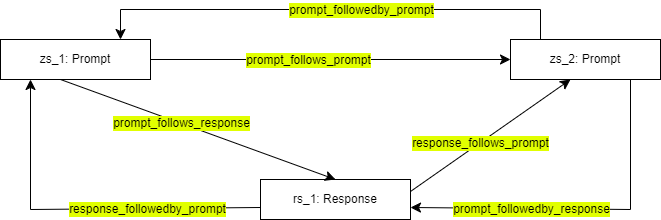
\includegraphics[width=0.9\linewidth]{Figures/fig_30.png}
    \caption{Chain prompt-response}
    \label{fig:enter-label}
\end{figure}
Of course, most of these relationships are automatically created during the inference process.
To connect a response with the next prompt, we created this SWRL rule:
\begin{lstlisting}
peo:prompt_followedby_prompt(?x, ?y) ^ peo:prompt_follows_response(?y, ?r) -> peo:prompt_followedby_response(?x, ?r)
\end{lstlisting}
It states that if a prompt $?x$ is followed by another prompt $?y$ and $?y$ has a response $?r$, then $?x$ is followed by $?r$.

The context of the next prompt is assigned automatically using the object property prompt\_followedby\_prompt and this SWRL rule:
\begin{lstlisting}
peo:prompt_followedby_prompt(?x, ?y) ^ peo:has_context(?y, ?c) -> peo:has_context(?x, ?c)
\end{lstlisting}
It states that if a prompt $x$ is followed by another prompt $y$ and $y$ is connected to the chat $c$ as context, then $x$ has context $c$.
Also, each response is connected the chat using the object property is\_response\_of (inverse property has\_response) created using the SWRL rule:
\begin{lstlisting}
peo:response_followedby_prompt(?r, ?p) ^ peo:has_context(?p, ?c) -> peo:is_response_of(?r, ?c)
\end{lstlisting}
It states that if a response $?r$ is followed by a prompt $?p$, which is connected to the chat $c$ as context, then the response $?r$ is the response of $?c$.
The last SWRL rule connects the response with the model that has generated it creating the object property response\_generated\_using with the inverse property generates\_response:
\begin{lstlisting}
peo:response_followedby_prompt(?r, ?p) ^ peo:processed_by(?p, ?m) -> peo:response_generated_using(?r, ?m) 
\end{lstlisting}
It states that if a response $?r$ is followed by a prompt $?p$ and the prompt $?p$ is processed by the LLM $?m$, then the response $?r$ is generated using $?m$.
\begin{figure}[H]
    \centering
    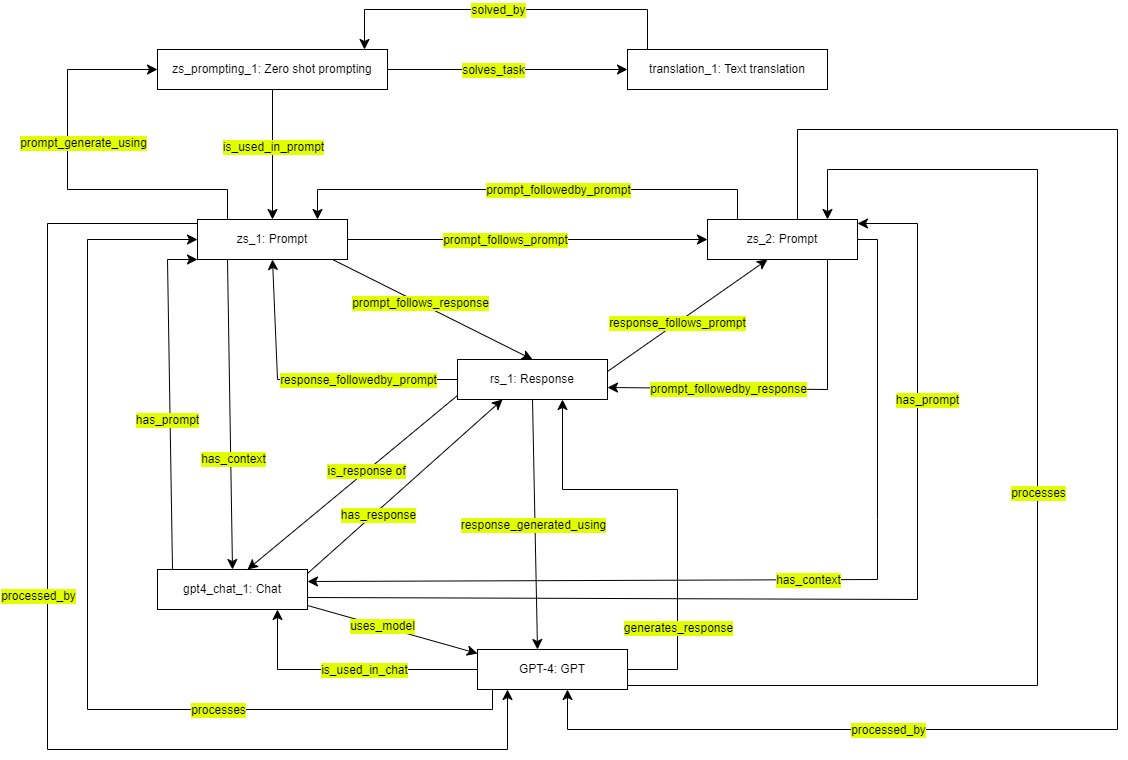
\includegraphics[width=0.85\linewidth]{Figures/fig_31.png}
    \caption{Chat scheme}
    \label{fig:31}
\end{figure}
Fig.~\ref{fig:31} further clarifies the aforementioned object properties.

\subsection{Population}
\label{subsection:4_3_6_population}
Populating the ontology with prompts is a complex process as it requires connecting various instances (task, prompting technique, prompt, chat, response, LLM) using the defined object properties. Moreover, each prompt is manually crafted in accordance with the specific prompting technique.
Manually populating the ontology with all instances for every task, every version of each LLM, and every prompting technique would be highly time-consuming and beyond the objectives of this thesis.
Therefore, we focus on a specific subset of the ontology: LLMs, tasks, prompting techniques, and prompts.
The LLMs are very popular ones available to the users, namely:
\begin{itemize}
    \item GPT-4
    \item Mistral-7B
    \item Gemini Flash
\end{itemize}
Moreover, the following prompting techniques are considered:
\begin{itemize}
    \item Zero-shot prompting: allows LLMs to handle new tasks using only natural language instructions, without requiring examples or any effort by the user.

    \item Few-shot prompting: enables language models to learn new tasks with few examples, reducing the need for extensive task-specific datasets.
    
    \item Role prompting: improves LLMs performance on solving tasks by simulating specific roles.

    \item Emotion prompting:  enhances LLMs by integrating emotions into prompts, improving response generation and performance on tasks.

    \item Analogical prompting: is able to generate automatically task-specific exemplars, reducing manual annotation needs, and improving performance on problem-solving tasks.
\end{itemize}
Finally, the following four tasks are considered:
\begin{itemize}
    \item Emotion classification: classification of the emotion in a given text.

    \item Mathematical understanding: solving a given mathematical problem of medium difficulty. 

    \item Text translation: translation of a text from English to Italian.

    \item Text summarization: summarization of the content of a given text.
\end{itemize}

Below, we list the prompts created for each task and for each prompting technique.\\\\
Task 1: Emotion classification\\     
The input text to be classified is: "I think the vacation is okay"
\begin{itemize}
    \item Zero-shot prompting: Classify the text into neutral, negative or positive. Text: "I think the vacation is okay." Sentiment:
    \item Few-shot prompting: Classify the following text into neutral, negative, or positive based on its sentiment. Here are some examples: 
    Text: "The food was absolutely wonderful!" Sentiment: Positive. 
    Text: "I did not enjoy the movie at all." Sentiment: Negative. 
    Text: "It was an average experience." Sentiment: Neutral. 
    Now, classify this text: Text: "I think the vacation is okay." Sentiment:
    \item Emotion prompting: Classify the following text into neutral, negative, or positive based on its sentiment. This task is very important to my career. Please provide a well-thought and accurate classification. Text: "I think the vacation is okay." Sentiment:
    \item Role prompting: From now on, you are an experienced sentiment analyst with deep expertise in understanding human emotions through textual analysis. Your task is to classify the sentiment of texts as neutral, negative, or positive with utmost accuracy and professionalism. Text: "I think the vacation is okay." Sentiment:
    \item Analogical prompting: Classify the text into neutral, negative or positive. \# Instruction: \# Text: I think the vacation is okay. \# Sentiment:
\end{itemize}
Task 2: Mathematical understanding\\
For the mathematical understanding there is the solving of a simple geometrical problem: the calculation of a square with the four vertices at (-2, 2), (2, -2), (-2, -6), and (-6, -2). 
\begin{itemize}
    \item Zero-shot prompting: What is the area of the square with the four vertices at $(-2, 2)$, $(2, -2)$, $(-2, -6)$, and $(-6, -2)$?
    \item Few-shot prompting: Instruction: Determine the area of a square given the coordinates of its four vertices. 
    Example 1: Vertices: $(0, 0)$, $(4, 0)$, $(4, 4)$, $(0, 4)$ 
    Step 1: Identify the side length. Distance between $(0, 0)$ and $(4, 0)$ is $\sqrt{((4 - 0)^2 + (0 - 0)^2)} = 4$. 
    Step 2: Calculate the area. Area = side length$^2 = 4^2 = 16$. Answer: 16. 
    Example 2: Vertices: $(-1, 1)$, $(-1, 3)$, $(1, 3)$, $(1, 1)$ 
    Step 1: Identify the side length. Distance between $(-1, 1)$ and $(-1, 3)$ is $\sqrt{((3 - 1)^2 + (1 - 1)^2)} = 2$. 
    Step 2: Calculate the area. Area = side length$^2 = 2^2 = 4$. Answer: 4. 
    Query: Vertices: $(-2, 2)$, $(2, -2)$, $(-2, -6)$, $(-6, -2)$. 
    Step 1: Identify the side length by calculating the distance between consecutive vertices. 
    Step 2: Calculate the area of the square. Answer:
    \item Emotion prompting: Please calculate the area of a square given the coordinates of its vertices. This task is important for building my understanding of geometry and improving my analytical skills, so I truly value a thorough and accurate solution. Vertices: $(-2, 2)$, $(2, -2)$, $(-2, -6)$, $(-6, -2)$.
    \item Role prompting: From now on, you are a brilliant geometry teacher. You always explain geometry problems thoroughly and ensure your students understand every step of the process. We have a question for you: I have four vertices of a square: $(-2, 2)$, $(2, -2)$, $(-2, -6)$, and $(-6, -2)$. Can you help me calculate the area of the square step by step? Please provide a detailed explanation of how to verify the shape, calculate the side length, and determine the area.
    \item Analogical prompting: What is the area of the square with the four vertices at $(-2, 2)$, $(2, -2)$, $(-2, -6)$, and $(-6, -2)$? \# Instruction: \#\# Recall relevant exemplars: \#\# Solve the initial problem:
\end{itemize}
Task 3: Text translation\\
For text translation task I chosed a citation of Lewis Carol \cite{carol} to translate form english to italian: "Sometimes, we've believed as many as six impossible things before breakfast."
\begin{itemize}
    \item Zero-shot prompting: Translate the English text to Italian. Text: "Sometimes, we've believed as many as six impossible things before breakfast." Translation:
    \item Few-shot prompting: Translate the following English sentences into Italian: 
    1. English: "Sometimes, we've believed as many as six impossible things before breakfast." Italian: "A volte, ho creduto a ben sei cose impossibili prima di colazione." 
    2. English: "I think, therefore I am." Italian: "Penso, quindi sono." 
    3. English: "All the world's a stage, and all the men and women merely players." Italian: "Tutto il mondo è un palcoscenico e tutti gli uomini e le donne sono solo attori." 
    Now translate this sentence: English: "Sometimes, we've believed as many as six impossible things before breakfast." Italian:
    \item Emotion prompting: Translate the following text to Italian. It's very important for me to understand this translation accurately as it could affect my professional progress: "Sometimes, we've believed as many as six impossible things before breakfast."
    \item Role prompting: From now on, you are an excellent literary translation teacher who accurately explains the meaning and tone of complex sentences. Translate the following sentence from English to Italian, preserving its meaning and tone: "Sometimes, we've believed as many as six impossible things before breakfast."
    \item Analogical prompting: \# Problem: "Sometimes, we've believed as many as six impossible things before breakfast." 
    \# Relevant Problems: 
    1. Translating a complex sentence from English to Italian. 
    - Question: How to translate the sentence "To be or not to be, that is the question" into Italian? 
    - Answer: The sentence "To be or not to be, that is the question" translates into Italian as "Essere o non essere, questo è il problema." 
    2. Translating a sentence with idiomatic expressions. 
    - Question: How to translate "Break a leg!" into Italian? 
    - Answer: The idiomatic expression "Break a leg!" translates into Italian as "In bocca al lupo!" 
    3. Translating a sentence with abstract concepts. 
    - Question: How to translate "The only limit is your imagination" into Italian? 
    - Answer: The sentence "The only limit is your imagination" translates into Italian as "L'unico limite è la tua immaginazione." 
    \# Translation of the initial problem: The sentence "Sometimes, we've believed as many as six impossible things before breakfast" translates into Italian as:
\end{itemize}
Task 4: Text summarization\\
The last task is the summarization of the following text about permaculture: "Permaculture is a design process mimicking the diversity, functionality and resilience of natural ecosystems. The principles and practices are drawn from traditional ecological knowledge of indigenous cultures combined with modern scientific understanding and technological innovations. Permaculture design provides a framework helping individuals and communities develop innovative, creative and effective strategies for meeting basic needs while preparing for and mitigating the projected impacts of climate change."\cite{permaculture}
\begin{itemize}
    \item Zero-shot prompting: Permaculture is a design process mimicking the diversity, functionality and resilience of natural ecosystems. The principles and practices are drawn from traditional ecological knowledge of indigenous cultures combined with modern scientific understanding and technological innovations. Permaculture design provides a framework helping individuals and communities develop innovative, creative and effective strategies for meeting basic needs while preparing for and mitigating the projected impacts of climate change. Write a summary of the above text. Summary:
    \item Few-shot prompting: You are an expert at creating concise summaries. Below are some examples of summaries based on texts.
    Example 1: Text: The Earth orbits the Sun in an elliptical pattern, taking approximately 365.25 days to complete one orbit. This forms the basis of the Gregorian calendar year. Summary: The Earth completes an orbit around the Sun in roughly 365 days, defining the calendar year.
    Example 2: Text: Sustainable agriculture incorporates practices that maintain productivity and minimize environmental impact, such as crop rotation and organic farming. Summary: Sustainable agriculture uses eco-friendly practices like crop rotation and organic methods to maintain productivity.
    Task: Text: Permaculture is a design process mimicking the diversity, functionality, and resilience of natural ecosystems. The principles and practices are drawn from traditional ecological knowledge of indigenous cultures combined with modern scientific understanding and technological innovations. Permaculture design provides a framework helping individuals and communities develop innovative, creative, and effective strategies for meeting basic needs while preparing for and mitigating the projected impacts of climate change. Summary:
    \item Emotion prompting: Summarize the essence of permaculture, focusing on its innovative design process inspired by natural ecosystems. Highlight how it combines traditional ecological knowledge with modern science and technology to address climate change. This understanding is vital to my research and the future of sustainable living. Please ensure the summary is concise yet comprehensive.
    \item Role prompting: From now on, you are an environmental scientist who specializes in explaining complex ecological concepts in an accessible and engaging manner. Your task is to provide a concise summary of permaculture principles and their importance in addressing climate challenges.
    \item Analogical prompting: Problem: Summarize the definition and essence of permaculture using principles that mirror natural ecosystems and combine traditional ecological knowledge with modern science. Instruction: Recall three relevant and distinct problems or topics related to summarizing processes that focus on mimicking complex systems. Provide detailed exemplars for each recalled instance, including how the principles were extracted and utilized effectively. Use the recalled insights to structure and write the final summary.
\end{itemize}
The responses for each prompt from the three LLMs have been saved in the ontology, and a chat has been created for each prompt, including a title, start time, and end time resulting in a total of 60 distinct chats.
\begin{figure}[H]
    \centering
    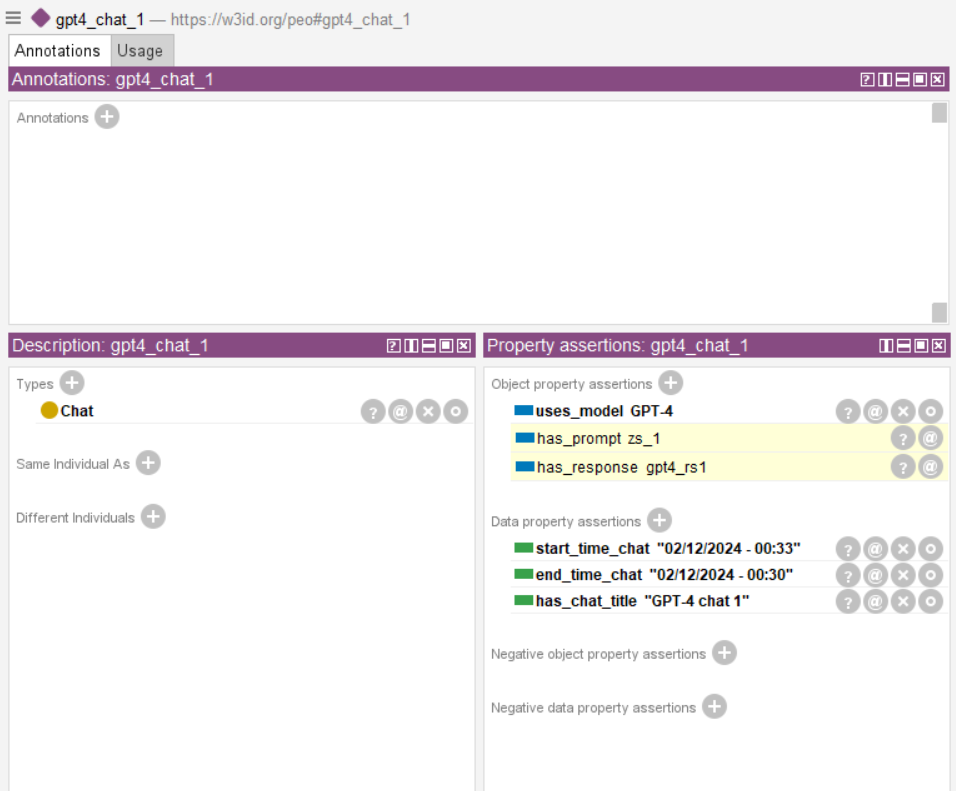
\includegraphics[width=0.75\linewidth]{Figures/fig_32.png}
    \caption{Example of chat with relations inferred}
    \label{fig:enter-label}
\end{figure}

\subsection{Automatic Population}
\label{subsection:4_3_7_automatic}
Populating an ontology with various instances can be a time-consuming task for developers, as the ontology's domain of interest often involves numerous entities requiring manual insertion.
To streamline this process automation can be employed.
The methodology proposed in \cite{norouzi2024ontology} allows to semi-automatically populate modular ontologies using LLMs.
It focuses on leveraging the strengths of LLMs, such as GPT-4 and Llama-3, for extracting structured knowledge from natural language texts.
The method is divided into three main stages: data preprocessing, relevant text retrieval, and ontology population.
In the first stage, the data is cleaned, organized, and aligned with simplified ontology modules to facilitate processing.
The second stage employs text summarization and Retrieval-Augmented Generation (RAG) techniques to identify and extract relevant information aligned with the ontology schema.
Finally, in the third stage, predefined module files guide the LLMs to populate the ontology with accurate triples by using structured prompts.
Despite the good results, the methodology still requires effort, as documents need to be selected and preprocessed to create a dataset that serves as input for the LLM used to populate the ontology. Implementing this process demands skills that go beyond those of an ontology engineer, effectively shifting the workload to another task.\\ 

Moreover, the approach proposed in \cite{saetia2024financial} leverages LLMs, such as GPT-3.5 and GPT-4, to populate financial ontologies by extracting structured data from unstructured texts.
It combines several prompting techniques to improve accuracy and scalability.
Few-shot prompting provides positive and negative examples, whilst Chain-of-Thought (CoT) reasoning encourages step-by-step problem solving,
Moreover, schema.org definitions are included to contextualize fields and properties.
Prompts are carefully designed to generate structured outputs in JSON format for easy integration and evaluating performance using F1 scores, with the best results achieved when combining examples, CoT, and definitions.
Like the previous one, this approach requires considerable effort on gathering necessary docs to pre-process.
Moreover, the quality of the output depends on the prompts.\\
Since our goal in populating the ontology is a set of individuals and triples that is sufficient for the evaluation phase rather than the full range of knowledge, we employ a straightforward ad-hoc approach.
Starting from the sixteen CQs defined in the Ontology requirements specification section, we input them, along with the ontology TBox, into a LLM to generate an automatically populated version of the prompt engineering ontology.
The LLM chosed is GPT-4o: the latest and most powerful version of GPT available in its web interface ChatGPT and used previously in the manual ontology population.
This time instead of giving as input a specific prompt created with one of prompt engineering techniques, we write this prompt, providing the ontology and a text file containing the competency questions.
\begin{figure}[H]
    \centering
    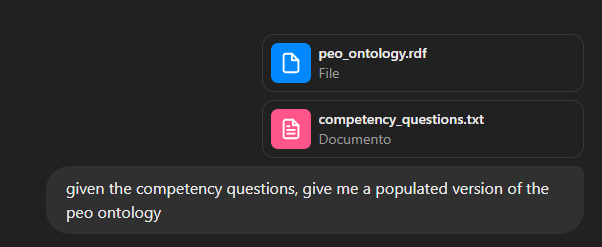
\includegraphics[width=0.9\linewidth]{Figures/fig_34.png}
    \caption{Prompt for automatic ontology population}
    \label{fig:34}
\end{figure}
After this prompt the LLM begins a reasoning process, first it explains the approach followed by the model:
\begin{figure}[H]
    \centering
    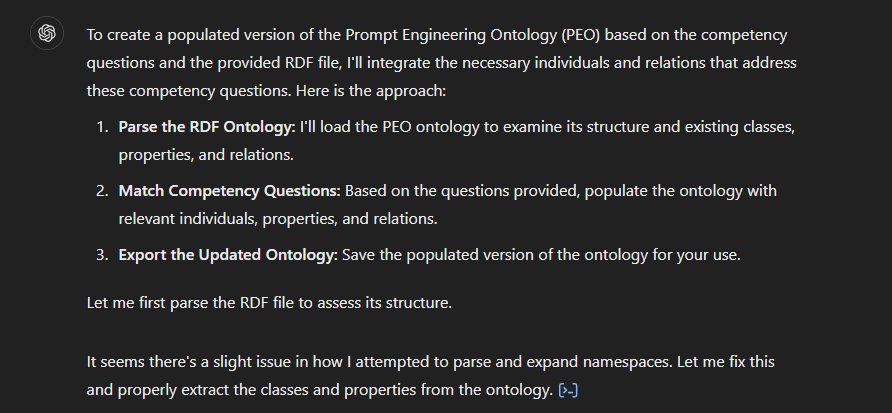
\includegraphics[width=0.9\linewidth]{Figures/fig_35.png}
    \caption{First GPT-4 output in the automatic population}
    \label{fig:enter-label}
\end{figure}
Then the model analyses the ontology structure encoded in the RDF file, listing simple classes and sample object properties found:
\begin{figure}[H]
    \centering
    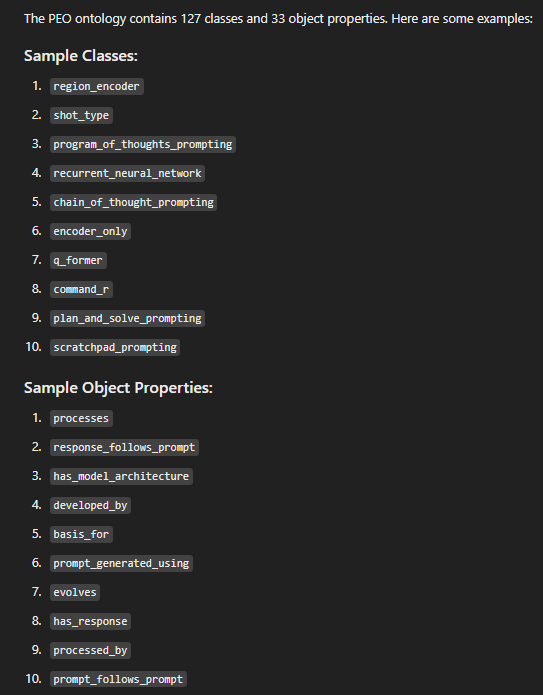
\includegraphics[width=0.85\linewidth]{Figures/fig_36.png}
    \caption{Structure analysis of the ontology}
    \label{fig:enter-label}
\end{figure}
Finally it produces the downloadable RDF file containing the ontology populated by the model.
\begin{figure}[H]
    \centering
    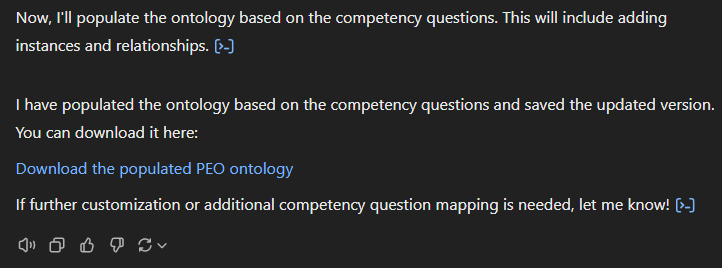
\includegraphics[width=0.9\linewidth]{Figures/fig_37.png}
    \caption{Final LLM output}
    \label{fig:37}
\end{figure}
Fig. \ref{fig:37} shows the final LLM output.
After downloading the RDF file, we open it using the Protegé editor to check the final result.
At a first glance, the obtained result seems rather poor, as four new classes have been created again without considering the classes already present in the ontology:
\begin{itemize}
    \item PromptEngineering
    \item Prompt
    \item PromptingTechnique
    \item Task
\end{itemize}
The class hierarchy is disregarded too as shown in Fig. \ref{fig:38}
\begin{figure}[H]
    \centering
    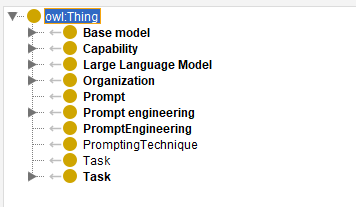
\includegraphics[width=0.9\linewidth]{Figures/fig_38.png}
    \caption{PEO populated automatically}
    \label{fig:38}
\end{figure}
Just two classes have a definition: Prompt and PromptEngineering with no individuals created while the PromptingTechnique class has no defintion and three individuals created:
\begin{itemize}
    \item ChainOfThoughtPrompting
    \item FewShotPrompting
    \item ZeroShotPrompting
\end{itemize}
There is no new instance of chat and all the mechanism defined to link a prompting technique with a chat is completely ignored.
No new object properties or data properties have been created by GPT-4o, just an annotation property called hasDefinition. Any other useful information is not created, the three entities are not linked with any object property and they do not have any data property. Additional prompts would clearly be needed as input for the LLM to improve the result, which is currently poor and adds no useful information compared to the original, manually populated version of the prompt engineering ontology.

\chapter{Experimental Evaluation, Publication, and Maintenance}
\label{chapter:5_evaluation}

This Chapter reports the evaluation process of PEO. Sect. \ref{section:5_1_consistency} discusses the process of the ontology consistency check,
sect. \ref{section:5_2_ontometrics} measures ontology metrics , sect. \ref{section:5_3_oops} detects pitfall in PEO and sect. \ref{section:5_4_cqs} checks the execution of translated competency questions. In the final part of the chapter, sect. \ref{section:5_5_publication} discuss the publication and sect. \ref{section:5_6_discussion} discusses results obtained during the experimental evaluation.

\section{Ontology Consistency Check}
\label{section:5_1_consistency}
The ontology consistency check is a reasoning task available in OWL, and consequently Protege, that assesses the consistency of the ABox with respect to the TBox.
Hence, we execute the reasoner available in Protege that performs such check as well as other reasoning services including the rule-based inference.
We specifically adopt the HermiT reasoner.
Moreover, we consider both the manually populated and the automatic populate ontology.
On the original version of the PEO, the reasoner does not give any inconsistency and all the axioms are inferred correctly.
\begin{figure}[H]
    \centering
    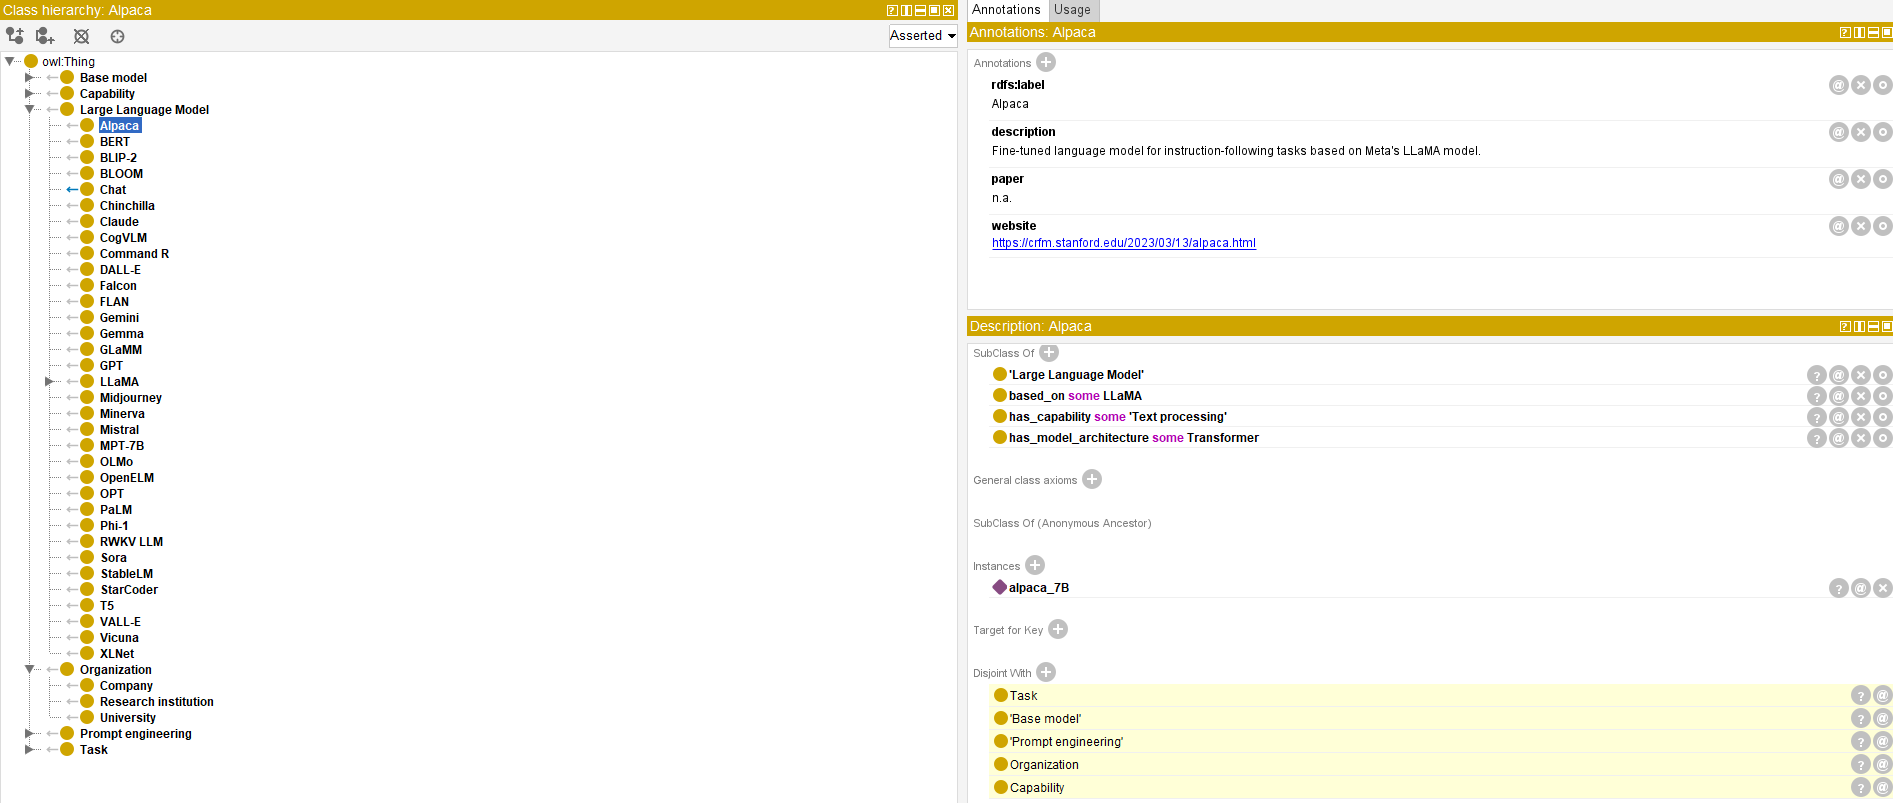
\includegraphics[width=0.9\linewidth]{Figures/fig_39.png}
    \caption{PEO with HermiT reasoner}
    \label{fig:39}
\end{figure}
Fig. \ref{fig:39} shows the execution of HermiT reasoner on PEO.
The reasoner infers correctly that the class "Alpaca" is disjoint with the classes "Task", "Base model", "Prompt engineering", "Organization" and "Capability" because the superclass "Large language model" is declared disjoint with that list of classes.
The ten SWRL rules declared work properly and infer the correct object properties for individuals:
\begin{figure}[H]
    \centering
    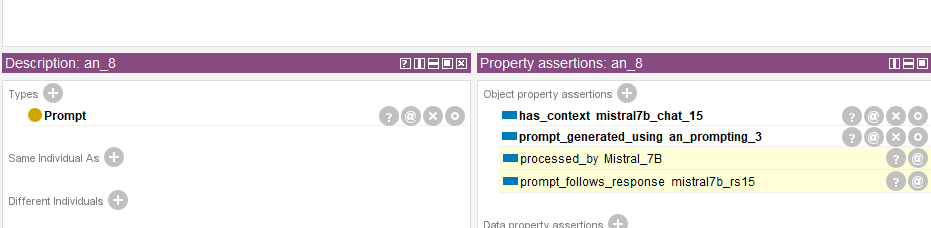
\includegraphics[width=0.9\linewidth]{Figures/fig_40.png}
    \caption{Inference on prompt individual}
    \label{fig:40}
\end{figure}
The consistency check of the other version of the PEO, the one populated using GPT-4 has given the exact results,  because as said in the previous section no additional significant information has been added to the ontology.
The classes added by GPT-4 have no link with the other existing classes and thus they do not lead to new inferences.

\section{OntoMetrics}
\label{section:5_2_ontometrics}
Moreover, we evaluated PEO based on OntoMetrics: a web-based tool developed by the University of Rostock that validates and provides statistical analyses of ontologies \cite{lantow2016ontometrics}.
Given the ontology in form of RDF file or code, it calculates automatically:
\begin{itemize}
    \item Base metrics: these include simple counts of ontology elements such as classes, axioms, and objects, providing a quantitative overview of the ontology's components.

    \item Schema Metrics: these metrics evaluate the structure of the ontology's schema, considering aspects like attribute richness and inheritance richness.

    \item Knowledge base Metrics: these assess the ontology's knowledge base, focusing on the population of instances within the ontology.

    \item Class Metrics: these metrics analyse individual classes within the ontology, examining factors such as class connectivity and fullness.

    \item Graph Metrics: these evaluate the ontology's taxonomy as a graph, measuring properties like depth and breadth.
\end{itemize}
For PEO, I will calculate base metrics, schema metrics and graph metrics.
\begin{figure}[H]
    \centering
    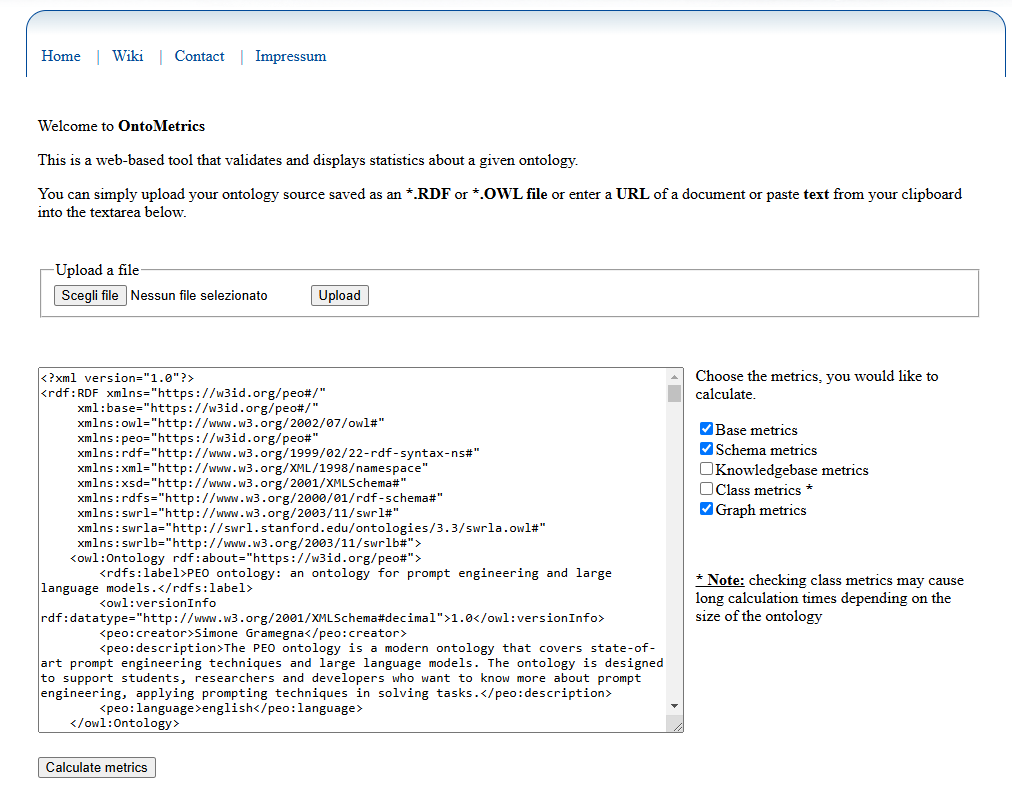
\includegraphics[width=0.9\linewidth]{Figures/fig_41.png}
    \caption{OntoMetrics interface}
    \label{fig:enter-label}
\end{figure}

The values computed for base metrics are reported in Tab.~\ref{tab:base_metrics_peo}.

\begin{table}[H]
    \footnotesize 
    \centering
    \begin{tabular}{|>{\raggedright\arraybackslash}p{8cm}|>{\raggedright\arraybackslash}p{4cm}|}
        \hline
        Property & Value \\ \hline
        Axioms & 2684 \\ \hline
        Logical axioms count & 1695 \\ \hline
        Class count & 126 \\ \hline
        Total classes count & 126 \\ \hline
        Object property count & 34 \\ \hline
        Total object properties count & 34 \\ \hline
        Data property count & 13 \\ \hline
        Total data properties count & 13 \\ \hline
        Properties count & 47 \\ \hline
        Individual count & 352 \\ \hline
        Total individuals count & 352 \\ \hline
        DL expressivity & SRIF(D) \\ \hline
    \end{tabular}
    \caption{PEO base metrics statistics}
    \label{tab:base_metrics_peo}
\end{table}
This table provides a high-level overview of the ontology’s structure and complexity.
With 2684 axioms, the ontology is rich in detail and represents a substantial body of knowledge.
Among these, 1695 logical axioms indicate a strong focus on enabling inference and reasoning.
The 126 classes show that the ontology has a robust framework for organizing concepts, while 34 object properties and 13 data properties highlight the ontology’s emphasis on relationships over attribute-driven modelling.
The inclusion of 352 individuals suggests that the ontology is well-populated, demonstrating practical applicability.
The expressivity of $SRIF(D)$ indicates that the ontology supports features like inverse roles and data ranges, balancing computational efficiency with expressive capability.
This ontology is comprehensive, but may require optimization to handle its inherent complexity effectively.

\begin{table}[H]
    \footnotesize 
    \centering
    \begin{tabular}{|>{\raggedright\arraybackslash}p{8cm}|>{\raggedright\arraybackslash}p{4cm}|}
        \hline
        Class Axiom Type & Count \\ \hline
        SubClassOf axioms count & 199 \\ \hline
        Equivalent classes axioms count & 1 \\ \hline
        Disjoint classes axioms count & 3 \\ \hline
        GCICount & 0 \\ \hline
        HiddenGCICount & 0 \\ \hline
    \end{tabular}
    \caption{PEO Class Axioms statistics}
    \label{tab:class-axioms_peo}
\end{table}
The table \ref{tab:class-axioms_peo} contains the count of the different class axiom types. 
There are one hundred ninety-nine SubClassOf axioms, there is just one Equivalent class axiom and there are three Disjoint classes axioms.
The Global Cardinality Restrictions count (GCICount) and Hidden Global Cardinality Restrictions count (HiddenGCICount) are both equal to zero. Those two indicators equal to zero mean that there are not explicit and implicit global cardinality restrictions.

\begin{table}[H]
    \footnotesize 
    \centering
    \begin{tabular}{|>{\raggedright\arraybackslash}p{8cm}|>{\raggedright\arraybackslash}p{4cm}|}
        \hline
        Object Property Axiom Type & Count \\ \hline
        SubObjectPropertyOf axioms count & 33 \\ \hline
        Equivalent object properties axioms count & 0 \\ \hline
        Inverse object properties axioms count & 16 \\ \hline
        Disjoint object properties axioms count & 0 \\ \hline
        Functional object properties axioms count & 0 \\ \hline
        Inverse functional object properties axioms count & 0 \\ \hline
        Transitive object property axioms count & 2 \\ \hline
        Symmetric object property axioms count & 0 \\ \hline
        Asymmetric object property axioms count & 0 \\ \hline
        Reflexive object property axioms count & 0 \\ \hline
        Irreflexive object property axioms count & 1 \\ \hline
        Object property domain axioms count & 33 \\ \hline
        Object property range axioms count & 33 \\ \hline
        SubPropertyChainOf axioms count & 0 \\ \hline
    \end{tabular}
    \caption{PEO Object Property Axioms Statistics}
    \label{tab:object-property-axioms_peo}
\end{table}
The table \ref{tab:object-property-axioms_peo} contains object property axiom types count in PEO.
There are thirty-three SubObjectPropertyOf axioms, while no Equivalent object properties or Disjoint object properties axioms are present. Additionally, the ontology includes 16 Inverse object properties axioms and two Transitive object property axioms.
Furthermore, no Functional, Inverse functional, Symmetric, or Asymmetric object property axioms are defined. There is also no Reflexive object property axiom, whereas one Irreflexive object property axiom is present.Regarding domain and range definitions, the ontology contains thirty-three Object property domain axioms and 33 Object property range axioms. Lastly, there are no SubPropertyChainOf axioms.


\begin{table}[H]
    \footnotesize 
    \centering
    \begin{tabular}{|>{\raggedright\arraybackslash}p{8cm}|>{\raggedright\arraybackslash}p{4cm}|}
        \hline
        Data Property Axiom Type & Count \\ \hline
        SubDataPropertyOf axioms count & 12 \\ \hline
        Equivalent data properties axioms count & 0 \\ \hline
        Disjoint data properties axioms count & 0 \\ \hline
        Functional data property axioms count & 7 \\ \hline
        Data property domain axioms count & 11 \\ \hline
        Data property range axioms count & 12 \\ \hline
    \end{tabular}
    \caption{PEO Data Property Axioms Statistics}
    \label{tab:data-property-axioms_peo}
\end{table}
Table \ref{tab:data-property-axioms_peo} presents the count of different data property axiom types in PEO. Specifically, there are twelve SubDataPropertyOf axioms, while no Equivalent data properties or Disjoint data properties axioms are present. Additionally, the ontology includes seven Functional data property axioms. Regarding domain and range definitions, the ontology contains eleven Data property domain axioms and twelve Data property range axioms.

\begin{table}[H]
    \footnotesize 
    \centering
    \begin{tabular}{|>{\raggedright\arraybackslash}p{8cm}|>{\raggedright\arraybackslash}p{4cm}|}
        \hline
        Individual Axiom Type & Count \\ \hline
        Class assertion axioms count & 352 \\ \hline
        Object property assertion axioms count & 390 \\ \hline
        Data property assertion axioms count & 580 \\ \hline
        Negative object property assertion axioms count & 0 \\ \hline
        Negative data property assertion axioms count & 0 \\ \hline
        Same individuals axioms count & 0 \\ \hline
        Different individuals axioms count & 0 \\ \hline
    \end{tabular}
    \caption{PEO Individual Axioms Statistics}
    \label{tab:individual-axioms_peo}
\end{table}
Table \ref{tab:individual-axioms_peo} presents the count of different individual axiom types in PEO. Specifically, there are three hundred fifty-two Class assertion axioms, three hundred ninety Object property assertion axioms, and five hundred eighty Data property assertion axioms. Additionally, there are no Negative object property assertion axioms, Negative data property assertion axioms, Same individuals axioms, or Different individuals axioms in the ontology.


\begin{table}[H]
    \footnotesize 
    \centering
    \begin{tabular}{|>{\raggedright\arraybackslash}p{8cm}|>{\raggedright\arraybackslash}p{4cm}|}
        \hline
        Annotation Axiom Type & Count \\ \hline
        Annotation axioms count & 5 \\ \hline
        Annotation assertion axioms count & 459 \\ \hline
        Annotation property domain axioms count & 0 \\ \hline
        Annotation property range axioms count & 0 \\ \hline
    \end{tabular}
    \caption{PEO Annotation Axioms Statistics}
    \label{tab:annotation-axioms_peo}
\end{table}
Table \ref{tab:annotation-axioms_peo} presents the count of different annotation axiom types in PEO. Specifically, there are five Annotation axioms and four hundred fifty-nine Annotation assertion axioms. Additionally, there are no Annotation property domain axioms or Annotation property range axioms in the ontology.


\begin{table}[H]
    \footnotesize 
    \centering
    \begin{tabular}{|>{\raggedright\arraybackslash}p{8cm}|>{\raggedright\arraybackslash}p{4cm}|}
        \hline
        Metric & Value \\ \hline
        Attribute richness & 0.103175 \\ \hline
        Inheritance richness & 1.579365 \\ \hline
        Relationship richness & 0.160338 \\ \hline
        Attribute class ratio & 0.0 \\ \hline
        Equivalence ratio & 0.007937 \\ \hline
        Axiom/class ratio & 21.301587 \\ \hline
        Inverse relations ratio & 0.390244 \\ \hline
        Class/relation ratio & 0.531646 \\ \hline
    \end{tabular}
    \caption{PEO Schema Metrics}
    \label{tab:ontology-metrics_peo}
\end{table}
Table \ref{tab:ontology-metrics_peo} presents the schema metrics for PEO. The Attribute richness is approximately zero point one, while the Inheritance richness is around one point six. The Relationship richness is about zero point one six. The Attribute class ratio is zero, and the Equivalence ratio is approximately zero point zero zero eight. The Axiom per class ratio is around twenty-one point three, whereas the Inverse relations ratio is about zero point three nine. Finally, the Class per relation ratio is approximately zero point five three.

\begin{table}[H]
    \footnotesize 
    \centering
    \begin{tabular}{|>{\raggedright\arraybackslash}p{8cm}|>{\raggedright\arraybackslash}p{4cm}|}
        \hline
        Metric & Value \\ \hline
        Absolute root cardinality & 7 \\ \hline
        Absolute leaf cardinality & 109 \\ \hline
        Absolute sibling cardinality & 126 \\ \hline
        Absolute depth & 318 \\ \hline
        Average depth & 2.52381 \\ \hline
        Maximal depth & 4 \\ \hline
        Absolute breadth & 126 \\ \hline
        Average breadth & 7.0 \\ \hline
        Maximal breadth & 33 \\ \hline
        Ratio of leaf fan-outness & 0.865079 \\ \hline
        Ratio of sibling fan-outness & 1.0 \\ \hline
        Tangledness & 0.269841 \\ \hline
        Total number of paths & 126 \\ \hline
        Average number of paths & 31.5 \\ \hline
    \end{tabular}
    \caption{PEO Graph Metrics}
    \label{tab:cardinality-depth-metrics_peo}
\end{table}
The table \ref{tab:cardinality-depth-metrics_peo}
The table \ref{tab:cardinality-depth-metrics_peo} provides graph metrics of PEO.
The absolute root cardinality (7) and absolute leaf cardinality (109) indicate a moderately deep hierarchy with good granularity at the leaf level.
The maximal depth (4) and average depth (2.52381) suggest a shallow graph, which can make the ontology easier to understand but may oversimplify complex domains.
The tangledness (0.269841) is moderate, indicating a graph structure that is connected but not overly complex.
The high sibling fan-out ratio (1.0) shows that sibling classes are evenly distributed, while the ratio of leaf fan-outness (0.865079) implies a balanced spread of subclasses from intermediate nodes.


Despite there being no significant differences between the original version of the PEO and the version populated using GPT-4, we proceed to calculate metrics.\\
Values computed for base metrics are:
\begin{table}[H]
    \footnotesize 
    \centering
    \begin{tabular}{|>{\raggedright\arraybackslash}p{8cm}|>{\raggedright\arraybackslash}p{4cm}|}
        \hline
        Property & Value \\ \hline
        Axioms & 2705 \\ \hline
        Logical axioms count & 1710 \\ \hline
        Class count & 128 \\ \hline
        Total classes count & 128 \\ \hline
        Object property count & 34 \\ \hline
        Total object properties count & 34 \\ \hline
        Data property count & 13 \\ \hline
        Total data properties count & 13 \\ \hline
        Properties count & 47 \\ \hline
        Individual count & 359 \\ \hline
        Total individuals count & 359 \\ \hline
        DL expressivity & SRIF(D) \\ \hline
    \end{tabular}
    \caption{PEO updated base metrics statistics}
    \label{tab:ontology-stats-updated}
\end{table}

\begin{table}[H]
    \footnotesize 
    \centering
    \begin{tabular}{|>{\raggedright\arraybackslash}p{8cm}|>{\raggedright\arraybackslash}p{4cm}|}
        \hline
        Class Axiom Type & Count \\ \hline
        SubClassOf axioms count & 197 \\ \hline
        Equivalent classes axioms count & 1 \\ \hline
        Disjoint classes axioms count & 3 \\ \hline
        GCICount & 0 \\ \hline
        HiddenGCICount & 0 \\ \hline
    \end{tabular}
    \caption{PEO updated Class Axioms Statistics}
    \label{tab:class-axioms-updated}
\end{table}

\begin{table}[H]
    \footnotesize 
    \centering
    \begin{tabular}{|>{\raggedright\arraybackslash}p{8cm}|>{\raggedright\arraybackslash}p{4cm}|}
        \hline
        Object Property Axiom Type & Count \\ \hline
        SubObjectPropertyOf axioms count & 33 \\ \hline
        Equivalent object properties axioms count & 0 \\ \hline
        Inverse object properties axioms count & 16 \\ \hline
        Disjoint object properties axioms count & 0 \\ \hline
        Functional object properties axioms count & 0 \\ \hline
        Inverse functional object properties axioms count & 0 \\ \hline
        Transitive object property axioms count & 8 \\ \hline
        Symmetric object property axioms count & 1 \\ \hline
        Asymmetric object property axioms count & 0 \\ \hline
        Reflexive object property axioms count & 0 \\ \hline
        Irreflexive object property axioms count & 1 \\ \hline
        Object property domain axioms count & 33 \\ \hline
        Object property range axioms count & 33 \\ \hline
        SubPropertyChainOf axioms count & 0 \\ \hline
    \end{tabular}
    \caption{PEO updated Object Property Axioms Statistics}
    \label{tab:object-property-axioms-updated}
\end{table}

\begin{table}[H]
    \footnotesize 
    \centering
    \begin{tabular}{|>{\raggedright\arraybackslash}p{8cm}|>{\raggedright\arraybackslash}p{4cm}|}
        \hline
        Data Property Axiom Type & Count \\ \hline
        SubDataPropertyOf axioms count & 12 \\ \hline
        Equivalent data properties axioms count & 0 \\ \hline
        Disjoint data properties axioms count & 0 \\ \hline
        Functional data property axioms count & 7 \\ \hline
        Data property domain axioms count & 12 \\ \hline
        Data property range axioms count & 12 \\ \hline
    \end{tabular}
    \caption{PEO updated Data Property Axioms Statistics}
    \label{tab:data-property-axioms-updated}
\end{table}

\begin{table}[H]
    \footnotesize 
    \centering
    \begin{tabular}{|>{\raggedright\arraybackslash}p{8cm}|>{\raggedright\arraybackslash}p{4cm}|}
        \hline
        Individual Axiom Type & Count \\ \hline
        Class assertion axioms count & 358 \\ \hline
        Object property assertion axioms count & 393 \\ \hline
        Data property assertion axioms count & 580 \\ \hline
        Negative object property assertion axioms count & 0 \\ \hline
        Negative data property assertion axioms count & 0 \\ \hline
        Same individuals axioms count & 0 \\ \hline
        Different individuals axioms count & 0 \\ \hline
    \end{tabular}
    \caption{PEO updated Individual Axioms Statistics}
    \label{tab:individual-axioms-updated}
\end{table}

\begin{table}[H]
    \footnotesize 
    \centering
    \begin{tabular}{|>{\raggedright\arraybackslash}p{8cm}|>{\raggedright\arraybackslash}p{4cm}|}
        \hline
        Annotation Axiom Type & Count \\ \hline
        Annotation axioms count & 5 \\ \hline
        Annotation assertion axioms count & 456 \\ \hline
        Annotation property domain axioms count & 0 \\ \hline
        Annotation property range axioms count & 0 \\ \hline
    \end{tabular}
    \caption{PEO updated Annotation Axioms Statistics}
    \label{tab:annotation-axioms-updated}
\end{table}

The schema metrics for the update version of PEO are:
\begin{table}[H]
    \footnotesize 
    \centering
    \begin{tabular}{|>{\raggedright\arraybackslash}p{8cm}|>{\raggedright\arraybackslash}p{4cm}|}
        \hline
        Metric & Value \\ \hline
        Attribute richness & 0.101563 \\ \hline
        Inheritance richness & 1.539063 \\ \hline
        Relationship richness & 0.161702 \\ \hline
        Attribute class ratio & 0.0 \\ \hline
        Equivalence ratio & 0.007813 \\ \hline
        Axiom/class ratio & 21.132813 \\ \hline
        Inverse relations ratio & 0.390244 \\ \hline
        Class/relation ratio & 0.544681 \\ \hline
    \end{tabular}
    \caption{PEO Schema Metrics}
    \label{tab:ontology-metrics-updated}
\end{table}

The graph metrics for updated version of PEO are:

\begin{table}[H]
    \footnotesize 
    \centering
    \begin{tabular}{|>{\raggedright\arraybackslash}p{8cm}|>{\raggedright\arraybackslash}p{4cm}|}
        \hline
        Metric & Value \\ \hline
        Absolute root cardinality & 11 \\ \hline
        Absolute leaf cardinality & 111 \\ \hline
        Absolute sibling cardinality & 128 \\ \hline
        Absolute depth & 316 \\ \hline
        Average depth & 2.46875 \\ \hline
        Maximal depth & 4 \\ \hline
        Absolute breadth & 128 \\ \hline
        Average breadth & 7.111111 \\ \hline
        Maximal breadth & 33 \\ \hline
        Ratio of leaf fan-outness & 0.867188 \\ \hline
        Ratio of sibling fan-outness & 1.0 \\ \hline
        Tangledness & 0.265625 \\ \hline
        Total number of paths & 128 \\ \hline
        Average number of paths & 32.0 \\ \hline
    \end{tabular}
    \caption{PEO updated Graph Metrics}
    \label{tab:cardinality-depth-metrics-updated}
\end{table}
The new values calculated by OntoMetrics on the updated version of the ontology do not differ significantly from the previously calculated values, as the large language model GPT-4 has only added four new classes and three new instances. All results for PEO and its second version are on Github \footnote{https://github.com/simonegramegna/peo/tree/main/evaluation}.
\section{Static Validation}
\label{section:5_3_oops}
The methods discussed so far are widely used in ontology evaluation; however, they are not capable of capturing modelling errors in greater detail. These errors can compromise not only the quality and usability of the ontology but also lead to potential inconsistencies. Therefore, it is necessary to adopt a different approach from those previously examined, OntoMetrics and the HermiT reasoner, because they have the following issues:
\begin{itemize}
    \item OntoMetrics: it provides a quantitative measure of ontology's structural characteristics without analysing qualitative aspects, so it is not able to detect semantic
    issues in the ontology.

    \item HermiT reasoner (reasoners in general): reasoners are designed to check the logical consistency of an ontology and perform inferencing identifying inconsistencies in axioms. But reasoners are not able to detect errors outside logical inconsistencies, such as missing domain or range definitions and they cannot check best-practice violation and usability issues.
\end{itemize}
These limitations highlight the need for a tool that can go beyond structural and logical evaluation, addressing both semantic and usability dimensions of ontology quality.
OOPS! (Ontology Pitfall Scanner) is an online tool for ontology evaluation \cite{poveda2014oops} that automates the evaluation process without requiring any effort by the developer. 
\begin{figure}[H]
    \centering
    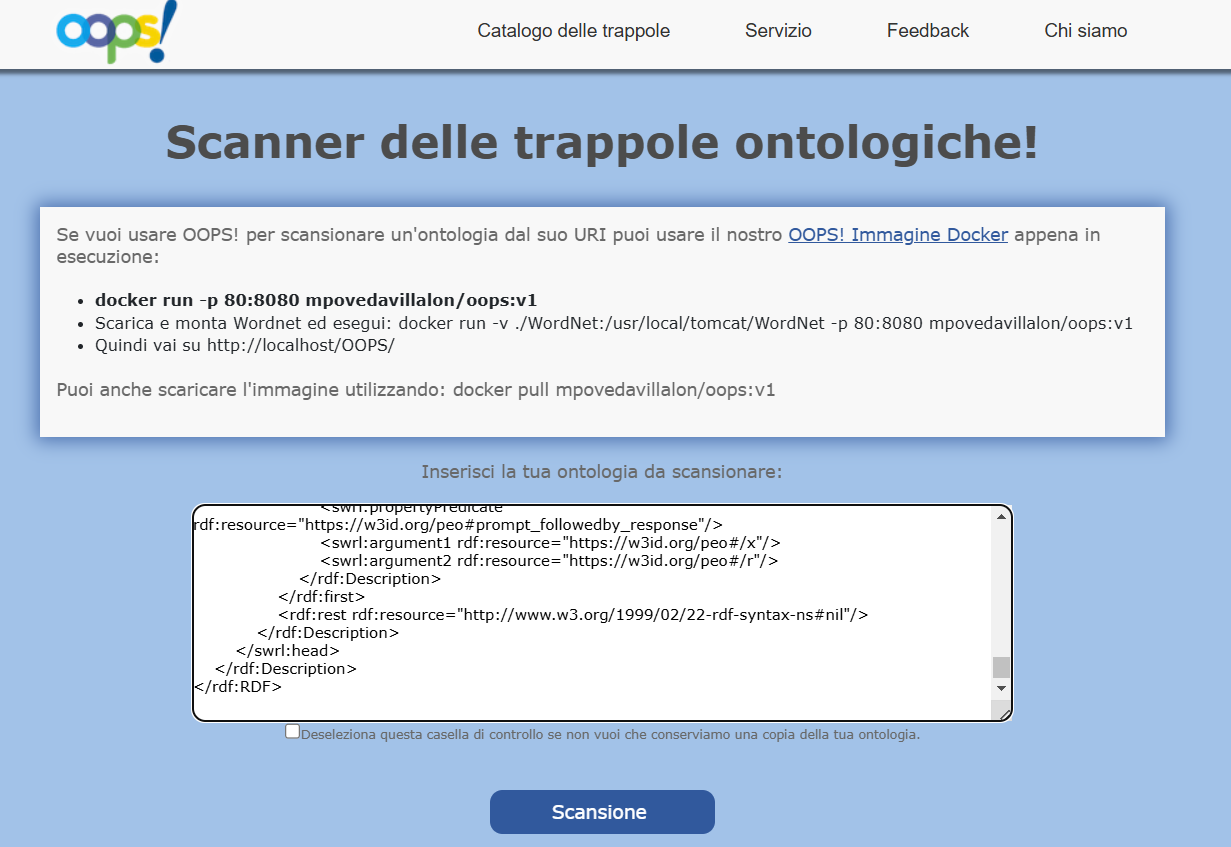
\includegraphics[width=0.9\linewidth]{Figures/fig_42.png}
    \caption{OOPS! web interface}
    \label{fig:42}
\end{figure}
Fig \ref{fig:42} shows the oops web interface.
Given the input ontology, OOPS is able to detect 40 different pitfall that are classified into three categories: critical, important and minor by parsing the RDF code and generating a complete response using the OOPS! scanner. Pitfalls in the scanner include:
\begin{itemize}
    \item Structural pitfalls: formal structure and syntax like cycles in hierarchy and unconnected ontology elements.

    \item Functional pitfalls: use and functionality of the ontology like missing domain or incorrectly defined inverse relationships.

    \item Usability and Profiling Pitfalls: clarity, maintainability, and human-readability like missing annotations, inconsistent naming and ambiguous terms.
\end{itemize}
I will use OOPS! scanner on both versions of the PEO detecting and explaining found pitfalls. 
For the first version of PEO there are just three pitfalls:
\begin{figure}[H]
    \centering
    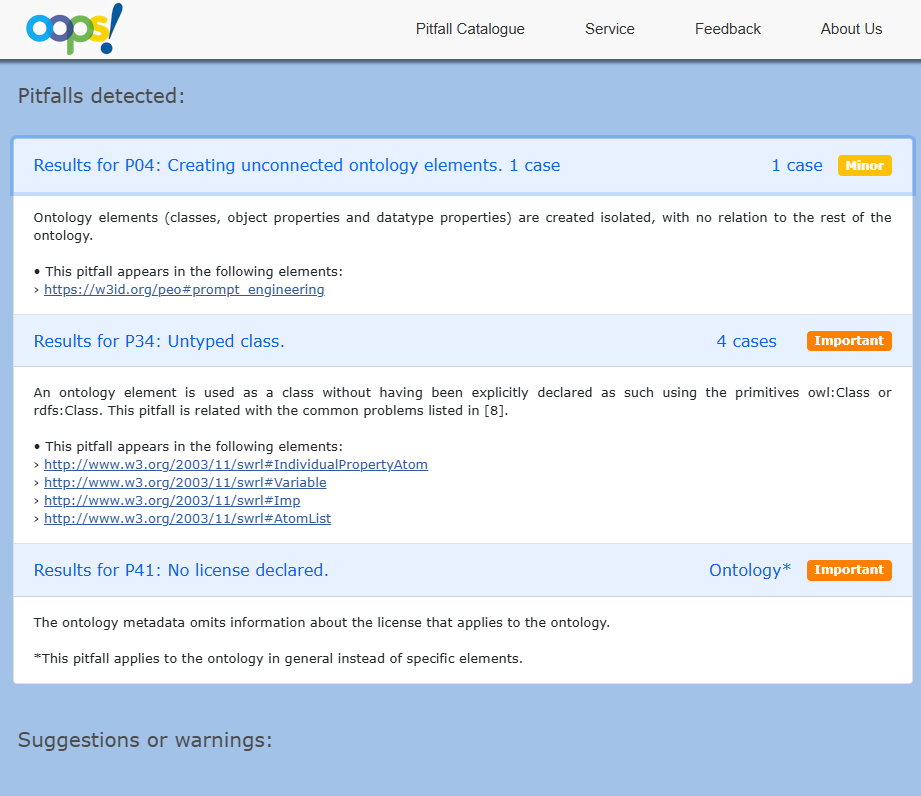
\includegraphics[width=0.9\linewidth]{Figures/fig_43.png}
    \caption{Detected pitfalls PEO}
    \label{fig:enter-label}
\end{figure}
The explanation of detected pitfall is:
\begin{itemize}
    \item P04 (Creating unconnected ontology elements): this pitfall involves ontology elements (classes, object properties and datatype properties) are created isolated, with no relation to the rest of the ontology. 

    \item P34 (Untyped class): this pitfalls involves all ontology elements that are used as a class without having explicitly declared. This pitfall involves four elements in PEO: \\ http://www.w3.org/2003/11/swrl\#IndividualPropertyAtom,\\ http://www.w3.org/2003/11/swrl\#Variable,\\ http://www.w3.org/2003/11/swrl\#Imp and \\http://www.w3.org/2003/11/swrl\#AtomList.

    \item P41 (No license declared): there is no license in the ontology metadata.    
\end{itemize}
Overall, the report is satisfactory, as no critical pitfalls have been identified, nor any issues found in the main classes or object properties of the ontology and I will discuss in more detail in Results discussion section.
The complete report is available here \footnote{https://github.com/simonegramegna/peo/blob/main/evaluation/oops\_report\_peo.xml}. After detecting pitfalls in the original version of the PEO, I also examined the populated version generated using GPT-4 nonetheless, no significant differences were observed between the two versions. Compared to the three pitfalls identified in the previous version, OOPS detects five pitfalls:
\begin{figure}[H]
    \centering
    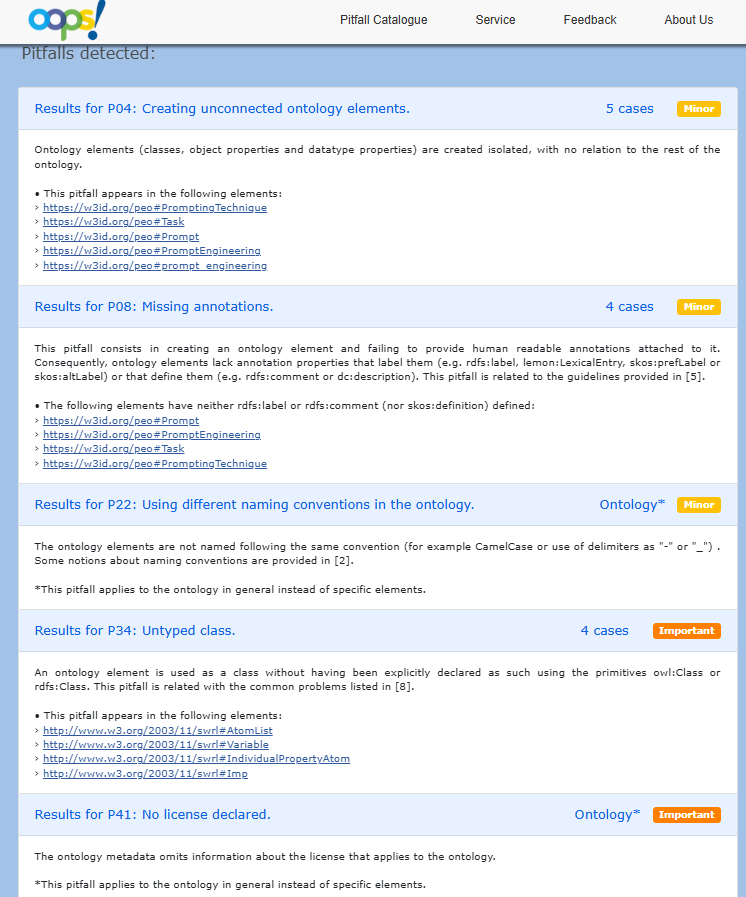
\includegraphics[width=0.75\linewidth]{Figures/fig_44.png}
    \caption{Detected pitfalls second version PEO}
    \label{fig:enter-label}
\end{figure}


\begin{itemize}
    \item P04 (Creating unconnected ontology elements): this pitfall, as said before, involves unconnected ontology elements. This time the pitfall involves not only the prompt\_engineering class but also the new classes created by GPT-4: Task, PromptingTechnique, Prompt and PromptEngineering. Those classes have no relations with other classes.

    \item P08 (Missing annotations): this pitfall involves elements that lack annotation properties that label them ( rdfs:label) or that define them\\ (rdfs:comment). This pitall involves the four classes created by GPT-4 with no comment provided: Task, PromptingTechnique, Prompt and PromptEngineering.  

    \item P22 (Using different naming conventions in the ontology): this pitfall involves ontology elements are not named following the same convention (for example CamelCase or use of delimiters as "-" or "\_"). This pitfall is given by the new classes created by GPT-4 that do not follow the naming convention used in the ontology (with the "\_" separator) by creating classes declared in camel case.

    \item P34 (Untyped class): this is the same pitfall detected before.

    \item P41 (No license declared): this is the same pitfall detected before.
\end{itemize}
In general, the detected pitfalls are caused by GPT-4's lack of understanding of the ontology's structure and I will discuss in more detail in the Results discussion section. The oops report is available here \footnote{https://github.com/simonegramegna/peo/blob/main/evaluation/oops_report_peo_gpt4.xml}.


\section{Competency Questions}
\label{section:5_4_cqs}
The final step of ontology evaluation is converting the CQs defined in the Ontology requirements specification section into SPARQL queries in order to compare the expected result to the actual result of each CQ.
SPARQL queries are generated manually and executed using Jupyter notebook \footnote{https://jupyter.org/}: an enviroment for running python code and the rdflib python library rdflib \footnote{https://rdflib.readthedocs.io/en/stable/}: a library to access rdf files and run SPARQL queries inside python.
The code is available in the  Github repository  \footnote{https://github.com/simonegramegna/peo/tree/main/evaluation}.
The evaluation is mode for both versions of the ontology.\\
Firstly, the ontology is loaded with rdflib as represented in fig. \ref{fig:45}
\begin{figure}[H]
    \centering
    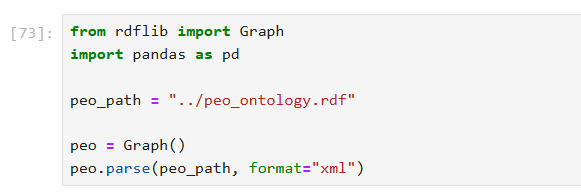
\includegraphics[width=0.9\linewidth]{Figures/fig_45.png}
    \caption{Jupyter notebook SPARQL}
    \label{fig:45}
\end{figure}
The pandas library is used to display query results in data-frames.
For such purpose, we implemented three helper functions:
\begin{itemize}
    \item execute\_query: it takes as input the SPARQL query string and returns a list of results.

    \item results\_to\_df: it takes as input as input the list of results ad creates and returns a dataframe with results inside which columns' names are the label names.

    \item print\_results: it iterates on the list of results and prints each element.
\end{itemize}
We can see the implementation below, in fig. \ref{fig:46}:
\begin{figure}[H]
    \centering
    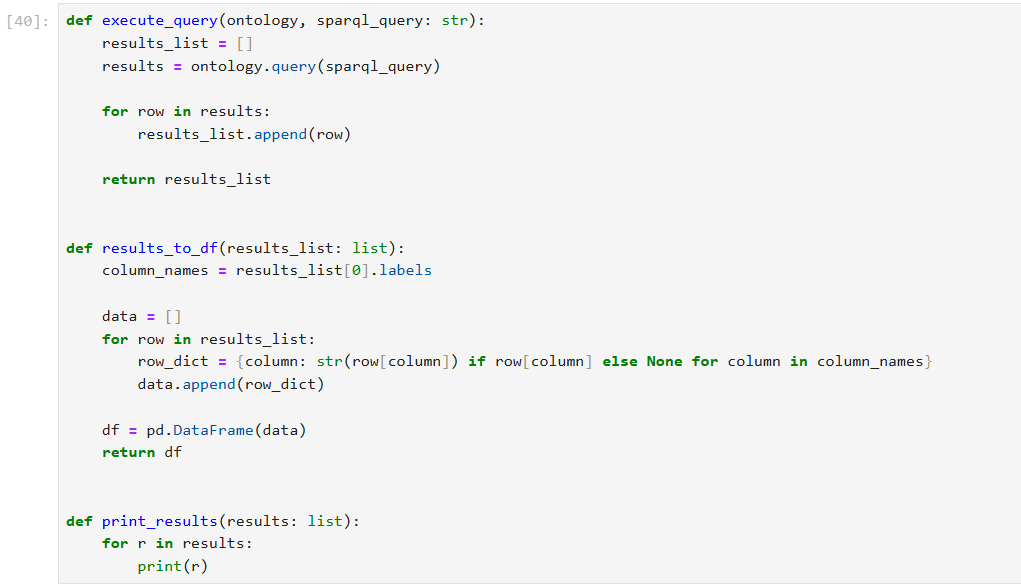
\includegraphics[width=0.9\linewidth]{Figures/fig_46.png}
    \caption{Support python functions}
    \label{fig:46}
\end{figure}

Once this is done, we can translate each of the sixteen CQs into SPARQL queries to be executed on PEO.\\
The first CQ CQ1: What is prompt engineering? is translated into:
\begin{lstlisting}
    SELECT DISTINCT ?property ?value
    WHERE {
        <https://w3id.org/peo#prompt_engineering> ?property ?value .
    }
\end{lstlisting}
\begin{figure}[H]
    \centering
    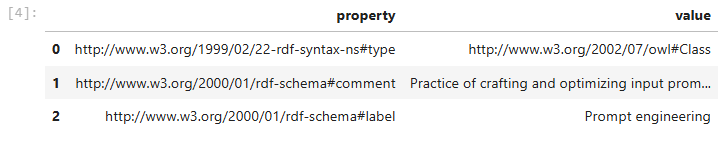
\includegraphics[width=0.9\linewidth]{Figures/fig_47.png}
    \caption{CQ1 SPARQL query results}
    \label{fig:47}
\end{figure}
The output, in fig. \ref{fig:47}, from the query matches the expected result, which is the definition of prompt engineering.\\

The second competency question CQ2: What is a prompt? is translated into:
\begin{lstlisting}
SELECT DISTINCT ?property ?value
WHERE {
    <https://w3id.org/peo#prompt> ?property ?value .
}
\end{lstlisting}
\begin{figure}[H]
    \centering
    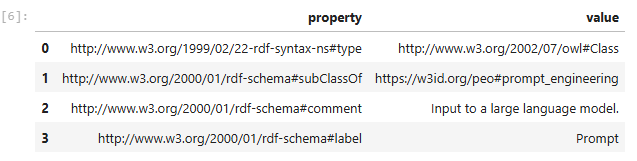
\includegraphics[width=0.9\linewidth]{Figures/fig_48.png}
    \caption{CQ2 SPARQL query results}
    \label{fig:48}
\end{figure}

The output, in fig. \ref{fig:48}, also in this case matches the expected result, which is the definition of prompt.\\

The third competency question CQ3: What are prompting techniques? is translated into:
\begin{lstlisting}
SELECT DISTINCT ?subclass ?label
WHERE {
    ?subclass rdfs:subClassOf <https://w3id.org/peo#prompting_technique> .
    OPTIONAL { ?subclass rdfs:label ?label . }
}
\end{lstlisting}

\begin{figure}[H]
    \centering
    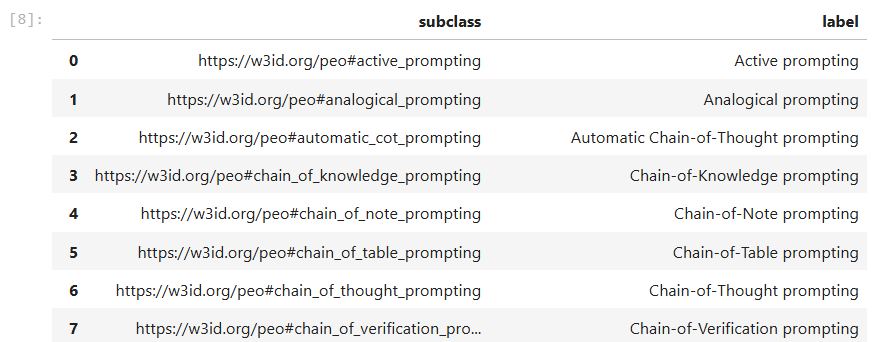
\includegraphics[width=0.9\linewidth]{Figures/fig_49.png}
    \caption{CQ3 SPARQL query results}
    \label{fig:49}
\end{figure}
The complete table contains, in fig. \ref{fig:49}, all the prompting techniques in the ontology.\\

The fourth competency question CQ4: What are image prompting techniques? is translated into:
\begin{lstlisting}
SELECT DISTINCT ?subclass ?label
WHERE {
    ?subclass rdfs:subClassOf <https://w3id.org/peo#image_prompting> .
    OPTIONAL { ?subclass rdfs:label ?label . }
}
\end{lstlisting}

\begin{figure}[H]
    \centering
    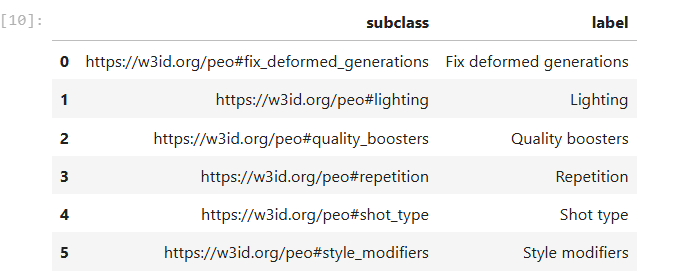
\includegraphics[width=0.9\linewidth]{Figures/fig_50.png}
    \caption{CQ4 SPARQL query results}
    \label{fig:50}
\end{figure}
As expected. in fig \ref{fig:50}, we get all the image prompting techniques in the ontology.\\

The fifth competency question CQ5: What are code prompting techniques? is translated into:
\begin{lstlisting}
SELECT DISTINCT ?subclass ?label
WHERE {
    ?subclass rdfs:subClassOf <https://w3id.org/peo#code_prompting> .
    OPTIONAL { ?subclass rdfs:label ?label . }
}  
\end{lstlisting}

\begin{figure}[H]
    \centering
    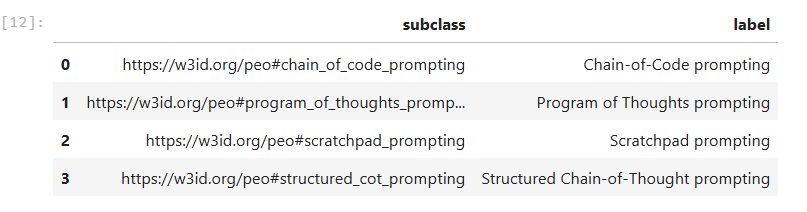
\includegraphics[width=0.9\linewidth]{Figures/fig_51.png}
    \caption{CQ5 SPARQL query results}
    \label{fig:51}
\end{figure}
The table contains, in \ref{fig:51}, all the code prompting techniques in the ontology.\\

The sixth competency question CQ6: Which task does a prompt solve? is translated into:
\begin{lstlisting}
SELECT DISTINCT ?prompt ?task ?taskLabel
WHERE {
    ?prompt <https://w3id.org/peo#solves> ?task .
    OPTIONAL { ?task rdfs:label ?taskLabel . }
}
\end{lstlisting}

\begin{figure}[H]
    \centering
    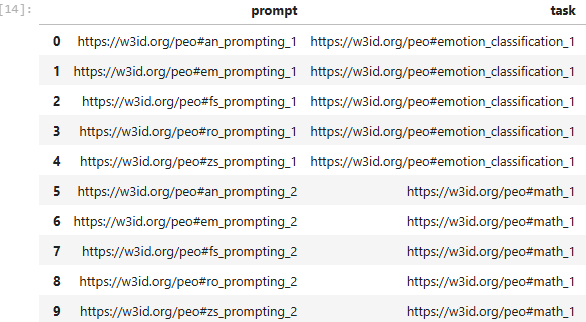
\includegraphics[width=0.9\linewidth]{Figures/fig_52.png}
    \caption{CQ6 SPARQL query results}
    \label{fig:52}
\end{figure}
The table contains, in fig \ref{fig:52}, all the prompts that solve tasks.\\

The seventh competency question CQ7: Which prompts are generated using a prompting technique? is translated into:
\begin{lstlisting}
SELECT DISTINCT ?prompt ?technique ?techniqueLabel
WHERE {
    ?prompt <https://w3id.org/peo#prompt_generated_using> ?technique .
    OPTIONAL { ?technique rdfs:label ?techniqueLabel . }
}
\end{lstlisting}

\begin{figure}[H]
    \centering
    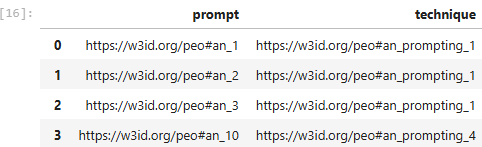
\includegraphics[width=0.9\linewidth]{Figures/fig_53.png}
    \caption{CQ7 SPARQL query results}
    \label{fig:53}
\end{figure}
The complete table, in fig \ref{fig:53}, contains all the prompt instances generated using instances of prompting techniques.\\

The eighth competency question CQ8: What are the responses that follow each prompt? is translated into:
\begin{lstlisting}
SELECT DISTINCT ?prompt ?response
WHERE {
    ?response <https://w3id.org/peo#response_followedby_prompt> ?prompt .
}    
\end{lstlisting}

\begin{figure}[H]
    \centering
    \includegraphics[width=0.9\linewidth]{Figures/fig_54.png}
    \caption{CQ8 SPARQL query results}
    \label{fig:54}
\end{figure}
The complete table contains, in fig. \ref{fig:54}, all the responses of all prompt instances.\\

The ninth competency question CQ9: What are possible tasks? is translated into:
\begin{lstlisting}
SELECT DISTINCT ?task ?label
WHERE {
    ?task rdf:type owl:Class .
    ?task rdfs:subClassOf* <https://w3id.org/peo#task> .
    OPTIONAL { ?task rdfs:label ?label . }
}    
\end{lstlisting}

\begin{figure}[H]
    \centering
    \includegraphics[width=0.9\linewidth]{Figures/fig_55.png}
    \caption{CQ9 SPARQL query results}
    \label{fig:55}
\end{figure}
In the completed table, in \ref{fig:55}, we get all the possible task represented in the ontology.\\

The tenth competency question CQ10: Which tasks are related to the text? is translated into:
\begin{lstlisting}
SELECT DISTINCT ?task ?label
WHERE {
    ?task rdf:type owl:Class .
    ?task rdfs:subClassOf* <https://w3id.org/peo#text_task> .
    OPTIONAL { ?task rdfs:label ?label . }
}
\end{lstlisting}

\begin{figure}[H]
    \centering
    \includegraphics[width=0.9\linewidth]{Figures/fig_56.png}
    \caption{CQ10 SPARQL query results}
    \label{fig:56}
\end{figure}

The resulting table, in fig. \ref{fig:56}, contains, all the task related to text.\\

The eleventh competency question CQ11: What is a chat? is translated into:
\begin{lstlisting}
SELECT DISTINCT ?property ?value
WHERE {
    <https://w3id.org/peo#chat> ?property ?value .
}
\end{lstlisting}

\begin{figure}[H]
    \centering
    \includegraphics[width=0.9\linewidth]{Figures/fig_57.png}
    \caption{CQ11 SPARQL query results}
    \label{fig:57}
\end{figure}
The result, in fig. \ref{fig:57}, is the definition of Chat.\\

The twelfth competency question CQ12: What is a large language model? is translated into:
\begin{lstlisting}
SELECT DISTINCT ?property ?value
WHERE {
    <https://w3id.org/peo#large_language_model> ?property ?value .
}
\end{lstlisting}

\begin{figure}[H]
    \centering
    \includegraphics[width=0.9\linewidth]{Figures/fig_58.png}
    \caption{CQ12 SPARQL query results}
    \label{fig:58}
\end{figure}
The result, in fig \ref{fig:58}, is the definition of Large Language Model.\\

The thirteenth competency question CQ13: What types of large language models are available? is translated into:
\begin{lstlisting}
SELECT DISTINCT ?type ?label
WHERE {
    ?type rdfs:subClassOf <https://w3id.org/peo#large_language_model> .
    OPTIONAL { ?type rdfs:label ?label . }
}
\end{lstlisting}

\begin{figure}[H]
    \centering
    \includegraphics[width=0.9\linewidth]{Figures/fig_59.png}
    \caption{CQ13 SPARQL query results}
    \label{fig:59}
\end{figure}
The resulting complete table, in fig. \ref{fig:59}, is the collection of all large language models represented in the ontology.\\

The fourteenth competency question CQ14: What are large language models architectures? is translated into:
\begin{lstlisting}
SELECT DISTINCT ?type ?label
WHERE {
    ?type rdfs:subClassOf <https://w3id.org/peo#base_model> .
    OPTIONAL { ?type rdfs:label ?label . }
}   
\end{lstlisting}

\begin{figure}[H]
    \centering
    \includegraphics[width=0.9\linewidth]{Figures/fig_60.png}
    \caption{CQ14 SPARQL query results}
    \label{fig:60}
\end{figure}
The result, in fig. \ref{fig:60}, is the collection of main large language models architectures.\\

The fifteenth competency question CQ15: What are large language models capabilities? is translated into:
\begin{lstlisting}
SELECT DISTINCT ?type ?label
WHERE {
    ?type rdfs:subClassOf <https://w3id.org/peo#capability> .
    OPTIONAL { ?type rdfs:label ?label . }
}
\end{lstlisting}

\begin{figure}[H]
    \centering
    \includegraphics[width=0.8\linewidth]{Figures/fig_61.png}
    \caption{CQ15 SPARQL query results}
    \label{fig:61}
\end{figure}
Results are represented, in fig. \ref{fig:61}, by the collection of all the capabilities represented in PEO.\\

The sixteenth and last competency question CQ16: What companies develop large language models? is translated into:
\begin{lstlisting}
SELECT DISTINCT ?company ?label
WHERE {
    ?company rdf:type <https://w3id.org/peo#company> .
    OPTIONAL { ?company rdfs:label ?label . }
}
\end{lstlisting}

\begin{figure}[H]
    \centering
    \includegraphics[width=0.8\linewidth]{Figures/fig_62.png}
    \caption{CQ16 SPARQL query results}
    \label{fig:62}
\end{figure}
The result, in fig. \ref{62}, is the collection of companies that develop large language models.\\
We proceed also, to execute SPARQL queries on the second version of PEO, the one that has been populated automatically using GPT-4. 
We translated only competency questions that match changes introduced by the LLM. Competency questions chosen for translation are four: CQ1, CQ2, CQ3 and CQ9.\\
The first competency question CQ1: What is prompt engineering? is translated into:
\begin{lstlisting}
SELECT DISTINCT ?property ?value
WHERE {
    <https://w3id.org/peo#PromptEngineering> ?property ?value .
} 
\end{lstlisting}

\begin{figure}[H]
    \centering
    \includegraphics[width=0.9\linewidth]{Figures/fig_69.png}
    \caption{CQ1 SPARQL query results - PEO updated}
    \label{fig:69}
\end{figure}
Fig. \ref{fig:69} shows the new output of CQ1.

The second competency question CQ2: What is a prompt? is translated
into:
\begin{lstlisting}
SELECT DISTINCT ?property ?value
WHERE {
    <https://w3id.org/peo#Prompt> ?property ?value .
}
\end{lstlisting}

\begin{figure}[H]
    \centering
    \includegraphics[width=0.9\linewidth]{Figures/fig_70.png}
    \caption{CQ2 SPARQL query results - PEO updated}
    \label{fig:70}
\end{figure}
Fig. \ref{fig:70} shows the new output of CQ2.

The third competency question CQ3: What are prompting techniques?
is translated into:
\begin{lstlisting}
SELECT DISTINCT ?instance
WHERE {
  ?instance <http://www.w3.org/1999/02/22-rdf-syntax-ns#type> <https://w3id.org/peo#PromptingTechnique> .
}
\end{lstlisting}


\begin{figure}[H]
    \centering
    \includegraphics[width=0.7\linewidth]{Figures/fig_71.png}
    \caption{CQ3 SPARQL query results - PEO updated}
    \label{fig:71}
\end{figure}
Fig. \ref{fig:71} shows the new output of CQ3.

The ninth competency question CQ9: What are possible tasks? is translated into:
\begin{lstlisting}
SELECT DISTINCT ?instance
WHERE {
  ?instance <http://www.w3.org/1999/02/22-rdf-syntax-ns#type> <https://w3id.org/peo#Task> .
}
\end{lstlisting}

\begin{figure}[H]
    \centering
    \includegraphics[width=0.6\linewidth]{Figures/fig_72.png}
    \caption{CQ9 SPARQL query results - PEO updated}
    \label{fig:72}
\end{figure}

Fig. \ref{fig:72} shows the new output of CQ9.


\section{Publication}
\label{section:5_5_publication}
The last step after the Ontology implementation in the LOT methodology is the Ontology publication phase, which scope is to provide an online ontology accessible both as human-readable documentation and a machine-readable documentation from its URI.
This phase is divided into three sub-activities:
\begin{enumerate}
    \item Propose release candidate
    \item Ontology documentation
    \item Online publication
\end{enumerate}
as we can see in the figure below:
\begin{figure}[H]
    \centering
    \includegraphics[width=0.9\linewidth]{Figures/fig_25.png}
    \caption{Ontology publication workflow}
    \label{fig:enter-label}
\end{figure}

\subsection{Propose Release Candidate}
\label{subsection:4_5_1_release}
After all the implementation and evaluation, in this step there is the decision about which version of the ontology is going to be published.
It is a quite easy choice because, as said in pervious sections, the version populated automatically did not add any useful information from the original version.
Moreover it added, according the OOPS! report, more pitfalls (five vs three).
\subsection{Ontology Documentation}
\label{subsection:4_5_2_docs}
The ontology documentation is generated using Protegé and the OWLdoc plug-in, which automatically generate HTML documentation starting from ontology code.
The output of OWLdoc is the following:
\begin{figure}[H]
    \centering
    \includegraphics[width=0.9\linewidth]{Figures/fig_63.png}
    \caption{OWLdoc output}
    \label{fig:enter-label}
\end{figure}
The OWLdoc is available in the GitHub repository here \footnote{https://github.com/simonegramegna/peo/tree/main/docs} in the /docs folder and it can be consulted online here \footnote{https://peoontology.vercel.app/}
The documentation is made accessible for everyone using Vercel: a cloud platform for hosting web applications and static sites.
This free service using an integrated Github action, takes as input the documentation in the repository and publishes online automatically without requiring any effort by the developer.
The official documentation website is:
\href{https://peoontology.vercel.app/}{https://peoontology.vercel.app/}.

\subsection{Online Publication}
\label{subsection:4_5_3_publication}
Once the ontology documentation is ready, the ontology can be published online on major vocabularies repository, by accessing the ontology using its URI. I will consider two most known repositories for ontology publishing: \href{https://w3id.org/}{w3id.org} and \href{https://bioportal.bioontology.org/}{BioPortal}.

W3id.org a permanent identifier service that provides stable, persistent, and HTTP-resolvable URIs for web resource. The creation of a new identifier for publishing a new ontology is made using Github and the official W3id.org Github repository. The procedure followed is straightforward, first we fork the W3id.org Github repository on my Github, creating a "copy" of the repository. 
\begin{figure}[H]
    \centering
    \includegraphics[width=0.9\linewidth]{Figures/fig_65.png}
    \caption{Forked W3id.org repository}
    \label{fig:enter-label}
\end{figure}
Then we create a new branch and we create a new directory with the intended permanent identifier name, in my case we create a directory called "peo". Inside this directory we create two files:
\begin{itemize}
    \item README.md: contains more identifier info and contact info, for human to read.
    \item .htaccess: contains redirection rules, for computer to read and perform.
\end{itemize}
In the case of PEO, the README.md contains all my contact information with the link to the PEO Github repository while the .htaccess contains the following redirections rules:
\begin{lstlisting}
# Activates Rewrite Engine
RewriteEngine On

# Content negotiation for RDF/XML
RewriteCond %{HTTP_ACCEPT} application/rdf\+xml
RewriteRule ^$ https://raw.githubusercontent.com/simonegramegna/peo/refs/heads/main/peo_ontology.rdf [R=303,L]

# Content negotiation for Turtle
RewriteCond %{HTTP_ACCEPT} text/turtle
RewriteRule ^$ https://raw.githubusercontent.com/simonegramegna/peo/refs/heads/main/peo_ontology.ttl [R=303,L]

# Default: serves HTML for browser or client not RDF-aware
RewriteRule ^$ https://peoontology.vercel.app/ [R=303,L]

# Blocks directory indexing
Options -Indexes
\end{lstlisting}
Once the two files are completed, we submitted a pull request to the main branch that is approved by one of repository administrators. As soon the merge of the created branch, it is possible to access to the ontology using its URI, in the case of PEO the URI is: \href{https://w3id.org/peo}{https://w3id.org/peo} bringing the user with an HTTP request to the online ontology documentation.
\begin{figure}[H]
    \centering
    \includegraphics[width=0.9\linewidth]{Figures/fig_66.png}
    \caption{W3id.org repository main directory}
    \label{fig:66}
\end{figure}
Fig. \ref{fig:66} shows W3id.org repository main directory

We decided to publish PEO also on BioPortal\footnote{https://bioportal.bioontology.org/
}. First we create an account on BioPortal and then we specify all the informations about the ontology: the version, the type (RDF) and the release date.
\begin{figure}[H]
    \centering
    \includegraphics[width=0.9\linewidth]{Figures/fig_67.png}
    \caption{BioPortal main page}
    \label{fig:enter-label}
\end{figure}
The ontology is published here \footnote{https://bioportal.bioontology.org/ontologies/PEO_ONTOLOGY?p=summary} and it is possible using the web interface view the whole ontology: classes, object properties, data properties and individuals. This is a very useful feature because the user has no need to download any additional software, moreover BioPortal computes automatically base ontology metrics. 
\begin{figure}[H]
    \centering
    \includegraphics[width=0.9\linewidth]{Figures/fig_68.png}
    \caption{BioPortal ontology interface}
    \label{fig:enter-label}
\end{figure}


\newpage
\section{Results Discussion}
\label{section:5_6_discussion}
The design and implementation phases led the creation of an ontology that is the very first to comprehensively and exhaustively represent prompt engineering techniques and large language models.
As discussed in previous chapters, resources on these topics are often quite limited and fragmented.
So PEO becomes an important reference in these fields providing users with a useful and effective. PEO also supports developers and researchers in choosing the best prompt engineering techniques and LLM for their scopes. Additionally, it assists content creators and copywriters in selecting the most suitable approach and model for automatic content creation.

The results obtained during the evaluation process of PEO reveal important insights into its design, structure, and functionality.
Through a combination of tools and methods, such as HermiT reasoner, OntoMetrics, and OOPS! validation, the ontology was rigorously assessed, highlighting both its strengths and areas for improvement.

There are three main strengths of the PEO found during the evaluation:
\begin{enumerate}
    \item Logical Consistency and Reasoning: the HermiT reasoner confirmed that the ontology's logical structure is sound, with no inconsistencies detected in both the manually populated version and the updated version generated by GPT-4. Moreover, additional triples and axioms are inferred. 

    \item Expressiveness and Structural Metrics: OntoMetrics demonstrated the ontology’s comprehensiveness, with 2684 axioms and $SRIF(D)$ expressivity, supporting advanced reasoning while maintaining computational efficiency. The hierarchical organization (199 SubClassOf axioms) facilitates inheritance.
    Moreover, the inclusion of 352 individuals indicates practical applicability.

    \item Semantic Coverage: competency questions translated into SPARQL queries yielded the expected results, confirming that the ontology effectively represents key concepts, such as prompting techniques, tasks, and the relationships between prompts and their generated responses. This shows that the ontology is well-aligned with its design goals.
\end{enumerate}

The evaluation found also the following limitations:
\begin{itemize}
    \item Pitfalls in Structure: OOPS! detected structural
    issues, such as unconnected elements and missing annotations. These issues were more 
    in the GPT-4-populated version, where newly introduced classes (e.g., Task, PromptingTechnique) lacked connections to the broader ontology. This indicates that automated population requires further refinement.

    \item Simplistic Relationships: metrics such as low relationship richness (0.160338) suggest that the ontology is more focused on defining concepts than on establishing interconnections. While this simplifies reasoning, it may limit the representation of complex semantic relationships.

    \item Underutilized Properties: object and data property axioms reveal limited use of features such as functional, symmetric, or inverse properties. Incorporating these could enhance the ontology's ability to model constraints and unique relationships.

    \item Inconsistencies in Naming Conventions: the naming conventions of new classes in the other version of PEO introduced by GPT-4 deviated from the original ontology’s standards, potentially affecting usability and integration.
\end{itemize}
In general, the major issues are present in the version of the PEO populated using GPT-4, as, as previously observed, it has not proven capable of correctly populating the original version of the ontology with new instances. Regarding the original version of the PEO, there are solvable pitfalls, which I will discuss in the next section.


Considering the limitations outlined in the previous section, caused by the pitfalls in the main version of the PEO, we proceed to address and correct the identified pitfalls:
\begin{itemize}
    \item P04 - Creating unconnected ontology elements: this pitfall involves the prompt\_engineering class which has no relation with any other class in the ontology.

    \item P34 - Untyped class: this pitfall involves elements in SWRL rules.

    \item P41 - No license declared: this pitfall is due to the absence of the license in the ontology.
\end{itemize}
The resolution of these pitfalls is essential to enhance the quality of the published ontology.

The pitfall P04, as said before, involves the prompt\_engineering class which has no relation with any other class in the ontology, this because the prompt\_engineering is a sort of "container" of classes related to prompt. In order to connect prompt\_engineering we created the object property applied\_to (with inverse relation supports) which connects prompt\_engineering with the large\_language\_model class.

\begin{figure}[H]
    \centering
    \includegraphics[width=0.7\linewidth]{Figures/fig_78.png}
    \caption{Object property between Prompt Engineering class and Large Language Model class}
    \label{fig:enter-label}
\end{figure}

The pitfall P34 stems from constructs automatically created by Protegé when a SWRL rule is defined.
In fact, SWRL is not part of the OWL languages so the types of the variables are not recognized.
To address this issue, we removed the SWRL rules and replaced them with property chains defined in OWL.
In this way, it is possible not only to reduce complexity, as SWRL rules involve a non-negligible computational cost, but also to make the ontology more portable, given that not all reasoners support SWRL rules.\\
In this case, we replaced the SWRL rule:
\begin{lstlisting}
peo:develops(?c, ?x) ^ peo:has_variant(?x, ?y) -> peo:develops(?c, ?y)
\end{lstlisting}
with the following object property chain:
\begin{figure}[H]
    \centering
    \includegraphics[width=0.7\linewidth]{Figures/fig_81.png}
    \caption{Object property chaining for develops}
    \label{fig:enter-label}
\end{figure}
The same approach is applied to the other object properties. A particular case is the SWRL rule S2: 
\begin{lstlisting}
peo:evolves(?x, ?y) -> peo:has_variant(?x, ?y)
\end{lstlisting}
In which, instead of using the property chain, we define it directly as an object property evolves as sub property of has\_variant as we can see in the figure below:
\begin{figure}[H]
    \centering
    \includegraphics[width=0.9\linewidth]{Figures/fig_82.png}
    \caption{evolves object property}
    \label{fig:enter-label}
\end{figure}
When the HermiT reasoner is activated, the inferences derived from the property chains are equivalent to those produced by the SWRL rules.

The pitfall P41, as said before, is due to the absence of the license in the ontology.
In order to solve this pitfall, I added the annotation property dcterms:license  as in \cite{yusof2019malaysian} with the link of the license (GNU General Public License v3) as value. Fig. \ref{fig:79} as we can see in the figure below:
\begin{figure}[H]
    \centering
    \includegraphics[width=0.9\linewidth]{Figures/fig_79.png}
    \caption{License annotation in PEO}
    \label{fig:79}
\end{figure}
To solve this pitfall, instead of using software license like GNU General Public License, I used the Creative Commons license available at this link: \href{https://creativecommons.org/licenses/by/4.0/}{https://creativecommons.org/licenses/by/4.0/}.

During the revision phase, it has been noted that class, object properties and data properties name do not follow the Semantic Web naming conventions that establishes Camel Case for class names, with the first letter in upper case while for object properties and data properties the Camel Case is used but the first letter is in lower case.
For example the object property evolved\_from with this modification, it becomes evolvedFrom and the large\_language\_model class becomes LargeLanguageModel.


We stated two RQs in Chapter:
\begin{enumerate}
      \item RQ~1: Does PEO provide comprehensive and consistent knowledge on LLMs and prompt engineering?

    \item RQ~2: Can we use PEO to infer additional knowledge?
\end{enumerate}

At the end of the experimental evaluation, it is possible to give an answer to the RQs.
The answer to RQ 1, is: yes.
Based on the results obtained during the testing and evaluation phase, we can say that PEO provides comprehensive and consistent knowledge on LLMs and prompt engineering. The execution of SPARQL queries confirms that PEO is able to provide correct informations on concepts like prompt, prompting technique, large language models and task. From the analysis of the results obtained with OntoMetrics, PEO has a good number of classes (126) and individuals (352), with individuals interconnected through 34 object properties. The tangledness equal to 0.26 and the relationships richness equal to 0.16 demonstrates that PEO is not complex and it has moderate relations between concepts.

Also the answer to RQ 2 is: yes.
The inference mechanism and property chaining defined in the PEO makes possible to get informations about all the characteristics of each large language model represented and the connections with prompts generated using prompt engineering techniques. Minor issues highlighted by pitfalls have been resolved once identified, ensuring the quality of the final result.


Despite these minor issues, the PEO is well-designed, comprehensive, well-documented, and has very few problems.
It significantly outperforms state-of-the-art ontologies related to large language models and prompt engineering.

\chapter{Conclusions and Future Works}
\label{chapter:6_conclusions_future_developments}
In this concluding chapter, I present some final thoughts and propose potential directions for future research concerning the development of PEO.


\section{Conclusions}
\label{section:6_1_conclusions}
Inspired by the curiosity to explore an emerging field like prompt engineering and driven by the need to create a comprehensive resource that could be useful to those who share the same interest, we created PEO. During the design and encoding phases, we applied more modern techniques of ontology engineering. This allowed us to make PEO an ontology capable of fully describing all concepts related to prompt engineering and LLMs, considering the interconnections between them. Special attention was given to the experimentation and evaluation phase to ensure the quality of the ontology as well as its consistency with the specifications. The publication of all artifacts online, according to the FAIR principles, makes PEO visible and editable by any user under the Creative Commons license. Users can further advance the project through various future developments. 

\section{Future Works}
\label{section:6_2_future}
The future developments of the PEO ontology are numerous and can proceed in different yet complementary directions. 
Among these, we consider as interesting the following future developments:
\begin{itemize}
    \item Automatic population using LLMs: experiment with other LLMs and applying more advanced techniques for ontology population.
   
    \item Integration with external ontologies: integrate with the ontologies on LLMs 

    \item Improvement of the inference part: further enhance the expressivity of the TBox to gain even more inference capabilities.


    \item PEO-based AI agent: the development of a PEO-based AI agent can dynamically select and refine prompts based on user intent, task type, and LLM capabilities, optimizing interactions with language models. 
    
 
    \item PEO ontology web application: the development of a web application using HTML, CSS, and JavaScript to interact with the PEO ontology is a potential future advancement that could enhance its accessibility and support its wider adoption. 
\end{itemize}
The future developments that will be carried out will surely enhance PEO, a unique project never experimented that was casually born during a Teams call with my advisor on a warm day in mid-May 2024.


\chapter*{}
\textit{La mattina mi alzo e penso a vincere, vado a letto la sera e penso a vincere e quando sono in monoposto, non posso che pensare a vincere.}\\\\Charles Leclerc

%-------------------------------------------------------------------------------

%----------------------------------------------------------------------------------------
%	BIBLIOGRAPHY
%----------------------------------------------------------------------------------------

\printbibliography[heading=bibintoc]

\chapter*{}

\textit{Sì nu artìst!}\\\\Ruvo di Puglia, 23 febbraio 2025
%----------------------------------------------------------------------------------------

\end{document}  
